% A LaTeX template for MSc Thesis submissions to
% Politecnico di Milano (PoliMi) - School of Industrial and Information Engineering
%
% S. Bonetti, A. Gruttadauria, G. Mescolini, A. Zingaro
% e-mail: template-tesi-ingind@polimi.it
%
% Last Revision: October 2021
%
% Copyright 2021 Politecnico di Milano, Italy. NC-BY

\documentclass{Configuration_Files/PoliMi3i_thesis}

% CONFIGURATIONS
\usepackage{parskip} % For paragraph layout
\usepackage{setspace} % For using single or double spacing
\usepackage{emptypage} % To insert empty pages
\usepackage{multicol} % To write in multiple columns (executive summary)
\setlength\columnsep{15pt} % Column separation in executive summary
\setlength\parindent{0pt} % Indentation
\raggedbottom
\usepackage{multirow}

% PACKAGES FOR TITLES
\usepackage{titlesec}
% \titlespacing{\section}{left spacing}{before spacing}{after spacing}
\titlespacing{\section}{0pt}{3.3ex}{2ex}
\titlespacing{\subsection}{0pt}{3.3ex}{1.65ex}
\titlespacing{\subsubsection}{0pt}{3.3ex}{1ex}
\usepackage{color}

% PACKAGES FOR LANGUAGE AND FONT
\usepackage[english]{babel} % The document is in English  
\usepackage[utf8]{inputenc} % UTF8 encoding
\usepackage[T1]{fontenc} % Font encoding
\usepackage[11pt]{moresize} % Big fonts

% PACKAGES FOR IMAGES
\usepackage{graphicx}
\usepackage{transparent} % Enables transparent images
\usepackage{eso-pic} % For the background picture on the title page
\usepackage{subfig} % Numbered and caption subfigures using \subfloat.
\usepackage{tikz} % A package for high-quality hand-made figures.
\usetikzlibrary{}
\graphicspath{{./images/}} % Directory of the images
\usepackage{amsthm} % Coloured "Theorem"
\usepackage{thmtools}
\usepackage{xcolor}
\usepackage{float}

% STANDARD MATH PACKAGES
\usepackage{amsmath}
\usepackage{amssymb}
\usepackage{amsfonts}
\usepackage{bm}
\usepackage[overload]{empheq} % For braced-style systems of equations.
\usepackage{fix-cm} % To override original LaTeX restrictions on sizes

% PACKAGES FOR TABLES
\usepackage{tabularx}
\usepackage{longtable} % Tables that can span several pages
\usepackage{colortbl}

% PACKAGES FOR ALGORITHMS (PSEUDO-CODE)
\usepackage{algorithm}
\usepackage{algorithmic}

% PACKAGES FOR REFERENCES & BIBLIOGRAPHY
\usepackage[
    colorlinks=true,
    linkcolor=black,
    anchorcolor=black,
    citecolor=black,
    filecolor=black,
    menucolor=black,
    runcolor=black,
    urlcolor=black
]{hyperref} % Adds clickable links at references
\usepackage{cleveref}
\usepackage[square, numbers, sort&compress]{natbib} % Square brackets, citing references with numbers, citations sorted by appearance in the text and compressed
\bibliographystyle{abbrvnat} % You may use a different style adapted to your field

% OTHER PACKAGES
\usepackage[normalem]{ulem}
\usepackage{verbatim}
\usepackage[super]{nth}
\usepackage{pdfpages} % To include a pdf file
\usepackage{afterpage}
\usepackage{lipsum} % DUMMY PACKAGE
\usepackage{fancyhdr}
\usepackage{wasysym} % For the headers
\usepackage{rotating}
\usepackage{listings}
\usepackage{hyperref}
\usepackage{enumitem}
\fancyhf{}

% Input of configuration file. Do not change config.tex file unless you really know what you are doing. 
% Define blue color typical of polimi
\definecolor{bluepoli}{cmyk}{0.4,0.1,0,0.4}

% Custom theorem environments
\declaretheoremstyle[
    headfont=\color{bluepoli}\normalfont\bfseries,
    bodyfont=\color{black}\normalfont\itshape,
]{colored}

% Set-up caption colors
\captionsetup[figure]{labelfont={color=bluepoli}} % Set colour of the captions
\captionsetup[table]{labelfont={color=bluepoli}} % Set colour of the captions
\captionsetup[algorithm]{labelfont={color=bluepoli}} % Set colour of the captions

\theoremstyle{colored}
\newtheorem{theorem}{Theorem}[chapter]
\newtheorem{proposition}{Proposition}[chapter]

% Enhances the features of the standard "table" and "tabular" environments.
\newcommand\T{\rule{0pt}{2.6ex}}
\newcommand\B{\rule[-1.2ex]{0pt}{0pt}}

% Pseudo-code algorithm descriptions.
\newcounter{algsubstate}
\renewcommand{\thealgsubstate}{\alph{algsubstate}}
\newenvironment{algsubstates}
{\setcounter{algsubstate}{0}%
\renewcommand{\STATE}{%
    \stepcounter{algsubstate}%
    \Statex {\small\thealgsubstate:}\space}}
{}

% New font size
\newcommand\numfontsize{\@setfontsize\Huge{200}{60}}

% Title format: chapter
\titleformat{\chapter}[hang]{
    \fontsize{50}{20}\selectfont\bfseries\filright}{\textcolor{bluepoli} \thechapter\hsp\hspace{2mm}\textcolor{bluepoli}{|   }\hsp}{0pt}{\huge\bfseries \textcolor{bluepoli}
}

% Title format: section
\titleformat{\section}
{\color{bluepoli}\normalfont\Large\bfseries}
{\color{bluepoli}\thesection.}{1em}{}

% Title format: subsection
\titleformat{\subsection}
{\color{bluepoli}\normalfont\large\bfseries}
{\color{bluepoli}\thesubsection.}{1em}{}

% Title format: subsubsection
\titleformat{\subsubsection}
{\color{bluepoli}\normalfont\large\bfseries}
{\color{bluepoli}\thesubsubsection.}{1em}{}

% Shortening for setting no horizontal-spacing
\newcommand{\hsp}{\hspace{0pt}}

\makeatletter
% Renewcommand: cleardoublepage including the background pic
\renewcommand*\cleardoublepage{%
    \clearpage\if@twoside\ifodd\c@page\else
    \null
    \AddToShipoutPicture*{\BackgroundPic}
    \thispagestyle{empty}%
    \newpage
    \if@twocolumn\hbox{}\newpage\fi\fi\fi}
\makeatother

%For correctly numbering algorithms
\numberwithin{algorithm}{chapter}




\definecolor{dkgreen}{rgb}{0,0.6,0}
\definecolor{gray}{rgb}{0.5,0.5,0.5}
\definecolor{mauve}{rgb}{0.58,0,0.82}

%----------------------------------------------------------------------------
%	BEGIN OF YOUR DOCUMENT
%----------------------------------------------------------------------------

\begin{document}
    \fancypagestyle{plain}{%
        \fancyhf{} % Clear all header and footer fields
        \fancyhead[RO,RE]{\thepage} %RO=right odd, RE=right even
        \renewcommand{\headrulewidth}{0pt}
        \renewcommand{\footrulewidth}{0pt}}

%----------------------------------------------------------------------------
%	TITLE PAGE
%----------------------------------------------------------------------------

    \pagestyle{empty} % No page numbers
    \frontmatter % Use roman page numbering style (i, ii, iii, iv...) for the preamble pages

    \puttitle{
        title=Software Engineering 2\\Design Document,
        name1=Riccardo Piantoni - 10816545, % Author Name and Surname
        name2=Matteo Rossi - 10798975,
        name3=Jacopo Sacramone - 10752157,
        academicyear=2024-2025,
        version=1.0,
        releasedate=05/01/2025
          }
    
    
%----------------------------------------------------------------------------
%	PREAMBLE PAGES: ABSTRACT (inglese e italiano), EXECUTIVE SUMMARY
%----------------------------------------------------------------------------
    \startpreamble
    \setcounter{page}{1} % Set page counter to 1

%----------------------------------------------------------------------------
%	LIST OF CONTENTS/FIGURES/TABLES/SYMBOLS
%----------------------------------------------------------------------------

% TABLE OF CONTENTS
    \thispagestyle{empty}
    \tableofcontents % Table of contents
    \thispagestyle{empty}
    \cleardoublepage

%-------------------------------------------------------------------------
%	THESIS MAIN TEXT
%-------------------------------------------------------------------------

    \addtocontents{toc}{\vspace{2em}} % Add a gap in the Contents, for aesthetics
    \mainmatter % Begin numeric (1,2,3...) page numbering


    \chapter{Introduction}
    \label{ch:introduction}%
    \section{Purpose}
The transition from academia to the job market often presents significant challenges for university students, as they face difficulties in aligning their academic skills with industry expectations. Companies, on the other hand, struggle to efficiently connect with young talent and promote internships and job opportunities tailored to their needs. These gaps create inefficiencies in the hiring process, leaving valuable opportunities untapped.

\textbf{Students\&Companies} (S\&C) is designed to fill this gap. The platform aims to facilitate entrance into the job market for students while enabling companies to effectively reach and recruit emerging talent. By addressing the mismatch between academic preparation and industry requirements, S\&C enhances the matching process, creating an ecosystem where education meets practical experience.
\label{sec:purpose}%

\subsection{Goals}
\label{subsec:goals}%
\newcounter{g}
\setcounter{g}{1}
\newcommand{\cg}{\theg\stepcounter{g}}

\newcounter{subg}
\setcounter{subg}{1}
\newcommand{\csubg}{\thesubg\stepcounter{subg}}
\newcommand{\resetsubg}{\setcounter{subg}{1}}


In this section, there are defined the goals that the system has to achieve:

    \uline{\textbf{Profile Management}}

        \textbf{[G\cg]} Students, companies and universities should manage their profiles on the platform.

    \uline{\textbf{Internships Publication and Search}}
        
        \textbf{[G\cg]} Companies should advertise their internships.

        \textbf{[G\cg]} Students should apply for internships.

    \uline{\textbf{Recommendations}}
            
        \textbf{[G\cg]} Students should receive recommendations about internship offers matching their CVs.

        \textbf{[G\cg]} Companies should receive recommendations about students matching their preferences.

    \uline{\textbf{Selection Process}}

        \textbf{[G\cg]} Companies should manage the selection process aimed at evaluating candidates for their internship offers.
        
    \uline{\textbf{Monitoring}}

        \textbf{[G\cg]} Both students and companies should monitor the evolution of the internships they are taking part in. 

        \textbf{[G\cg]} Both students and companies should report complaints about the ongoing internships.

        \textbf{[G\cg]} Universities should handle complaints about the internships of their students.

        \textbf{[G\cg]} Both students and companies should provide feedback regarding the concluded internship they have taken part in.

    \uline{\textbf{Submission Suggestions}}

        \textbf{[G\cg]} Students should receive suggestions about how to make their CVs more appealing.
        
        \textbf{[G\cg]} Companies should receive suggestions about how to make their internship offers' descriptions more appealing.

\section{Scope}
\label{sec:scope}

\textbf{Students\&Companies} (S\&C) is a platform that acts as an intermediary system facilitating the internship matching process between students and companies. It allows companies to advertise internships and students to search, receive customized recommendations, and initiate contact.

The platform defines \textbf{Recommendation} as the automated process of identifying suitable internship opportunities for students and potential candidates for companies. Following this, a \textbf{Contact} represents the phase in which students and companies communicate via the platform to conduct the selection process, including interviews and candidate selection.

The system automates key activities such as generating recommendations using various mechanisms, coordinating interviews, and collecting feedback to improve its algorithms. Additionally, it provides tools to monitor the progress of contacts and internships, manage issues through communication features, and enable universities to supervise the status of internships, ensuring compliance and resolving possible complaints effectively.

\subsection{World Phenomena}
\label{subsec:world_phenomena}
\newcounter{wp}
\setcounter{wp}{1}
\newcommand{\cwp}{\thewp\stepcounter{wp}}

        \textbf{[WP\cwp]} Students redact their CV.

        \textbf{[WP\cwp]} Companies make new internship positions available.

        \textbf{[WP\cwp]} Students decide to take an internship.

        \textbf{[WP\cwp]} Companies select candidates to be interviewed among the applicants for each of their open positions.

        \textbf{[WP\cwp]} Companies select the student candidates who fit the most according to the results of their interviews.

        \textbf{[WP\cwp]} Students carry on their internships at their companies.

        \textbf{[WP\cwp]} A problem arises in an ongoing internship.
        
        \textbf{[WP\cwp]} Universities handle complaints (eventually interrupting internships).

\subsection{Shared Phenomena}
\label{subsec:shared_phenomena}
\newcounter{sp}
\setcounter{sp}{1}
\newcommand{\csp} {\thesp\stepcounter{sp}}

\uline{\textbf{World Controlled}}

        \textbf{[SP\csp]} Students, companies and universities sign up to the platform.

        \textbf{[SP\csp]} Students, companies and universities log into the platform.

        \textbf{[SP\csp]} Users provide information about themselves to the system.

        \textbf{[SP\csp]} Companies provide information about their internship positions to the system.

        \textbf{[SP\csp]} Students submit filters to search for suitable internship positions.

        \textbf{[SP\csp]} Students proactively apply for an open internship position.

        \textbf{[SP\csp]} Students track received recommendations about internship offers.

        \textbf{[SP\csp]} Companies track recommendations about potential candidates for their internship offers.

        \textbf{[SP\csp]} Students accept recommendations for internships.

        \textbf{[SP\csp]} Students reject recommendations for internships.
        
        \textbf{[SP\csp]} Companies accept recommended candidates for their internships. 

        \textbf{[SP\csp]} Companies reject recommended candidates for their internships. 
        
        \textbf{[SP\csp]} Companies contact selected students to set up an interview with them. 

        \textbf{[SP\csp]} Companies submit questions to students. 
        
        \textbf{[SP\csp]} Students provide the information required by companies during the interview.

        \textbf{[SP\csp]} Companies finalize the selection process.

        \textbf{[SP\csp]} Students track the outcomes of the interviews they have participated in.
        
        \textbf{[SP\csp]} Students and companies report information about an ongoing internship.

        \textbf{[SP\csp]} Students, companies and universities monitor an ongoing internship.
        
        \textbf{[SP\csp]} Students and companies report complaints and problems about ongoing internships.

        \textbf{[SP\csp]} Universities report information about the problems they have handled.

        \textbf{[SP\csp]} Students and companies provide feedback and suggestions about internships.

        \textbf{[SP\csp]} Students ask for suggestions about their profiles.

        \textbf{[SP\csp]} Companies ask for suggestions about their internship offers.

\uline{\textbf{Machine Controlled}}

        \textbf{[SP\csp]} The system shows to the students the internship offers which match their selection criteria.

        \textbf{[SP\csp]} The system shows to the companies the list of all the students who have applied for their internship offers.

        \textbf{[SP\csp]} The system shows to students and companies the list of all their received recommendations along with their status.

        \textbf{[SP\csp]} The system forwards communications about the scheduling of interviews from companies to students (and vice-versa).
        
        \textbf{[SP\csp]} The system forwards the submitted questions from companies to students.
        
        \textbf{[SP\csp]} The system forwards the submitted answers from students to companies, which collect them.

        \textbf{[SP\csp]} The system shows to the candidate students the outcome of their interviews after the conclusion of a selection process.

        \textbf{[SP\csp]} The system forwards information about the ongoing internships to students and companies.

        \textbf{[SP\csp]} The system forwards to universities information about problems in the ongoing internships of their students.

        \textbf{[SP\csp]} The system asks for feedback after the conclusion of an internship to improve its recommendation algorithms.        

        \textbf{[SP\csp]} The system provides suggestions to students about their profiles.

        \textbf{[SP\csp]} The system provides suggestions to companies about the description of their internship offers.

\section{Definitions, Acronyms, Abbreviations}
\label{sec:definition_acronyms_abbreviations}

\begin{itemize}

\item \textbf{System, Platform}: these terms are used interchangeably when referring to the system-to-be-developed.

\item \textbf{Upload a CV}: refers to completing all required fields in the CV section of the user's profile. This isn't an upload of a file to enforce a standardized format and enable the system to efficiently collect and process the information.

\item \textbf{University, Company}: when the terms are referenced as performing an action, it means that the action is executed by a representative acting on behalf of the respective entity.

\item \textbf{Party}: the term refers to the entities actively involved in the process of apply, participating and managing internships, so both Student and Company; it doesn't include the University.

\item \textbf{Platform Guidelines}: a set of rules and policies ensuring standardized behavior across users and maintaining the platform's integrity and usability.

\item \textbf{In-Platform vs. In-Person Interviews:}

\begin{itemize}
\item \textbf{In-Platform Interview}: Conducted entirely through the platform tools, such as structured questionnaires.
\item \textbf{In-Person Interviews}: Requires the candidate and interviewer to meet physically at a designated location.
\end{itemize}

\item \textbf{Accuracy}: represents the proportion of correct recommendations made by the system, calculated as the ratio of successful matches to the total number of recommendations generated. It provides an overall measure of how well the system performs.

\item \textbf{F1}: a performance metric that combines precision and recall into a single value, balancing the trade-off between the two. Precision measures the proportion of correct recommendations among all generated recommendations, while recall measures the proportion of relevant matches identified out of all possible relevant matches. The F1 score is particularly useful in evaluating the recommendation system when both false positives and false negatives are significant concerns.

\end{itemize}

\begin{table}[H]
    \begin{center}
        \begin{tabular}{ |l|l| }
            \hline
            \textbf{Acronyms} & \textbf{Definition}                              \\
            \hline
            RASD             & Requirements Analysis \& Specification Document   \\
            \hline
            API             & Application Programming Interface                  \\
            \hline
            HTTPS             & HyperText Transfer Protocol over Secure Socket Layer   \\
            \hline            
            2FA             &  Two-Factor Authentication \\
            \hline    
         \end{tabular}
        \caption{Acronyms used in the document.}
        \label{tab:acronyms}%
    \end{center}
\end{table}

\begin{table}[H]
    \begin{center}
        \begin{tabular}{ |l|l| }
            \hline
            \textbf{Abbreviations} & \textbf{Definition}
            \\
            \hline
            S\&C               & Student\&Company                     \\
            \hline
            G               & Goal                           \\
            \hline
            WP             & World Phenomena                          \\
            \hline
            SP             & Shared Phenomena                           \\
            \hline
            DA             & Domain Assumption                          \\
            \hline
            R              & Requirement                           \\
            \hline
            UC             & Use Case                           \\
            \hline
         \end{tabular}
        \caption{Abbreviations used in the document.}
        \label{tab:Abbreviations}%
    \end{center}
\end{table}

\section{Revision history}
\label{sec:revision_history}%
\label{sec:definition_acronyms_abbreviations}%
\begin{table}[H]
    \begin{center}
        \begin{tabular}{ |l|l|l|}
            \hline
            \textbf{Revised on} & \textbf{Version}   & \textbf{Description}                           \\
            \hline
            22/12/2024             & 1.0   &   Initial Release of the document  \\
            \hline
            05/01/2025             & 1.1   &   Update of the document according to Design Document decisions  \\
            \hline
         \end{tabular}
         \caption{Revision history}
        \label{tab:acronyms}%
    \end{center}
\end{table}

\paragraph{Integrations in Version 1.1}
\begin{itemize}
    \item Removed the misleading use of the concept of notification throughout the document to enhance clarity.
    \item Minor adjustments to Domain-level Class Diagram.
    \item Conformed User Interfaces section to UI design provided in Design Document.
    \item Updated UC1, UC2, UC3 by unifying the sign up process in the initial step of registration.
    \item Updated UC4 by adding an exception for missing profile information.
    \item Updated UC6. Publish an Internship Offer, changed the term \textit{Application domain} with \textit{Role}.
    \item Updated UC17. Handle Problems during an Internship to enhance clarity and better align the process with the interactions available through the university dashboard.
\end{itemize}

\newcounter{bib}
\setcounter{bib}{1}
\newcommand{\cbib} {\thebib\stepcounter{bib}}

\section{Reference Documents}
\label{sec:reference_documents}
\begin{itemize}
    \item{[\cbib]} Di Nitto, Rossi, Camilli, \textit{"A.Y. 2024-2025 Software Engineering 2 Requirement Engineering and Design Project"}, 2024.
    \item{[\cbib]} ISO/IEC/IEEE 29148:2018, \textit{"Systems and Software Engineering — Life Cycle Processes — Requirements Engineering," International Organization for Standardization, International Electrotechnical Commission, and Institute of Electrical and Electronics Engineers}, 2018.
\end{itemize}

\section{Document Structure}
\label{sec:document_structure}%
This document is composed of six sections:
\begin{itemize}
    \item{} \nth{1} Chapter - Introduction
    \item{} \nth{2} Chapter - Overall Description
    \item{} \nth{3} Chapter - Specific Requirements
    \item{} \nth{4} Chapter - Formal Analysis using Alloy
    \item{} \nth{5} Chapter - Effort Spent
    \item{} \nth{6} Chapter - References
\end{itemize}




    \chapter{Architectural Design}
    \label{ch:architectural_design}%
    \section{Overview: High-Level Components and Interactions}
\label{sec: overview}
In this section, a general description of the architecture of the S\&C system is provided.
The main architectural styles to be followed are:
\begin{itemize}
    \item \textbf{Client-Server Architecture:} This architecture was chosen for its simplicity and efficiency in managing user interactions and business logic. It is also scalable, as servers can be replicated and distributed to handle increasing user loads.
    \item \textbf{4-Tier Architecture:} The tier architecture and the number of levels are a natural consequence of the subdivision of functionalities across distinct layers, as it will be shown in the \hyperref[sec: deployment_view]{\uline{Deployment View}}. This approach supports a clear separation of concerns, ensuring each tier is responsible for a specific aspect of the system’s operation. This architecture enhances scalability, modularity and fault tolerance, separating each layer, and allows the system to adapt dynamically to workload demands while maintaining high availability and performance.
    \item \textbf{Microservices:} The system's functionalities have been split into separated microservices, each with its own dedicated database. This decision comes with plenty of benefits: for instance, it allows the achievement of better separation of concerns and decoupling between the functionalities offered, which consequently makes it possible to implement them in parallel and also to accomplish graceful degradation of the system in case of failures. Moreover, it enables different deployment strategies, such as containerization, enhancing system scalability.
    \item \textbf{REST - Representational State Transfer:} The designed microservices expose interfaces based on a REST API to communicate both with each other and the outside world. This decision allows to hide underlying technical aspects of the services since the communication is achieved through a technology-neutral protocol.
\end{itemize}

\newpage

\section{Component View}
\label{sec: component_view}

In this section, the main components of the S\&C system are outlined, with an accurate description of what each of them aims to accomplish. Every component is approximately derived from one of the product functions discussed in Section 2.2 of the RASD. Further, components are grouped together by affinity in high-level "macro-categories" to form microservices, obtaining what is usually referred to as "bounded contexts" in Domain-Driven Development (DDD). Components also expose interfaces with methods to be invoked from external entities and communicate with some databases.

\subsection{Component Diagram}
\label{subsec:component_diagram}
\begin{figure} [H]
    \begin{center}
        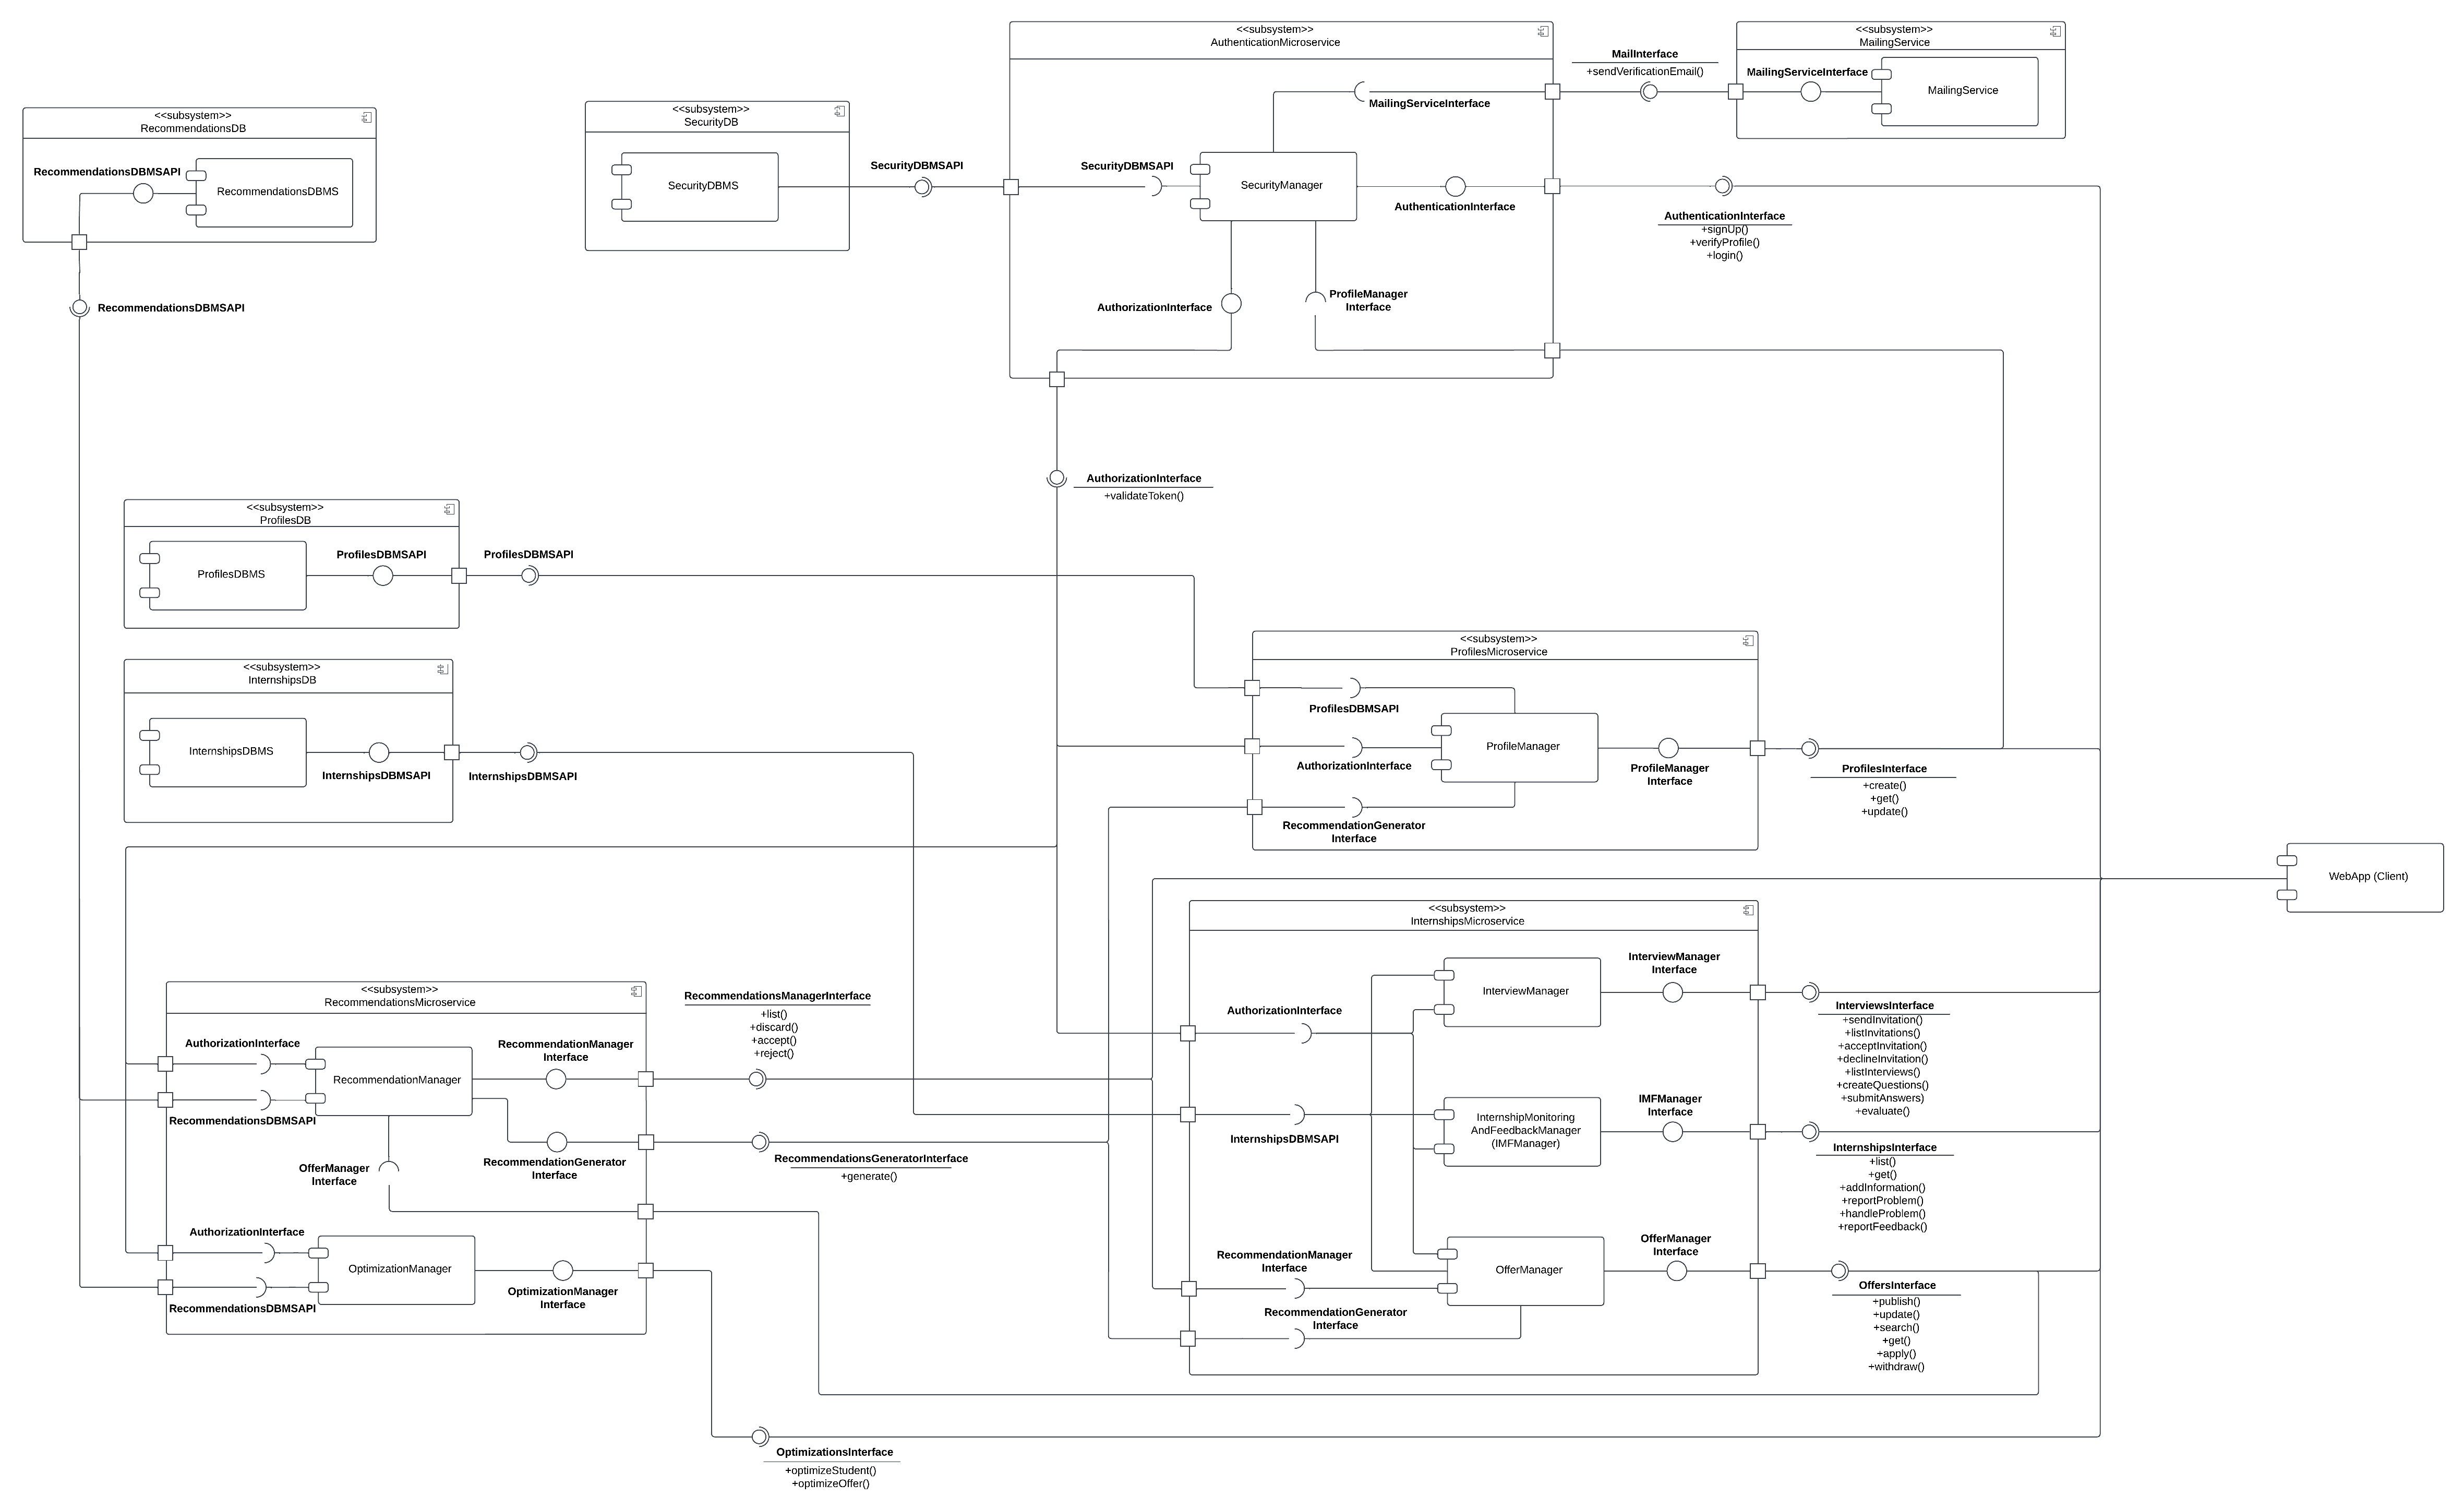
\includegraphics[width=0.95\linewidth]{LaTeXCode/images/ComponentDiagram/component_view.png}
        \caption{Component diagram of the S\&C system.}
        \label{fig:component_diagram}
    \end{center}
\end{figure}

\subsection{Components Description}
\label{subsec:components_description}

Each of the following components shall be thought of as a collection of simpler units that closely interact together to provide the offered functionalities. Specification of these units and how they form the component as a whole is left to the single teams or developers, as it is not binding towards the overall architecture of the system (given that every component must still fulfill the outlined expectations).

\begin{enumerate}
    \item \textbf{SecurityManager:} This component handles user authentication and registration processes for Students, Companies, and Universities. It manages the creation of new accounts by validating the provided information and communicating with the ProfileManager, and it also interacts with the MailingService to verify user identities. Additionally, it manages secure login operations, ensuring that only authenticated users can access the platform, and is used by other components to verify that users have the necessary authorization to execute the incoming requests.
    \item \textbf{MailingService:} This component handles the email communications needed for the ongoing account verification processes. It implements the mail server functionalities needed to send verification emails to users during the sign-up phase, each containing a link that shall be clicked to complete the registration process.
    \item \textbf{ProfileManager:} This component handles the operations required to view and update user profiles. For students, sign-ups or updates to relevant details initiate the generation of new recommendations by interacting with the RecommendationManager, aimed either at them or at some Companies, ensuring they both remain aligned with current opportunities.
    \item \textbf{OfferManager:} This component manages the lifecycle of internship offers within the platform. It provides companies with tools to create, update, withdraw and manage their internship announcements. When creating an offer, the OfferManager automatically extracts the relevant keywords to be applied to the offer from the description provided. The component also integrates advanced filtering mechanisms to allow students to search efficiently for relevant opportunities and view them. Moreover, the OfferManager facilitates interactions between students and companies by managing applications and allowing them to keep the status of offers up-to-date. As for the ProfileManager, this component interacts with the RecommendationManager to generate new recommendations when creating or updating relevant details of offers.
    \item \textbf{InterviewManager:} This component facilitates and manages the whole interview process between students and companies. It provides tools for scheduling, conducting, monitoring and evaluating interviews. The component ensures easy communication between the parties and handles the creation, delivery and management of interview invitations. Additionally, it records evaluations and updates the status of candidates in the selection process, easing the transition from interviews to final decisions.
    \item \textbf{InternshipMonitoringAndFeedbackManager (IMFM):} This component manages the monitoring, complaining and feedback processes for internships. It enables students and companies to provide updates and view detailed information about ongoing internships they are participating in. It also allows parties to report issues encountered during internships, forwarding these reports to the university for resolution. At the conclusion of an internship, the component facilitates the collection of feedback from both students and companies, so that this information can be used in the future to enhance the recommendation algorithms and ensure a continuous improvement of the system.
    \item \textbf{RecommendationManager:} This component handles the operations needed to generate and manage recommendations. It identifies internship recommendations for students and student recommendations for companies by performing graph analyses on a graph database storing the relationships between students, companies, offers, skills and various feedback expressed through time: specifically, the RecommendationManager detects links between the keywords associated with students' resumes and offers published, and can also perform more complex queries which statistically identify relationships between profiles, preferences and past histories of all users on the platform, by means of collaborative filtering and content-based filtering. Last, but not least, this component also allows both of them to view and act on their received recommendations.
    \item \textbf{OptimizationManager:} This component manages the operations needed to generate personalized suggestions to improve user content. It relies on a Large Language Model (LLM) that has been properly fine-tuned to identify enhancements to be applied to students' profiles and offers' descriptions to make them more appealing and increase their chances of being selected. The OptimizationManager also takes into account the opportunities (students and offers) currently available on the platform by feeding to the LLM some aggregated data resulting from whole-graph analyses, so that it can provide suggestions that are customized for the current situation.
    \item \textbf{SecurityDBMS, ProfilesDBMS, InternshipsDBMS:} relational DBMSs that store data respectively about account credentials, profiles information and internship information.
    \item \textbf{RecommendationsDBMS:} graph DBMS that stores data about the relationships between users, skills, internships, recommendations and useful feedback in order to identify new recommendations by simple skill keyword searching or statistical whole-graph analyses.
\end{enumerate}

\newpage

\section{Deployment View}
\label{sec: deployment_view}

The system is deployed as a distributed microservices architecture leveraging containerization and orchestration to achieve high scalability, resiliency and modularity. Each layer has distinct responsibilities and is deployed across a collection of servers to guarantee replication and fault tolerance.

\begin{itemize}
    \item \textbf{Presentation Layer:} represents the client in a traditional client-server architecture. Users interact with the system via a web application running in their browser.
    \item \textbf{Application Layer:} hosts containerized microservices that provide all business functionalities.
    The deployment diagram illustrates a possible allocation of these containers across the servers available to this layer. The actual number of microservice instances and their distribution during runtime are dynamically determined by the container orchestration platform based on workload demands. This ensures optimal resource utilization and adaptability to varying request volumes.
    \item \textbf{Service Management Layer:} responsible for managing the orchestration of microservices and auxiliary services. This layer includes the mailing service used during the registration process, the Data Layer Load Balancer, which manages the distribution of requests to database replicas in the Data Layer, and the Replication-Consistency Middleware, which handles data replication and consistency.
    \item \textbf{Data Layer:} manages persistent data storage using replicated databases to ensure fault tolerance and performance optimization. Data replicas are statically allocated, in order to implement strategic business decisions about scalability and geographic allocation manually, and the load balancer in the Service Management Layer ensures requests are distributed evenly across these replicas.
\end{itemize}

Communication between the components relies on REST APIs (HTTPS), with TCP/IP for lower-level communication, especially with the Service Management Layer and with the Data Layer.

\begin{figure} [H]
    \begin{center}
        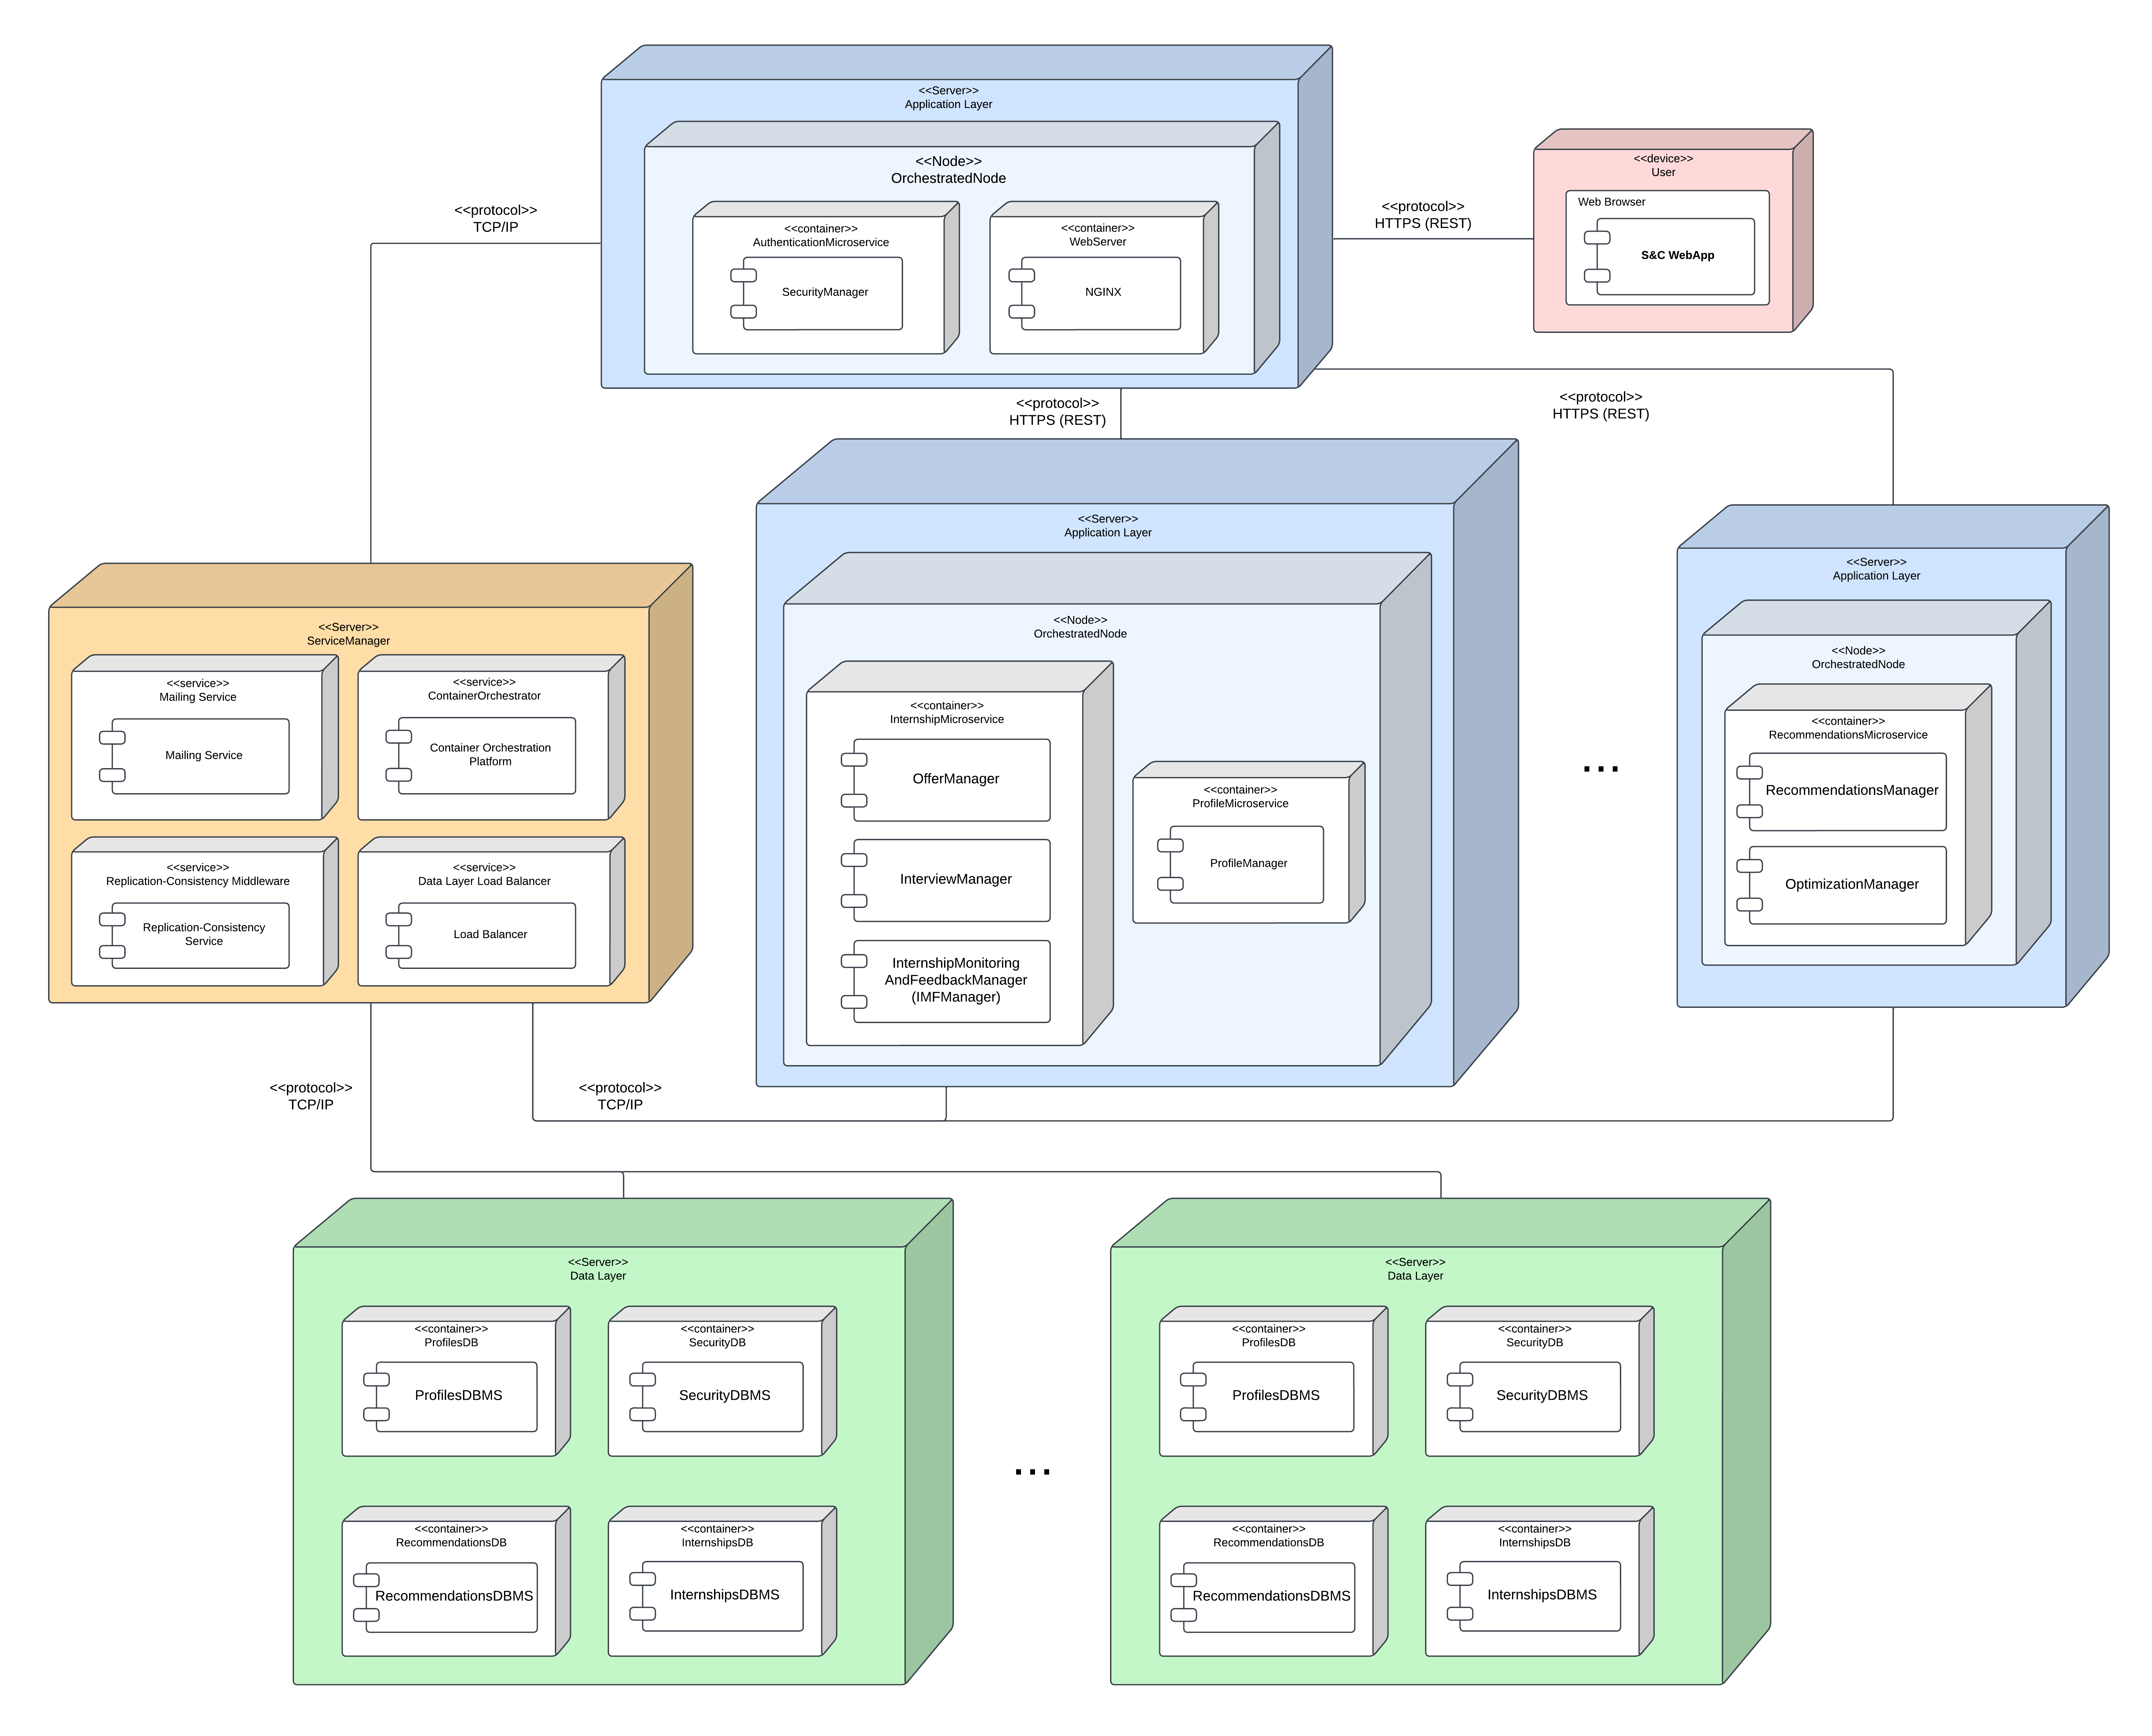
\includegraphics[width=0.95\linewidth]{LaTeXCode/images/DeploymentDiagram/deployment_view.png}
        \caption{UML Deployment Diagram.}
        \label{fig: deployment_diagram}
    \end{center}
\end{figure}

\subsection{Detailed Layer Decisions}
\label{subsec: layer_description}

\paragraph{Web Server}
The entry point of the application is NGINX, a web server deployed in a container acting as a reverse proxy, hosting all API endpoints, acting as an API Gateway and forwarding the requests from the user layer to the appropriate microservices in the application layer. 
The component gatekeeps all traffic to microservices and collaborates with the SecurityManager in order to provide authentication and authorization mechanisms.
Internally, it also performs load balancing of the incoming requests and URL rewriting a redirection. 
It simplifies routing logic and improves the security of the system by exposing a single public endpoint.

\paragraph{Scalability}
Each microservice and DBMS runs in an isolated container, enabling independent scaling. The container orchestrator dynamically adjusts the number of containers based on resource consumption or incoming traffic, and replication in the Data Layer improves read performance by distributing queries across replicas.

\paragraph{Resiliency}
The container orchestration platform manages failover and automatically restarts containers in case of crashes.
Data replication ensures availability, even in the event of server failure and the Data Layer Load Balancer prevents overloading by evenly distributing requests.

\paragraph{Orchestration Platform Considerations}
A specific Container Orchestration Technology is not specified, even if ideally it would be preferable to use Kubernetes and deploy the containers with Docker, since they are the most widely adopted platforms and are well known to system administrators, simplifying their use for all the people involved in deploying and managing the infrastructure.
In particular, the orchestrator offers many useful functionalities in the context of our architecture, such as automatic scaling, monitoring, networking and server-side service discovery, lightening the burden of managing such aspects.
In the server-side discovery method, services are registered with an API server (if Kubernetes is chosen, called Kubernetes API Server), which acts as a central registry for services. Clients then query the API server to discover the available services, which are dynamically deployed and for this reason real addresses may change. The API server responds with a list of available microservices and their corresponding endpoints. When the reverse proxy makes a network request for a service, the Orchestration Platform routes the request to the appropriate endpoint using the information stored. While doing this, the orchestration platform also manages load balancing among the available microservices.

\paragraph{Replication and Data Consistency}
The Data Layer adopts a Multi-Leader Replication protocol to maintain consistency across replicas, accommodating the geographical distribution of data nodes. This approach enables multiple leaders to handle write operations concurrently, reducing latency and ensuring high availability.
In this setup, write operations can be performed on any leader node. Changes are then propagated asynchronously to other leaders and replicas, ensuring eventual consistency across the system.
Read operations are distributed across multiple replicas to optimize performance and handle high query volumes effectively.
This replication model provides enhanced fault tolerance, as the failure of a single leader does not disrupt write operations. However, potential conflicts from concurrent writes have to be managed using conflict resolution strategies, ensuring data integrity across all replicas.

\newpage

\section{Component Interfaces}
\label{sec: component_interfaces}
In this section the component interfaces defined are described, highlighting for each one the expected inputs and outputs.

\subsection{REST API Endpoints}
Each microservice of the system exposes one or more interfaces, which are the resource endpoints of the defined REST API. The Service Orchestrator is responsible for carrying out the Service Discovery process among the physical servers, as it is the one that knows how microservices are deployed on the different machines at every instant, and can thus route the requests aimed at the specific resources to the correct location for the corresponding microservice.
The structure of an API request directed to a microservice of the system must adhere to the following structure:

\texttt{https://DOMAIN/api/VERSION/INTERFACE/FUNCTION}

In particular:
\begin{itemize}
    \item The communication protocol must be HTTPS.
    \item \texttt{DOMAIN} is the domain name of the S\&C system.
    \item \texttt{/api/} is just syntactic sugar to highlight that the request is aimed at an API resource.
    \item \texttt{VERSION} is the version of the API to be addressed (for compatibility purposes).
    \item \texttt{INTERFACE} is the first-level hierarchy, indicating the specific interface to be addressed (not the actual microservices, as they could expose more than one interface): every interface keeps the same name indicated in the Component View in \hyperref[fig:component_diagram]{\protect\uline{Section 2.2.1}}, but without the final "Interface" keyword.
    \item \texttt{FUNCTION} is the API procedure of the specified interface that is being requested.
\end{itemize}

The following is a list of all the API endpoints, grouped by interface: for each one, the expected input parameters, responses\footnote{Both here and in the Sequence Diagrams in \hyperref[sec:runtime_view]{\protect\uline{Section 2.5}}, all \textbf{400 Bad Request} responses for requests about nonexisting resources (such as invalid IDs) are omitted for brevity. The same goes for \textbf{401 Unauthorized} responses, generated and forwarded by the SecurityManager upon denial resulting from calls to its \texttt{/validateToken} endpoint: even if omitted at the moment, such calls shall be present in the implementation code whenever a request that involves access to any protected resource is received and whenever access authorization of the requestor needs to be verified.} (with eventual important headers), and output values are listed. For additional security, the endpoints must always be invoked through the HTTPS POST method: input parameters and eventual output values are always provided respectively in the body of the request and the response, and both must be in standard JSON format.

\subsubsection*{/authentication}
\begin{itemize}
    \item \texttt{/signUp} \\
        \textit{parameters:} \{ email: String, password: String, accountType: Enum(Student, Company, University) \} \\
        \textit{responses:}
        \begin{itemize}
            \item \textbf{303 See Other:} \\ 
            header: "Location: loginPage", \\
            body: \{ cause: Enum(alreadyRegistered, emailSent) \}
            \item \textbf{400 Bad Request:} \\
            body: \{ error: Enum(missingFields, invalidPassword) \}
        \end{itemize}
    \item \texttt{/verifyProfile}\footnote{As an exception, this is the only endpoint to be accessed through a GET request, as it is intended to be invoked by clicking the link in the verification email.} \\
        \textit{parameters:} \{ userID: int \} \\
        \textit{responses:} 
        \begin{itemize}
            \item \textbf{308 Permanent Redirect:} \\
            header: "Location: updateProfilePage" \\
            body: \{ cause: Enum(profileVerified) \}
        \end{itemize}
    \item \texttt{/login} \\
        \textit{parameters:} \{ username: String, password: String \footnote{Note that it is not the actual password, but only its hash value.} \}\\
        \textit{responses:}
        \begin{itemize}
            \item \textbf{308 Permanent Redirect:} \\
            header: "Location: dashboardPage" \\
            body: \{ cause: Enum(successfulLogin), token: String \}
            \item \textbf{308 Permanent Redirect:} \\
            header: "Location: updateProfilePage" \\
            body: \{ cause: Enum(incompleteProfile), token: String \}
            \item \textbf{400 Bad Request:} \\
            body: \{ error: Enum(wrongCredentials, unverifiedAccount) \}
        \end{itemize}
\end{itemize}

\subsubsection*{/mail}
\begin{itemize}
    \item \texttt{/sendVerificationEmail} \\
        \textit{parameters:} \{ email: String, confirmationLink: String \} \\
        \textit{responses:}
        \begin{itemize}
            \item \textbf{204 No Content}
        \end{itemize}
\end{itemize}

\subsubsection*{/authorization}
\begin{itemize}
    \item \texttt{/validateToken} \\
        \textit{parameters:} \{ token : String \} \\
        \textit{responses:}
        \begin{itemize}
            \item \textbf{200 OK:} \\
            body: \{ authorized: true \}
            \item \textbf{401 Unauthorized:} \\
            body: \{ authorized: false \}
        \end{itemize}
\end{itemize}

\subsubsection*{/profiles}
\begin{itemize}
    \item \texttt{/create} \\
        \textit{parameters:} \{ userID: int, user: User \} \\
        \textit{responses:}
        \begin{itemize}
            \item \textbf{204 No Content}
        \end{itemize}
    \item \texttt{/get} \\
        \textit{parameters:} \{ userID: int \} \\
        \textit{responses:}
        \begin{itemize}
            \item \textbf{200 OK:} \\
            body: \{ user: User \}
            \item \textbf{400 Bad Request:} \\
            body: \{ cause: Enum(invalidUser) \}
        \end{itemize}
    \item \texttt{/update} \\
        \textit{parameters:} \{ userID: int, user: User \} \\
        \textit{responses:}
        \begin{itemize}
            \item \textbf{200 OK:} \\
            body: \{ popup: Enum(profileUpdated), user: User \}
            \item \textbf{400 Bad Request:} \\
            body: \{ cause: Enum(missingFields) \}
        \end{itemize}
\end{itemize}

\subsubsection*{/offers}
\begin{itemize}
    \item \texttt{/publish} \\
        \textit{parameters:} \{ companyID: int, offer: Offer \} \\
        \textit{responses:}
        \begin{itemize}
            \item \textbf{307 Temporary Redirect:} \\
            header: "Location: offerPage" \\
            body: \{ popup: Enum(offerPublished), offerID: int \}
            \item \textbf{400 Bad Request:} \\
            body: \{ cause: Enum(missingFields, nonCompliantInformation) \}
        \end{itemize}
    \item \texttt{/update} \\
        \textit{parameters:} \{ companyID: int, offerID: int, offer: Offer \} \\
        \textit{responses:}
        \begin{itemize}
            \item \textbf{200 OK:} \\
            body:  \{ popup: Enum(offerUpdated), offer: Offer \}
            \item \textbf{400 Bad Request:} \\
            body: \{ cause: Enum(missingFields, nonCompliantInformation) \}
        \end{itemize}
    \item \texttt{/search} \\
        \textit{parameters:} \{ filters: [ filter: Filter ] \} \\
        \textit{responses:}
        \begin{itemize}
            \item \textbf{200 OK:} \\
            body: \{ offersList: [ offer: Offer ] \}
        \end{itemize}
    \item \texttt{/get} \\
        \textit{parameters:} \{ offerID: int \} \\
        \textit{responses:}
        \begin{itemize}
            \item \textbf{200 OK:} \\
            body: \{ offer: Offer \}
        \end{itemize}
    \item \texttt{/apply} \\
        \textit{parameters:} \{ studentID: int, offerID: int \} \\
        \textit{responses:}
        \begin{itemize}
            \item \textbf{200 OK:} \\
            body: \{ popup: Enum(applicationSubmitted) \}
            \item \textbf{400 Bad Request:} \\
            body: \{ cause: Enum(expiredDeadline) \}
        \end{itemize}
    \item \texttt{/withdraw} \\
        \textit{parameters:} \{ companyID: int, offerID: int \} \\
        \textit{responses:}
        \begin{itemize}
            \item \textbf{308 Permanent Redirect:} \\
            header: "Location: dashboardPage" \\
            body: \{ cause: Enum(successfulWithdrawal) \}
        \end{itemize}
\end{itemize}

\subsubsection*{/interviews}
\begin{itemize}
    \item \texttt{/sendInvitation} \\
        \textit{parameters:} \{ studentID: int, offerID: int, date: DateTime, type: Enum(inPerson, inPlatform), otherDetails: String \} \\
        \textit{responses:}
        \begin{itemize}
            \item \textbf{200 OK:} \\
            body: \{ popup: Enum(invitationSent) \}
        \end{itemize}
    \item \texttt{/listInvitations} \\
        \textit{parameters:} \{ userID: int\} \\
        \textit{responses:}
        \begin{itemize}
            \item \textbf{200 OK:} \\
            body: [ \{ offerID: int, offer: Offer, date: DateTime, type: Enum(inPerson, inPlatform), otherDetails: String \} ]
        \end{itemize}
    \item \texttt{/acceptInvitation} \\
        \textit{parameters:} \{ offerID: int, studentID: int \} \\
        \textit{responses:}
        \begin{itemize}
            \item \textbf{200 OK:} \\
            body: \{ popup: Enum(invitationAccepted) \}
        \end{itemize}
    \item \texttt{/declineInvitation} \\
        \textit{parameters:} \{ offerID: int, studentID: int, reason: String \} \\
        \textit{responses:}
        \begin{itemize}
            \item \textbf{200 OK:} \\
            body: \{ popup: Enum(invitationDeclined) \}
        \end{itemize}
    \item \texttt{/listInterviews} \\
        \textit{parameters:} \{ userID: int\} \\
        \textit{responses:}
        \begin{itemize}
            \item \textbf{200 OK:} \\
            body: [ \{ interviewID: int, interview: Interview \} ]
        \end{itemize}
    \item \texttt{/createQuestions} \\
        \textit{parameters:} \{ companyID: int, interviewsIDs: [ interviewID: int ], questions: [ content : String ] \} \\
        \textit{responses:}
        \begin{itemize}
            \item \textbf{200 OK:} \\
            body: \{ popup: Enum(questionsCreated), questions: [ \{ questionIDs: int, question: Question \} ] \}
        \end{itemize}
    \item \texttt{/submitAnswer} \\
        \textit{parameters:} \{ studentID: int, interviewID: int, questionID: int,  answer: String \} \\
        \textit{responses:}
        \begin{itemize}
            \item \textbf{200 OK:} \\
            body: \{ popup: Enum(answerSubmitted), answer: Answer \}
        \end{itemize}
    \item \texttt{/evaluate} \\
        \textit{parameters:} \{ studentID: int, offerID: int, status: Enum(Selected, Rejected), feedback: String \} \\
        \textit{responses:}
        \begin{itemize}
            \item \textbf{200 OK:} \\
            body: \{ popup: Enum(interviewEvaluated) \}
        \end{itemize}
\end{itemize}

\subsubsection*{/internships}
\begin{itemize}
    \item \texttt{/list} \\
        \textit{parameters:} \{ userID: int \} \\
        \textit{responses:}
        \begin{itemize}
            \item \textbf{200 OK:} \\
            body: [ \{ internshipID: int, internship: Internship \} ]
        \end{itemize}
    \item \texttt{/get} \\
        \textit{parameters:} \{ internshipID: int, userID: int \} \\
        \textit{responses:}
        \begin{itemize}
            \item \textbf{200 OK:} \\
            body: \{ internship: Internship \}
        \end{itemize}
    \item \texttt{/addInformation} \\
        \textit{parameters:} \{ internshipID: int, userID: int, information: String \} \\
        \textit{responses:}
        \begin{itemize}
            \item \textbf{200 OK:} \\
            body: \{ popup: Enum(informationAdded) \}
        \end{itemize}
    \item \texttt{/reportProblem} \\
        \textit{parameters:} \{ internshipID: int, userID: int, problem: String \} \\
        \textit{responses:}
        \begin{itemize}
            \item \textbf{200 OK:} \\
            body: \{ popup: Enum(problemReported) \}
            \item \textbf{400 Bad Request:} \\
            body: \{ cause: Enum(missingFields) \}
        \end{itemize}
    \item \texttt{/handleProblem} \\
        \textit{parameters:} \{ internshipID: int, problemID: int, status: Enum(Unhandled, In Progress, Solved, Hidden) \} \\
        \textit{responses:}
        \begin{itemize}
            \item \textbf{200 OK:} \\
            body: \{ popup: Enum(statusUpdated), problemID: int, status: Enum(Unhandled, In Progress, Solved, Hidden) \}
        \end{itemize}
    \item \texttt{/reportFeedback} \\
        \textit{parameters:} \{ internshipID: int, userID: int, feedback: String \} \\
        \textit{responses:}
        \begin{itemize}
        \item \textbf{200 OK:} \\
            body: \{ popup: Enum(feedbackReported) \}
        \end{itemize}
\end{itemize}

\newpage

\subsubsection*{/recommendations/generator}
\begin{itemize}
    \item \texttt{/generate}\footnote{Calls to this API endpoint are overloaded, as the new or updated Student or Offer needs to be sent to the RecommendationManager, because changes might still not have been recorded in the RecommendationsDBMS because of eventual consistency.} \\
        \textit{parameters:} \{ studentID: int, student: Student \} \\
        \textit{responses:}
        \begin{itemize}
            \item \textbf{204 No Content}
        \end{itemize}
    \item \texttt{/generate}$^4$ \\
        \textit{parameters:} \{ offerID: int, offer: Offer \} \\
        \textit{responses:}
        \begin{itemize}
            \item \textbf{204 No Content}
        \end{itemize}
\end{itemize}

\subsubsection*{/recommendations/manager}
\begin{itemize}
    \item \texttt{/list} \\
        \textit{parameters:} \{ userID: int \} \\
        \textit{responses:}
        \begin{itemize}
            \item \textbf{200 OK:} \\
            body: \{ listOfRecommendations: [ recommendation: Recommendation ] \}
        \end{itemize}
    \item \texttt{/discard} \\
        \textit{parameters:} [ recommendationID: int ] \\
        \textit{responses:}
        \begin{itemize}
            \item \textbf{200 OK:} \\
            body: \{ popup: Enum(successfullyDiscarded) \}
        \end{itemize}
    \item \texttt{/accept} \\
        \textit{parameters:} [ recommendationID: int ] \\
        \textit{responses:}
        \begin{itemize}
            \item \textbf{200 OK:} \\
            body: \{ popup: Enum(successfullyAccepted) \}
        \end{itemize}
    \item \texttt{/reject} \\
        \textit{parameters:} [ recommendationID: int ] \\
        \textit{responses:}
        \begin{itemize}
            \item \textbf{200 OK:} \\
            body: \{ popup: Enum(successfullyRejected) \}
        \end{itemize}
\end{itemize}

\subsubsection*{/optimizations}
\begin{itemize}
    \item \texttt{/optimizeStudent} \\
        \textit{parameters:} \{ userID: int \} \\
        \textit{responses:}
        \begin{itemize}
            \item \textbf{200 OK:} \\
            body: \{ suggestedOptimizations: String \}
        \end{itemize}
    \item \texttt{/optimizeOffer} \\
        \textit{parameters:} \{ offerID: int \} \\
        \textit{responses:}
        \begin{itemize}
            \item \textbf{200 OK:} \\
            body: \{ suggestedOptimizations: String \}
        \end{itemize}
\end{itemize}

\subsection{Other Interfaces}

No additional interfaces are needed for the S\&C system, as no components inside a specific microservice ever need to communicate.

\newpage

\section{Runtime View}
\label{sec:runtime_view}%
In this section, the dynamic behavior of the S\&C system is portrayed. For each Use Case identified in Section 3.1 \textit{Use Cases and Activity Diagrams} of the RASD, the corresponding Sequence Diagram is provided, highlighting communication and messages exchanged between the components.
Once again, irrelevant details (such as: most client-side interactions between the User and the WebApp, e.g. form filling or negligible button clicking; call of most \texttt{get} functions of the API; extremely common operations such as calls to the \texttt{validateToken} function of the API) have been left out, as they would add further unnecessary complexity to the model, preventing a clear understanding of how components interact together.

\newcounter{uc}
\setcounter{uc}{1}
\newcommand{\cuc}{\theuc\stepcounter{uc}}

\subsubsection*{SD\cuc. Sign Up by a Student}
\label{subsubsec:signup_student_sd}
The Student clicks the "Sign Up" button on the sign up page and submits their data via the \texttt{.../api/v1/authentication/signUp/...} API endpoint. The request is forwarded to the \texttt{SecurityManager}, which validates the inputs and checks in the \texttt{SecurityDBMS} if the Student is already registered. If all checks succeed, it stores the Student data and calls the \texttt{MailingService} API to send a verification email to the specified email address through Simple Mail Transfer Protocol (SMTP). When the Student receives the email, if they click on the confirmation link within 24 hours, a call to the \texttt{.../api/v1/authentication/verifyProfile/...} API endpoint is made: the account is marked as verified in the \texttt{SecurityDBMS}, and the Student is redirected to the page for updating their profile, which takes place according to \hyperref[fig:update_profile_sd]{\protect\uline{SD5 - Update User Profile}}. If the timer for the verification instead expires, the account data is deleted from the \texttt{SecurityDBMS}.

\newpage

\begin{figure}[H]
    \begin{center}
         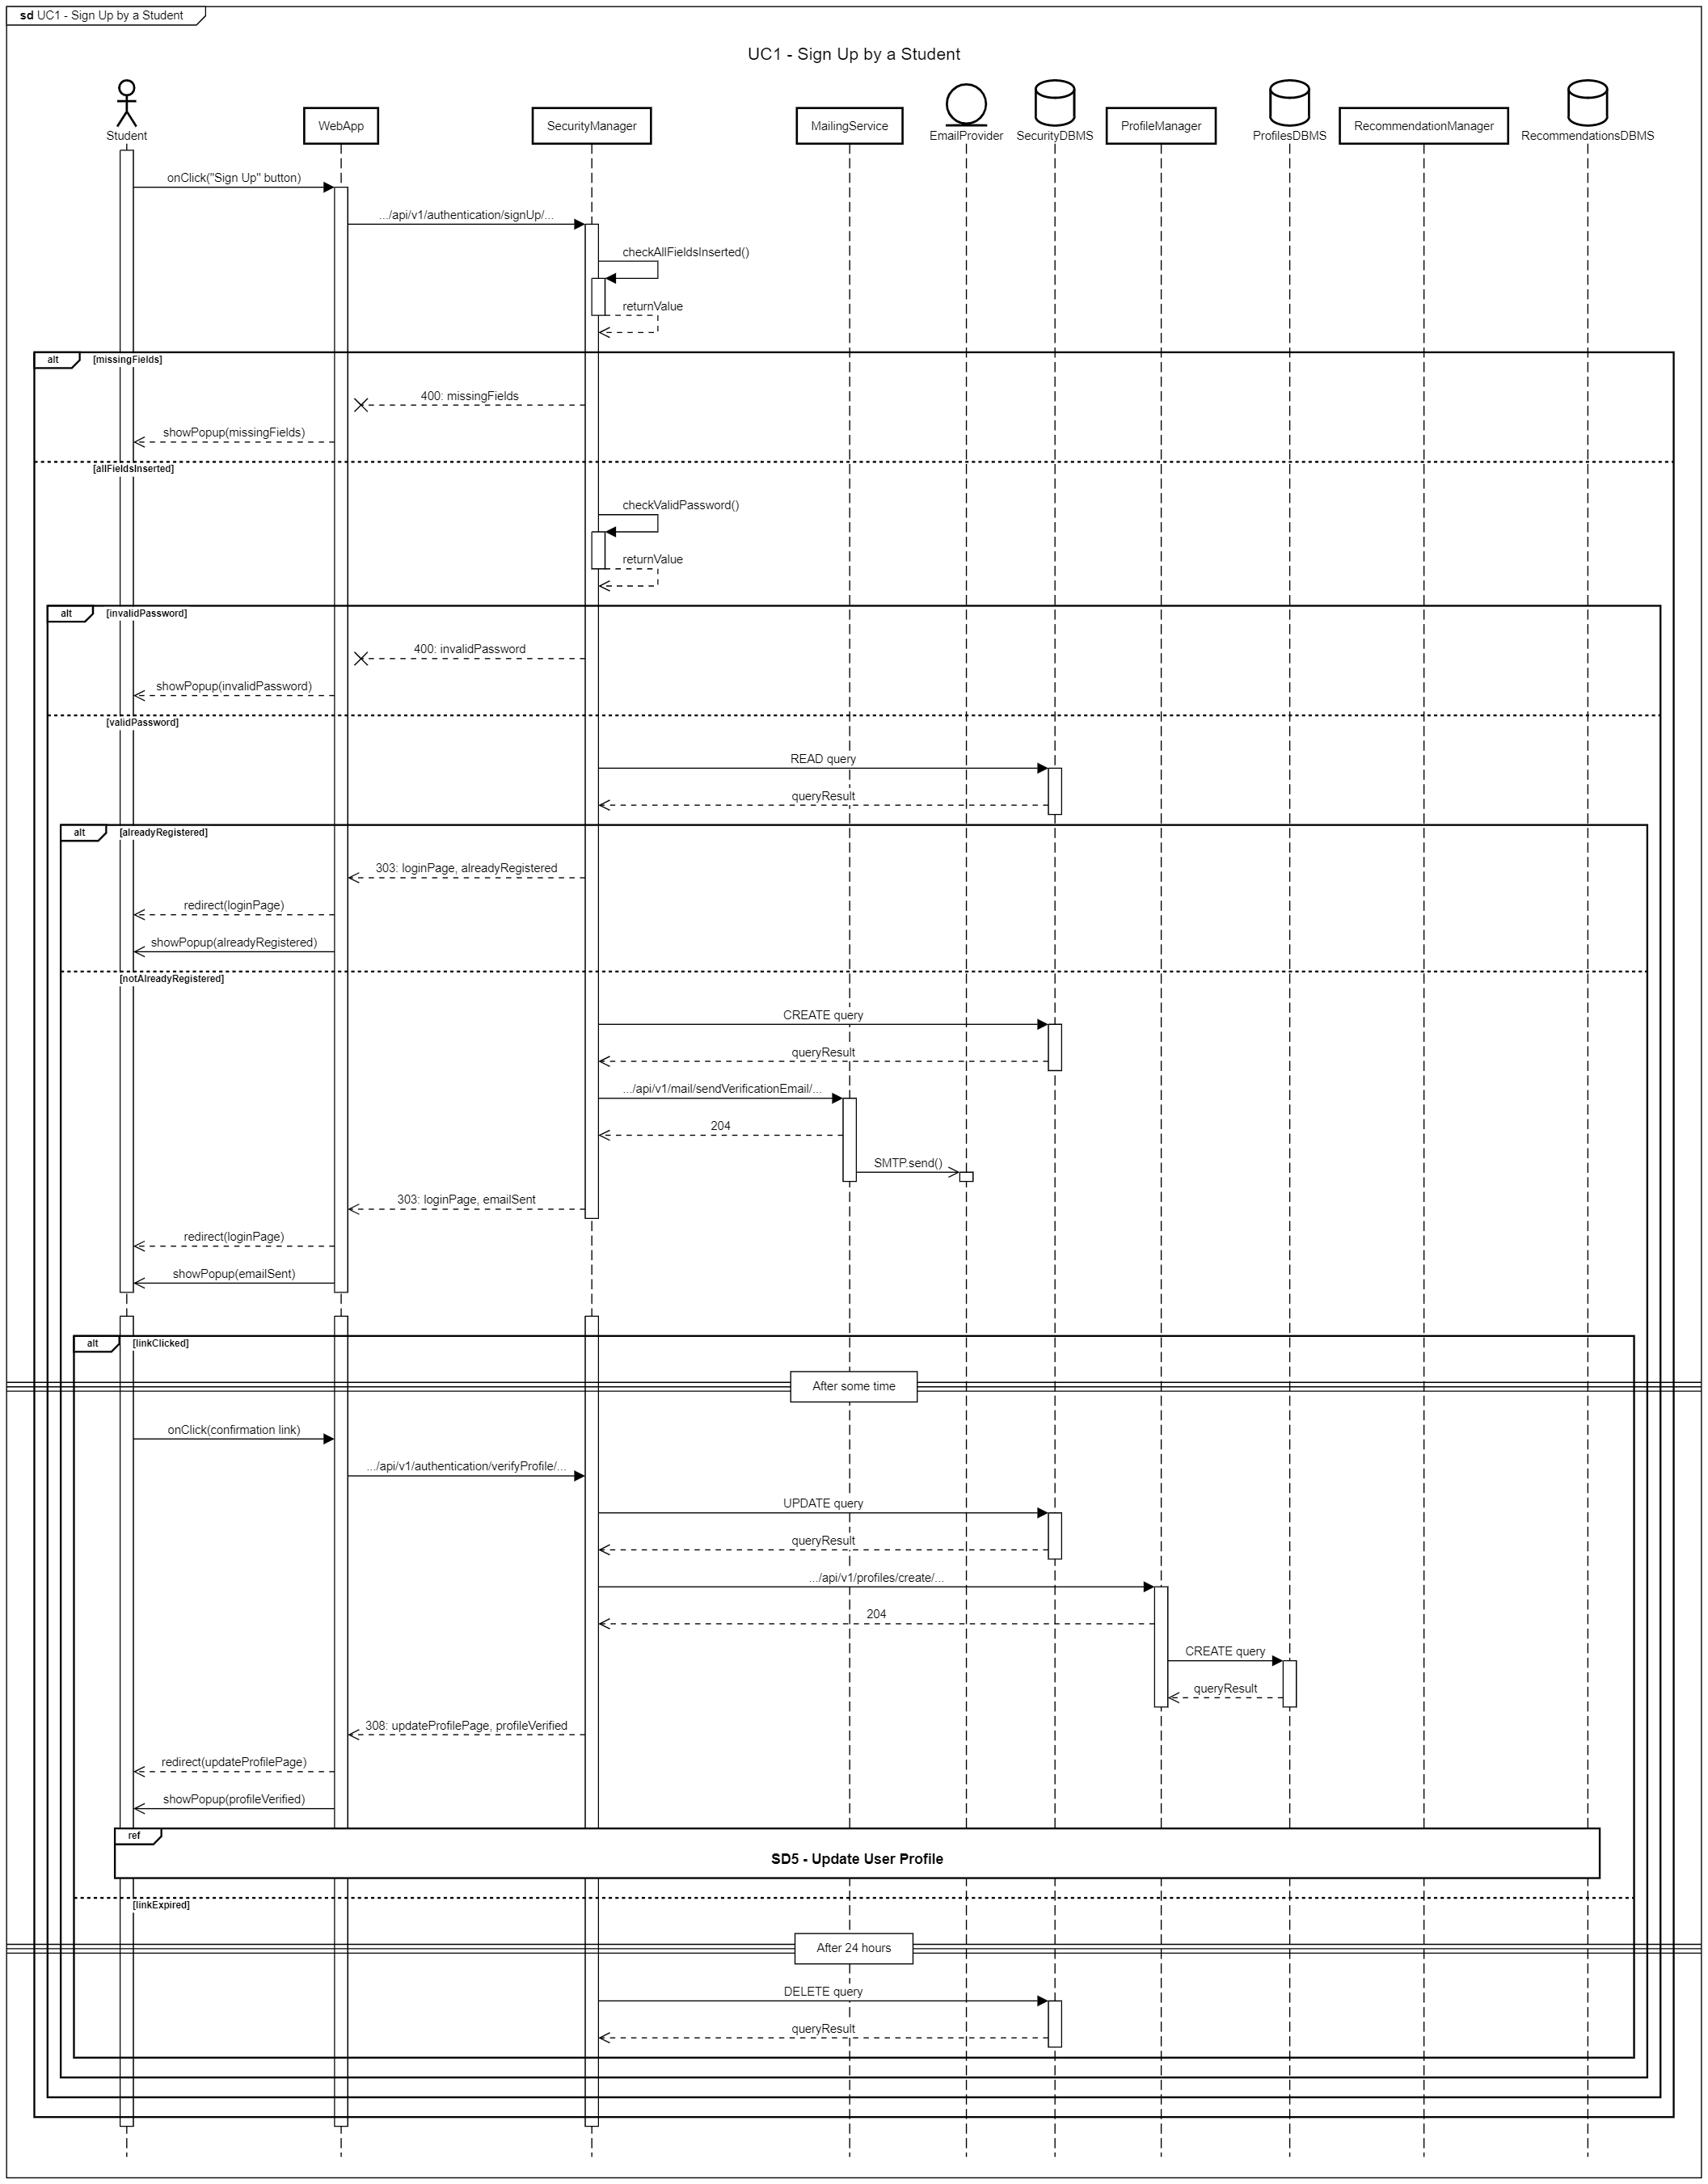
\includegraphics[width=1\linewidth]{LaTeXCode/images/SequenceDiagrams/UC1-sequenceDiagram.png}
         \caption{Sign Up by a Student}
         \label{fig:signup_student_sd}
     \end{center}
\end{figure}

\newpage

\subsubsection*{SD\cuc. Sign Up by a Company}
\label{subsubsec:signup_company_sd}
This Sequence Diagram is the same as the previous one, the only difference being that is is started by a Company and not by a Student.

\begin{figure}[H]
    \begin{center}
         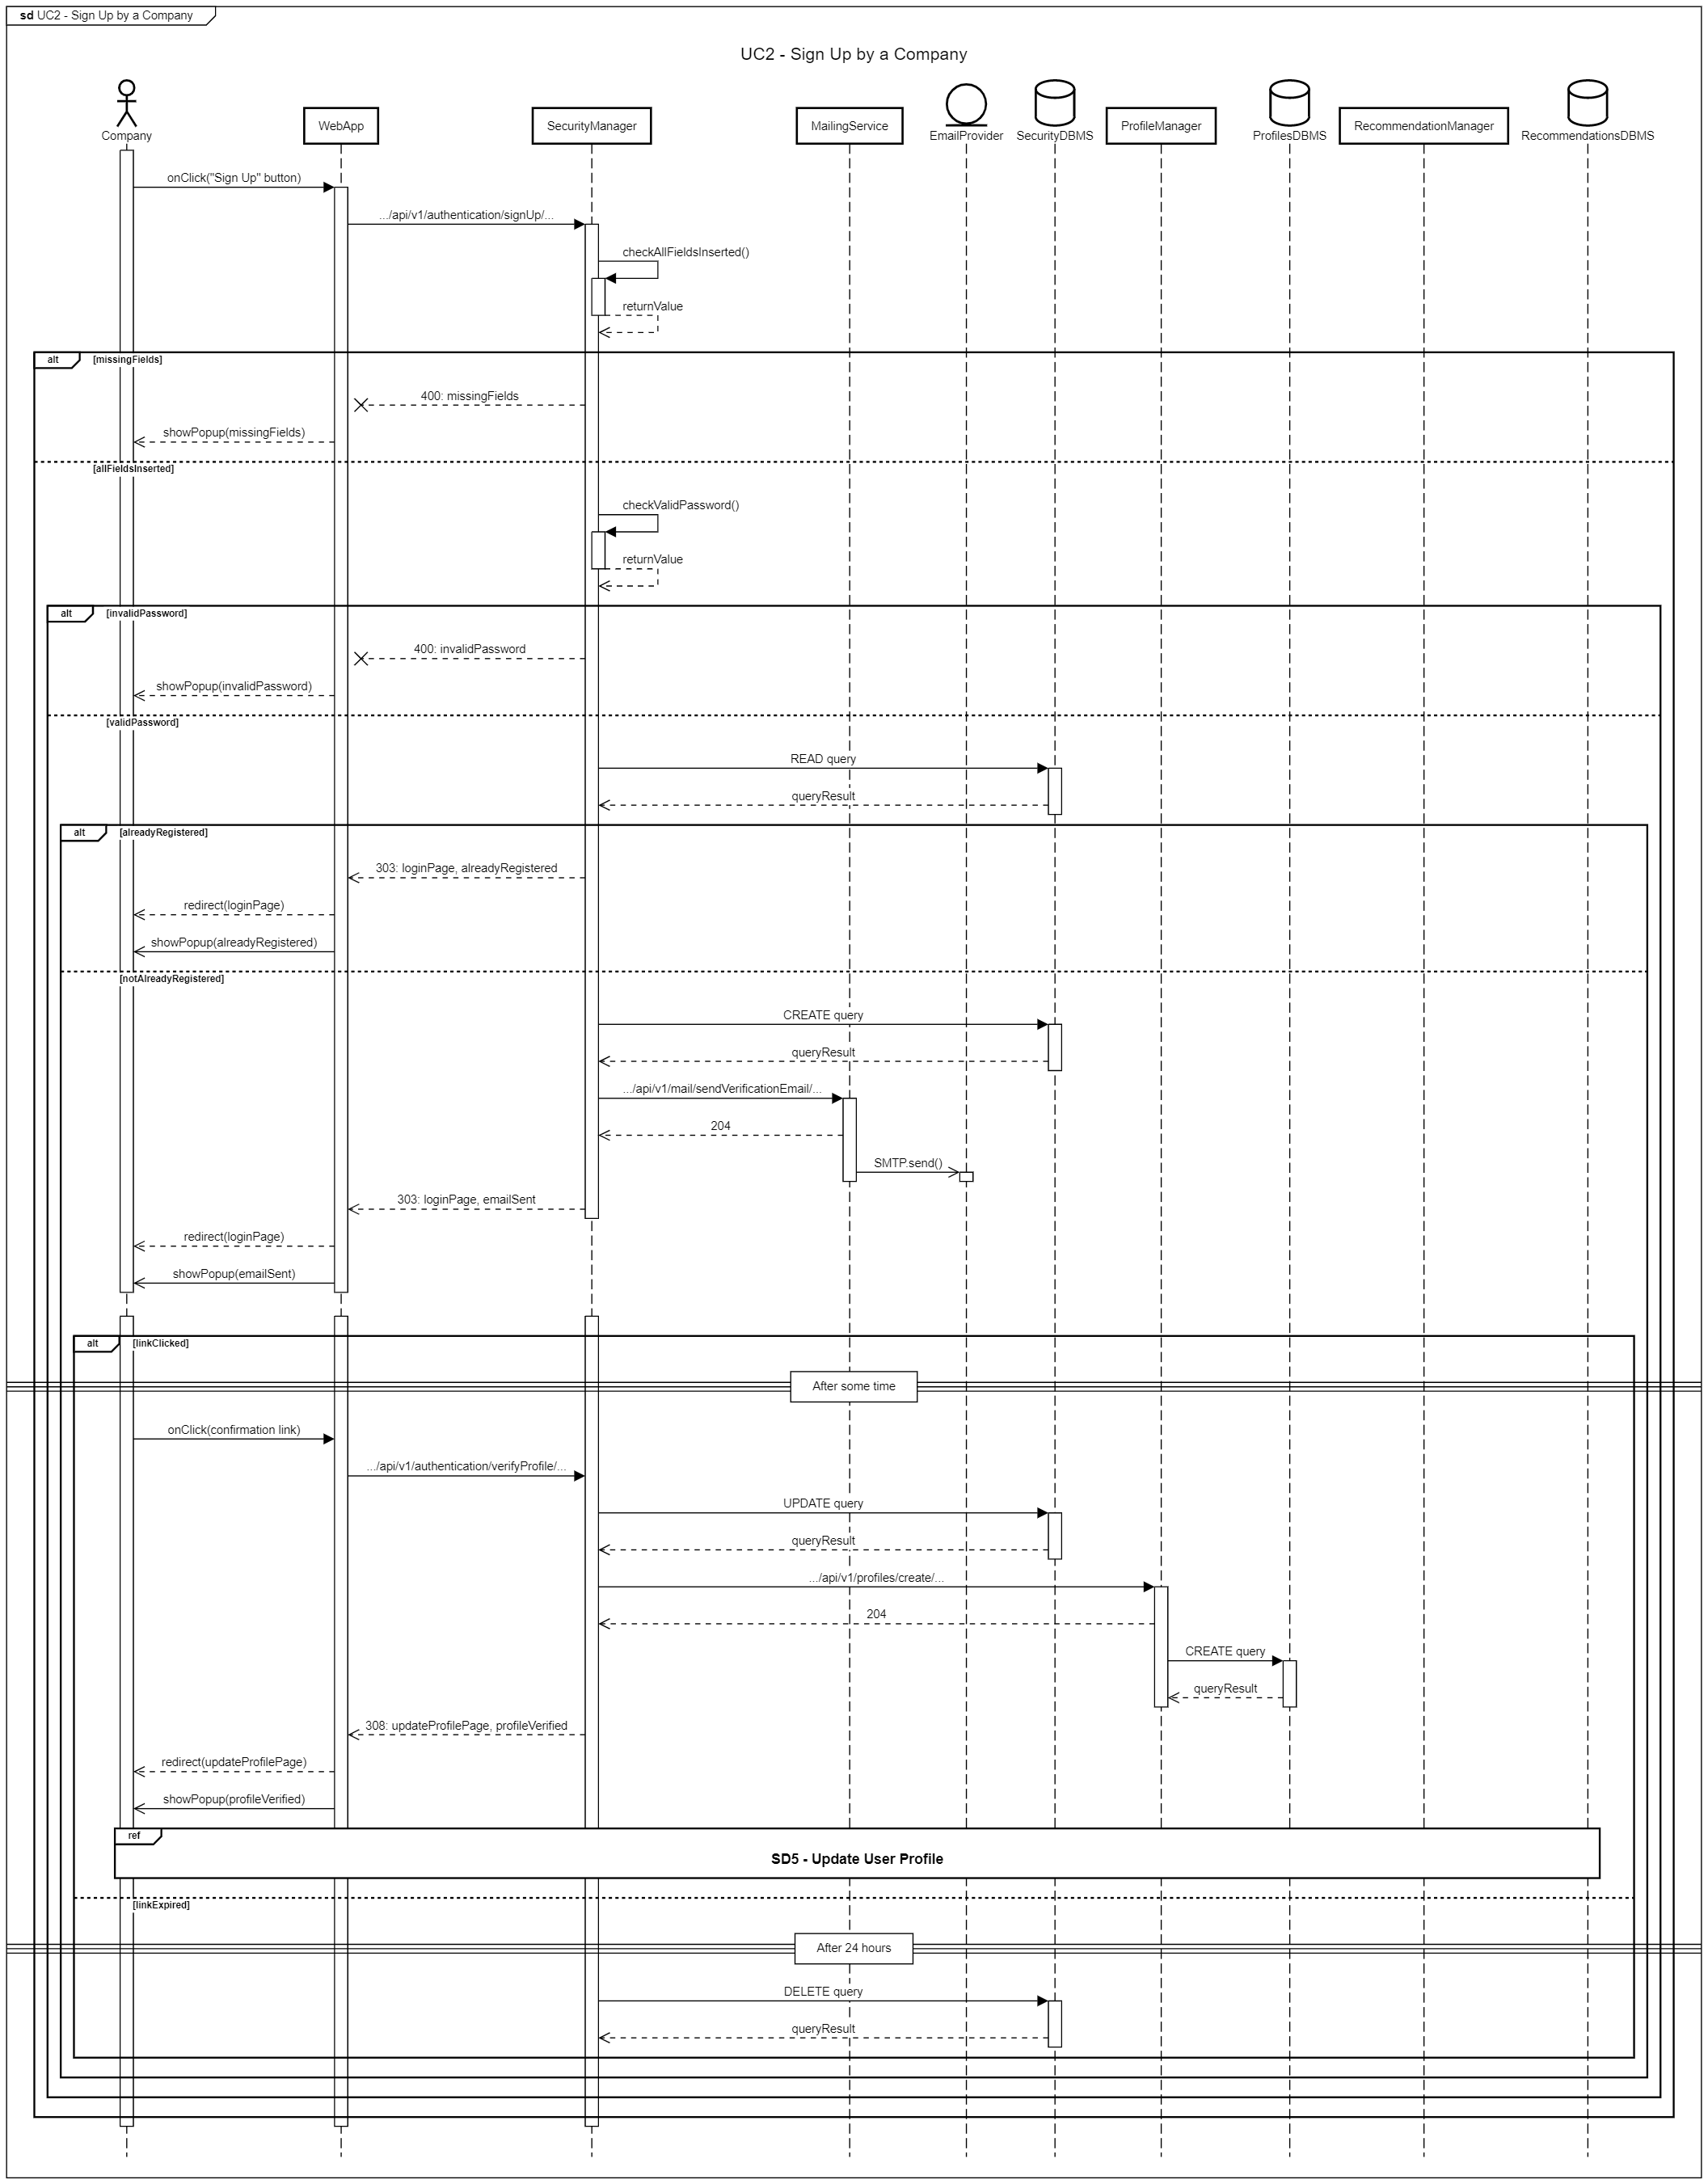
\includegraphics[width=0.9\linewidth]{LaTeXCode/images/SequenceDiagrams/UC2-sequenceDiagram.png}
         \caption{Sign Up by a Company}
         \label{fig:signup_company_sd}
     \end{center}
\end{figure}

\subsubsection*{SD\cuc. Sign Up by a University}
\label{subsubsec:signup_university_sd}
The same goes for this Sequence Diagram, which is in turn started by a University.

\begin{figure}[H]
    \begin{center}
         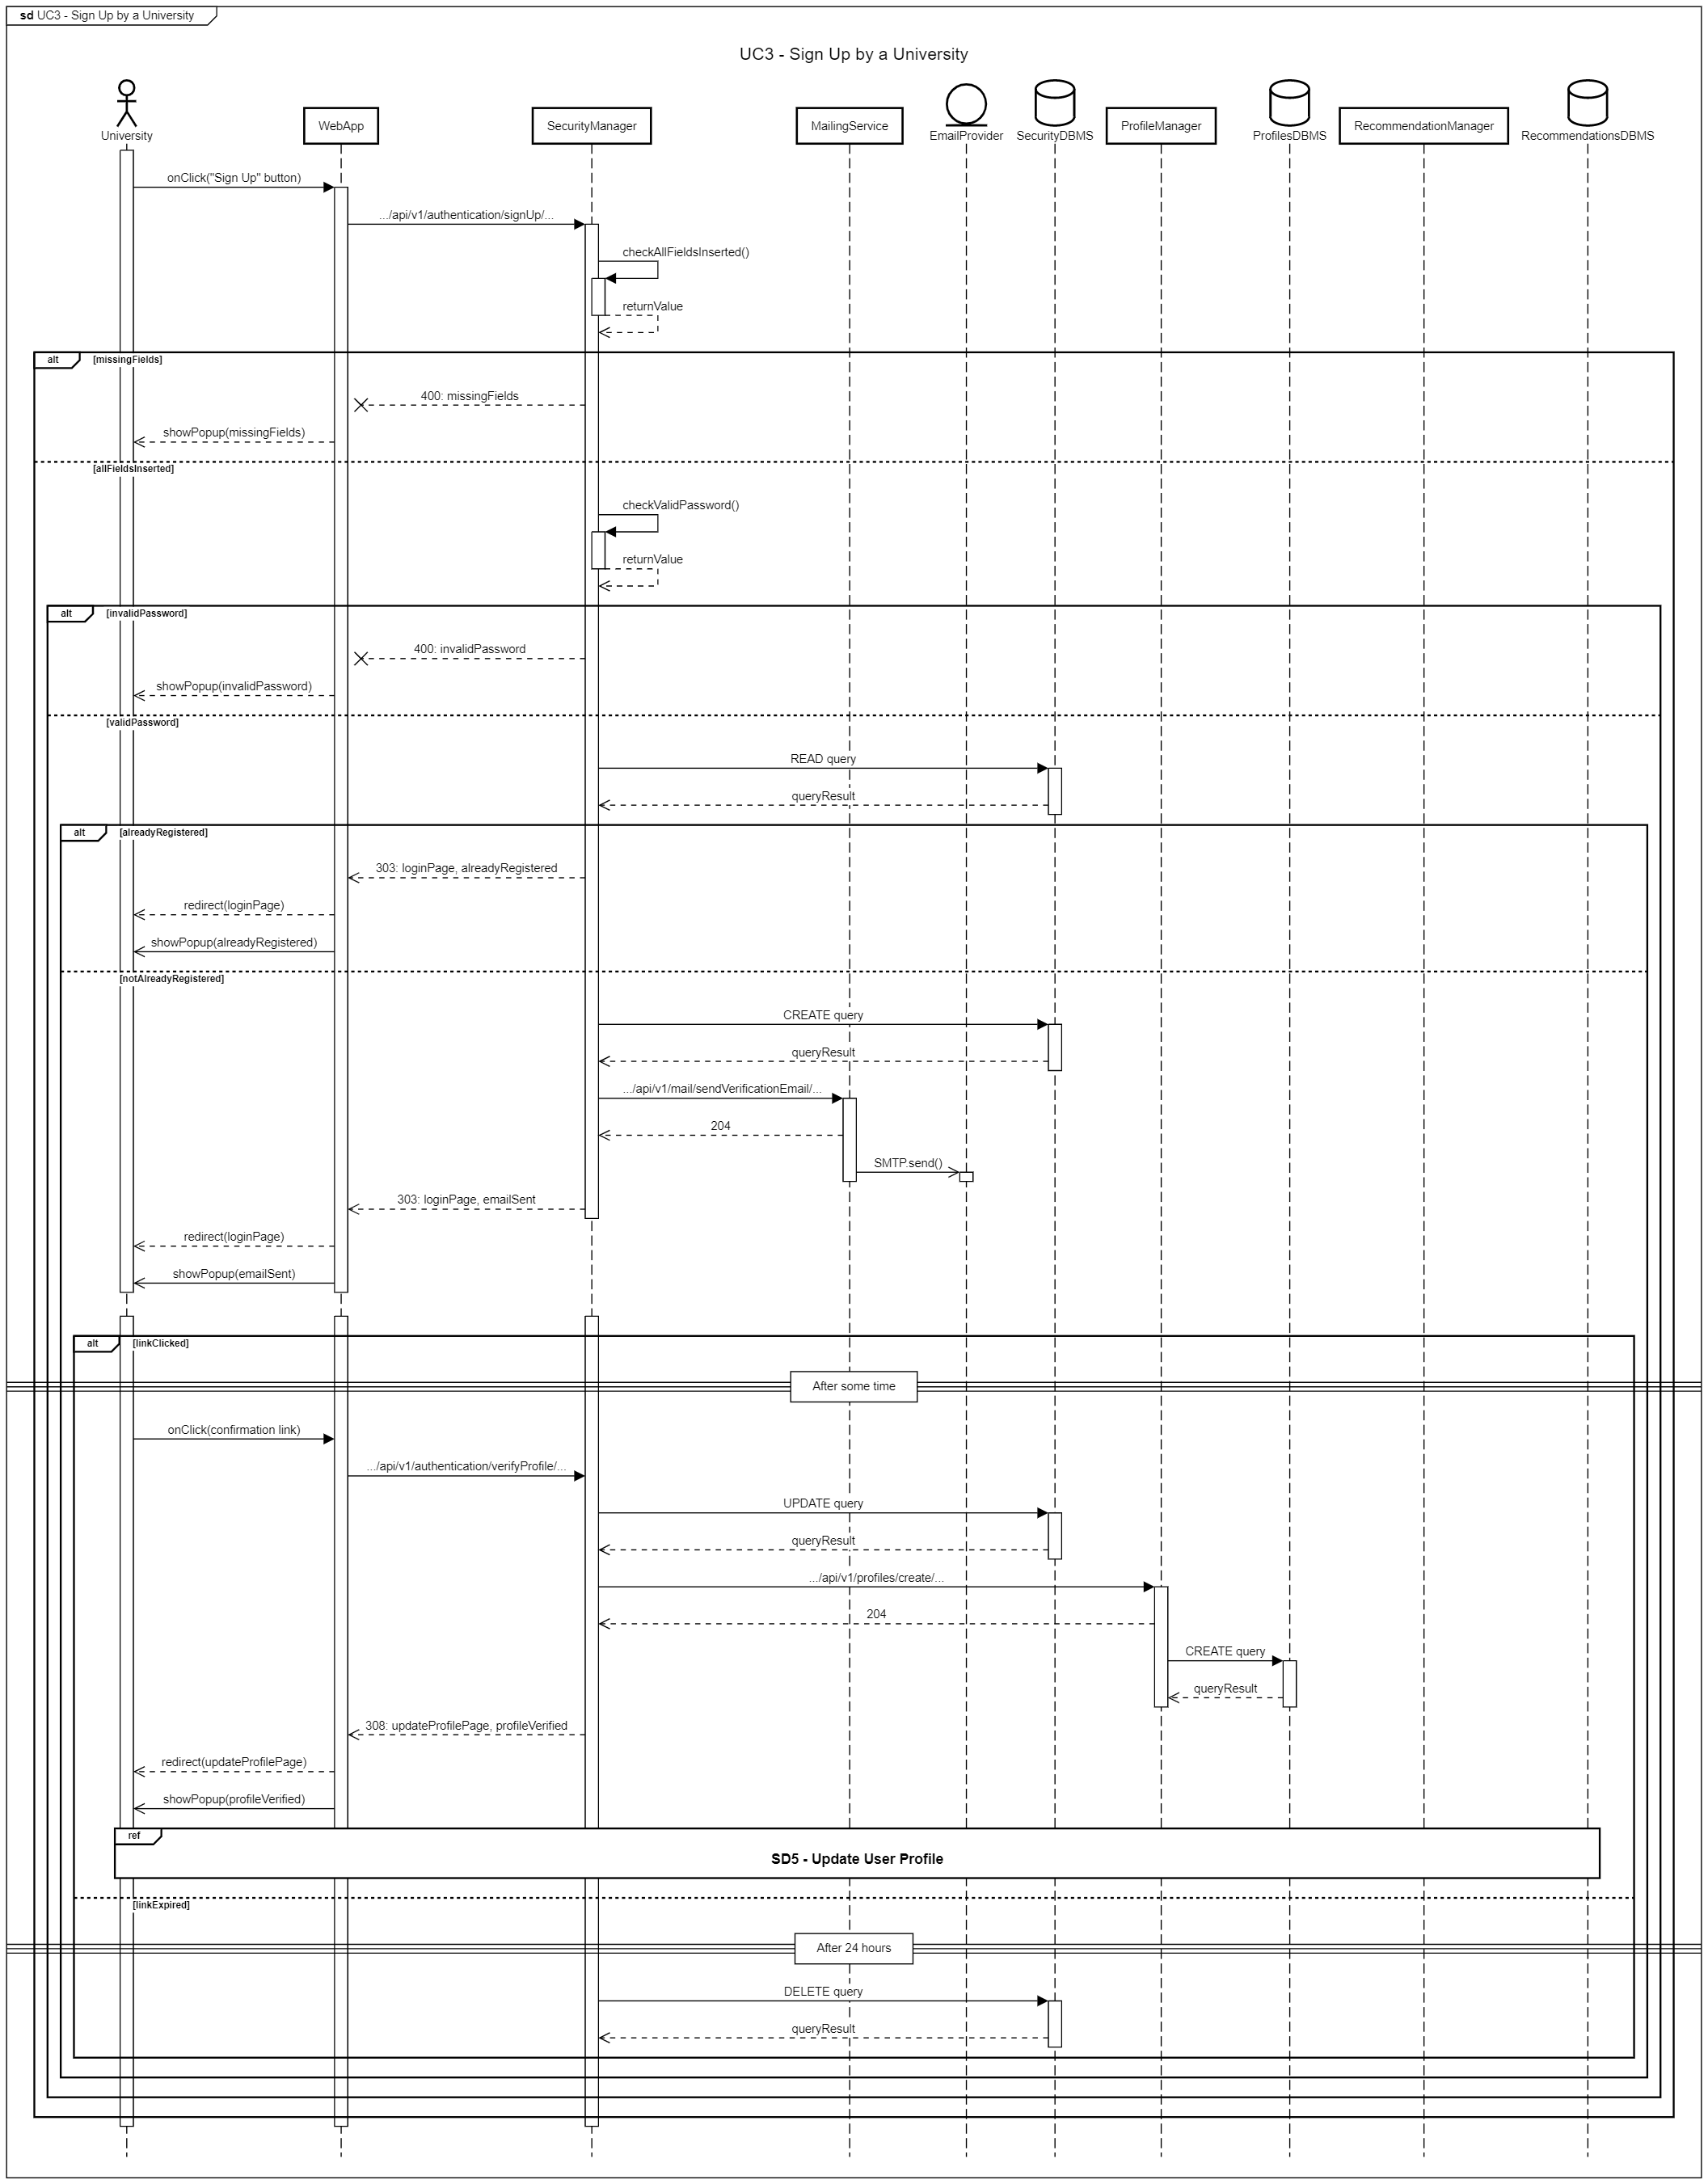
\includegraphics[width=0.9\linewidth]{LaTeXCode/images/SequenceDiagrams/UC3-sequenceDiagram.png}
         \caption{Sign Up by a University}
         \label{fig:signup_university_sd}
     \end{center}
\end{figure}

\subsubsection*{SD\cuc. Log In by a User}
\label{subsubsec:login_user_sd}
The User initiates the process by clicking the "Login" button on the login page, which sends a request to the \texttt{.../api/v1/authentication/login/...} API endpoint. The \texttt{SecurityManager} queries the \texttt{SecurityDBMS} to validate the provided credentials.
If the credentials are correct and the account is verified, the \texttt{SecurityManager} generates an authentication token, which is sent back to the \texttt{WebApp}. Then, the \texttt{SecurityManager} checks whether the User has completed their profile during the signup process. If the profile is incomplete, the User is sent the token and is redirected to the page for updating their profile in order for them to insert the required information; otherwise, they are redirected to the dashboard page with a success status and the token for authentication.

\begin{figure}[H]
    \begin{center}
         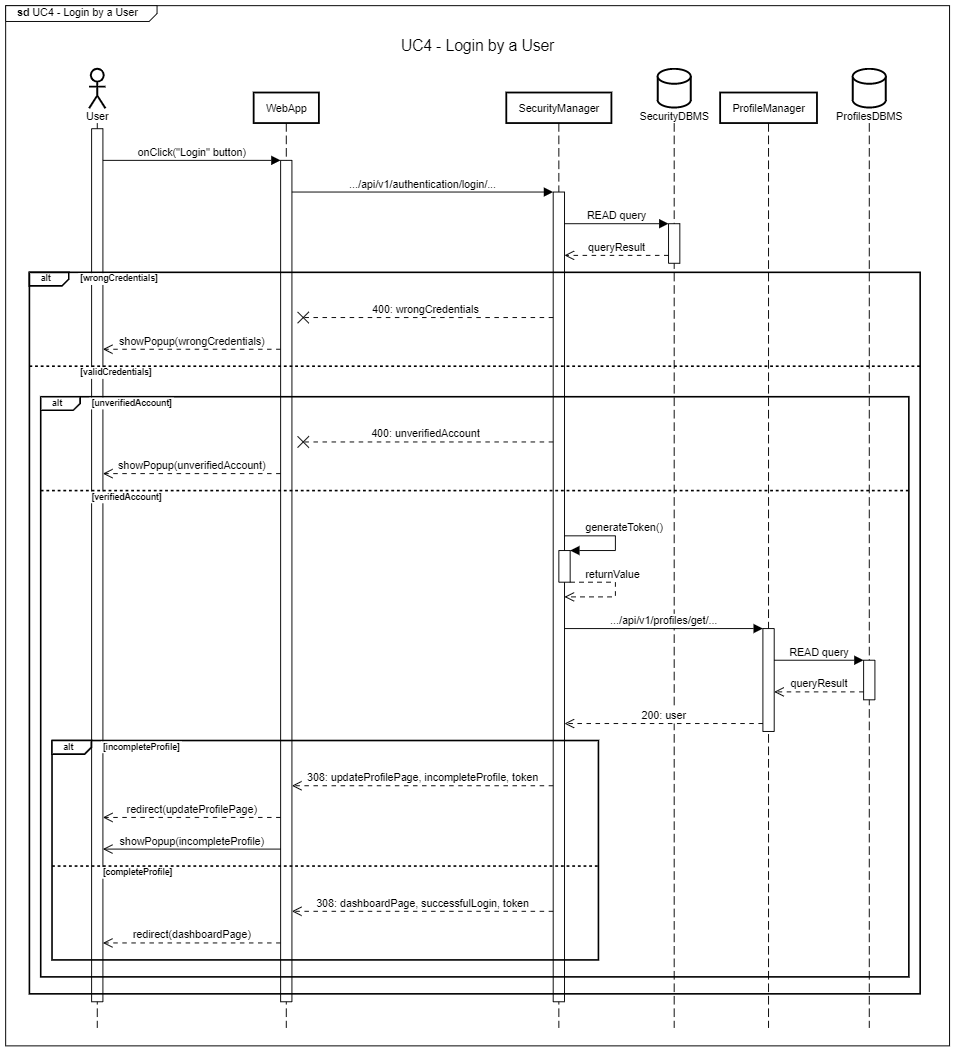
\includegraphics[width=0.8\linewidth]{LaTeXCode/images/SequenceDiagrams/UC4-sequenceDiagram.png}
         \caption{Log In by a User}
         \label{fig:login_user_sd}
     \end{center}
\end{figure}

\subsubsection*{SD\cuc. Update User Profile}
\label{subsubsec:update_profile_sd}
The User initiates the action by clicking the "Apply Changes" button after having inserted updated profile information in the profile update page, triggering a request to the \\ \texttt{.../api/v1/profiles/update/...} API endpoint. The \texttt{ProfileManager} validates the input to ensure all required fields are present.
If the input is valid, the \texttt{ProfileManager} updates the profile data in the \texttt{ProfilesDBMS}, and then notifies the successful update to the WebApp, which shows a popup to the User. The \texttt{ProfileManager} then triggers the \texttt{RecommendationManager} to execute the logic of \hyperref[fig:generate_recommendations_sd]{\protect\uline{SD10 - Generate Recommendations}} for detecting possible new recommendations to be generated.

\begin{figure}[H]
    \begin{center}
         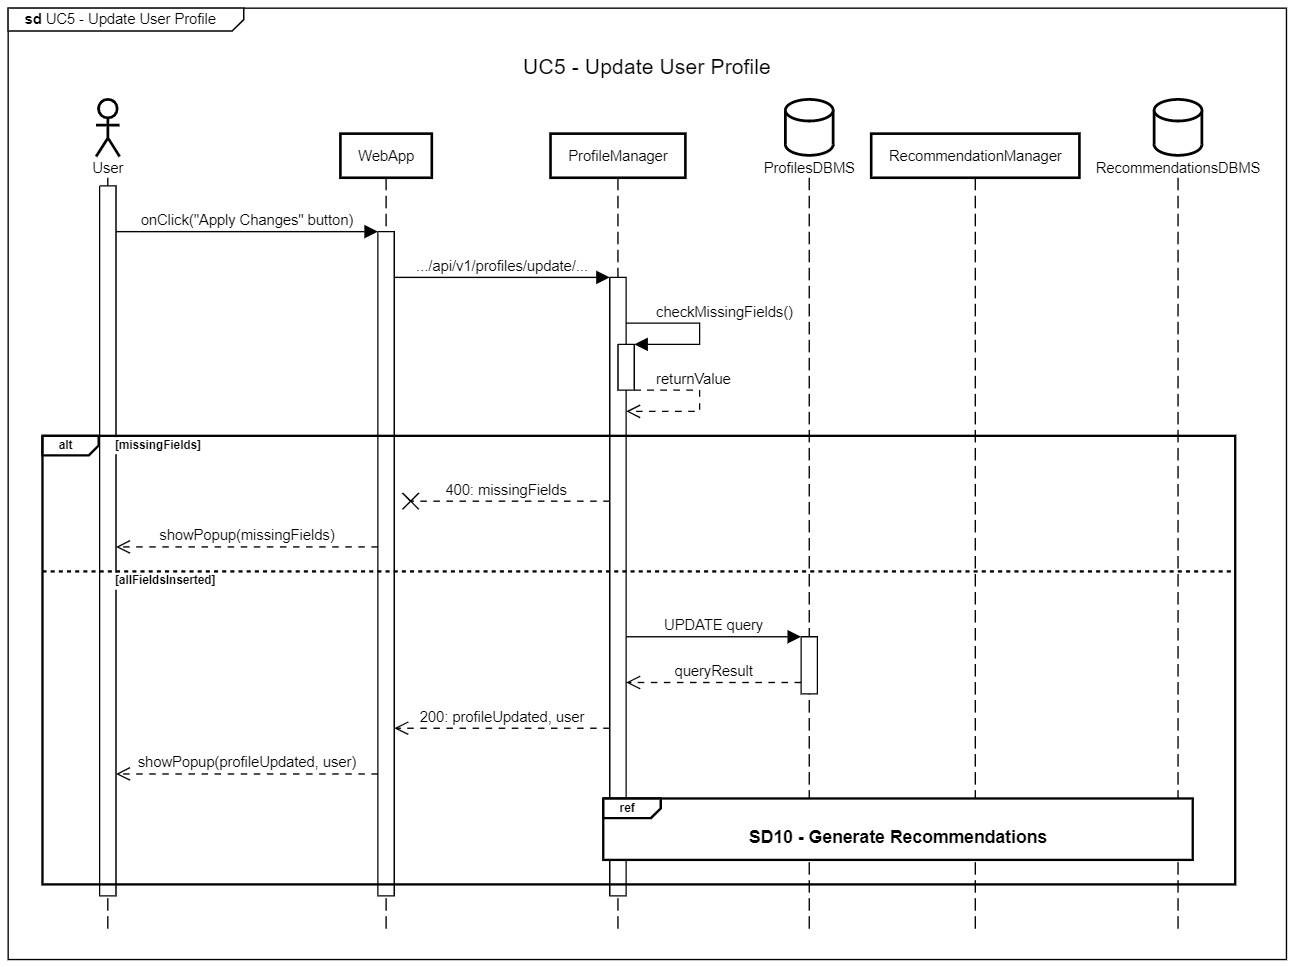
\includegraphics[width=1\linewidth]{LaTeXCode/images/SequenceDiagrams/UC5-sequenceDiagram.png}
         \caption{Update User Profile}
         \label{fig:update_profile_sd}
     \end{center}
\end{figure}

\newpage

\subsubsection*{SD\cuc. Publish an Internship Offer}
\label{subsubsec:publish_offer_sd}
The Company initiates the action by clicking the "Submit" button after having inserted information about the new offer to be posted in the offer creation page, which sends a request to the \texttt{.../api/v1/offers/publish/...} API endpoint. The \texttt{OfferManager} validates the input to ensure all required fields are completed.
If all fields are provided and all the information is compliant the \texttt{OfferManager} creates a new entry in the \texttt{InternshipsDBMS}.
Once the query succeeds, the \texttt{OfferManager} confirms the offer's publication and the Company is notified with a popup indicating that the offer has been successfully published. The component then triggers the \texttt{RecommendationManager} to generate recommendations as part of \hyperref[fig:generate_recommendations_sd]{\protect\uline{SD10 - Generate Recommendations}}.

\begin{figure}[H]
    \begin{center}
         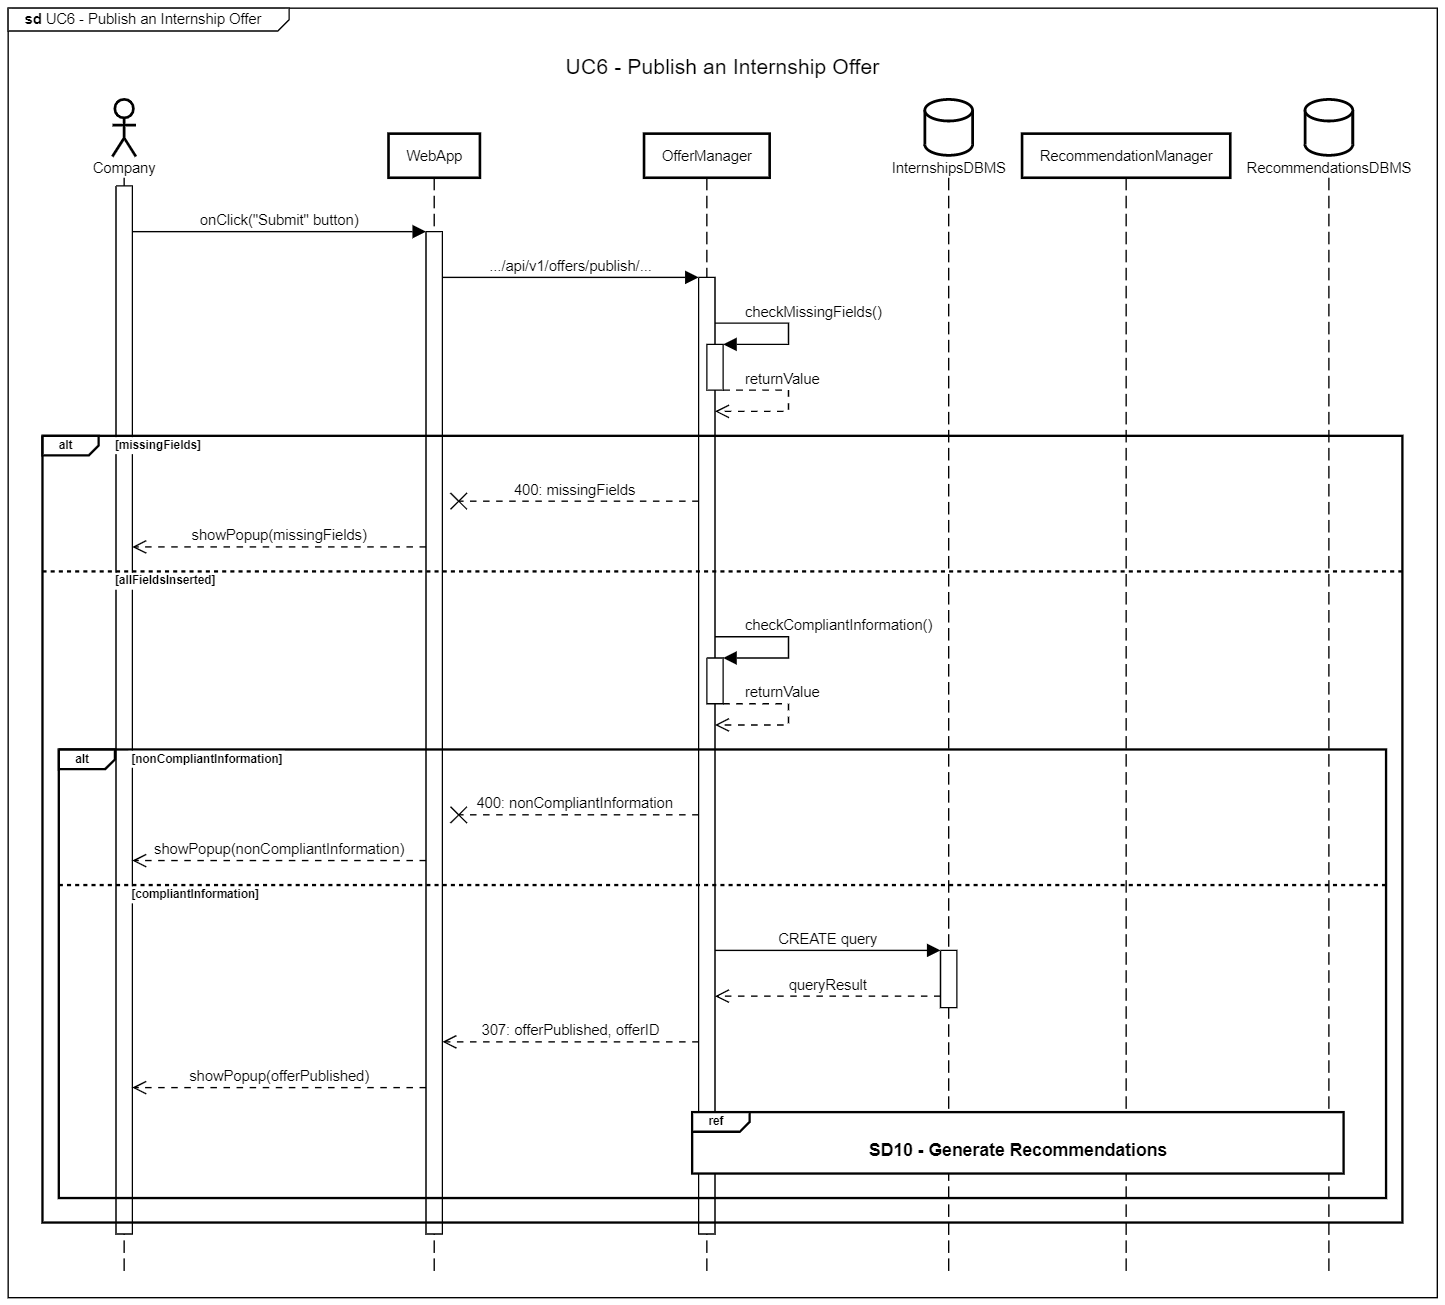
\includegraphics[width=1\linewidth]{LaTeXCode/images/SequenceDiagrams/UC6-sequenceDiagram.png}
         \caption{Publish an Internship Offer}
         \label{fig:publish_offer_sd}
     \end{center}
\end{figure}

\subsubsection*{SD\cuc. Update Internship Offer}
\label{subsubsec:update_internship_offer_sd}
The Company initiates the action either by confirming the withdrawal or by applying changes to one of its offers on the page dedicated to that specific offer. For the withdrawal, the \\ \texttt{.../api/v1/offers/withdraw/...} API endpoint is the one where the request is sent. The \texttt{OfferManager} retrieves related "Unhandled" recommendations by interacting with the \\ \texttt{RecommendationManager}, which in turn queries the \texttt{RecommendationsDBMS}, and subsequently asks the exposed API to discard them. Then the \texttt{OfferManager} doesn't DELETE the offer, but only performs an UPDATE query for its status in the \texttt{InternshipsDBMS}, so that its data doesn't get lost. Finally, the component redirects the Company to the dashboard with a success alert.
When updating offer information, the request is instead forwarded to the \texttt{.../api/v1/offers/update/...} API endpoint. The \texttt{OfferManager} validates the input for missing fields and compliance. If valid, the updated information is stored in the \texttt{InternshipsDBMS}, and the system notifies the Company of the successful update, in the end triggering the \texttt{RecommendationManager} to generate new recommendations as defined in \hyperref[fig:generate_recommendations_sd]{\protect\uline{SD10 - Generate Recommendations}}.

\newpage

\begin{figure}[H]
    \begin{center}
         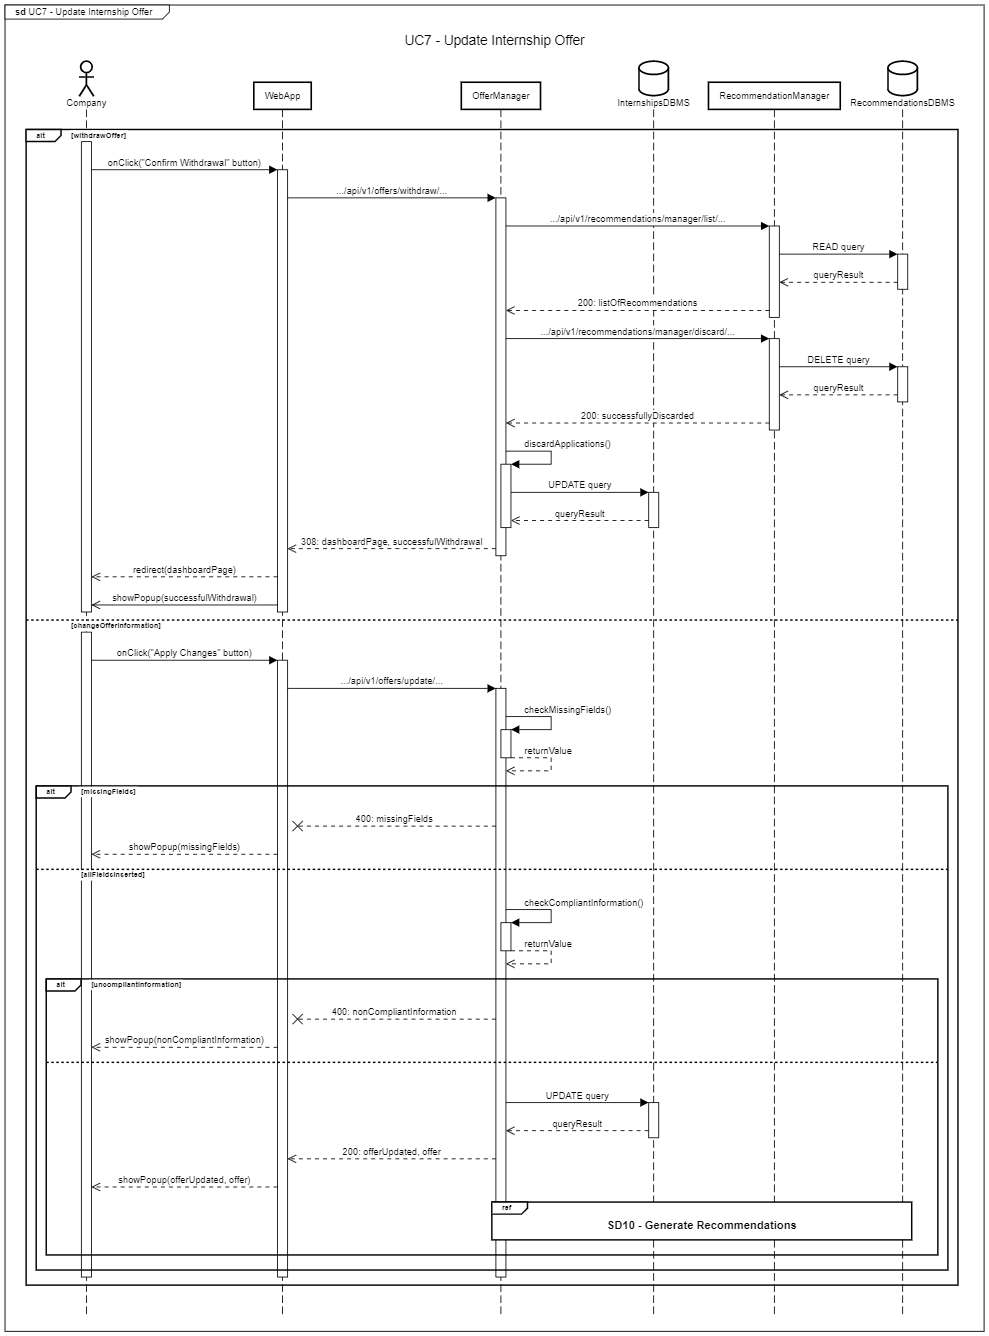
\includegraphics[width=1\linewidth]{LaTeXCode/images/SequenceDiagrams/UC7-sequenceDiagram.png}
         \caption{Update Internship Offer}
         \label{fig:update_internship_offer_sd}
     \end{center}
\end{figure}

\subsubsection*{SD\cuc. Search Internship Offers}
\label{subsubsec:search_offer_sd}
The Student initiates the action by clicking the "Submit" button on the dashboard page after having inserted the filter criteria, triggering a request to the \texttt{.../api/v1/offers/search/...} API endpoint. The \texttt{OfferManager} processes the request and queries the \texttt{InternshipsDBMS} using a READ operation to fetch the relevant internship offers which match the search query criteria.
The \texttt{OfferManager} returns the query results to the \texttt{WebApp}, which displays the results to the Student. If no results are found, the system shows a custom message of the list of internships instead.

\begin{figure}[H]
    \begin{center}
         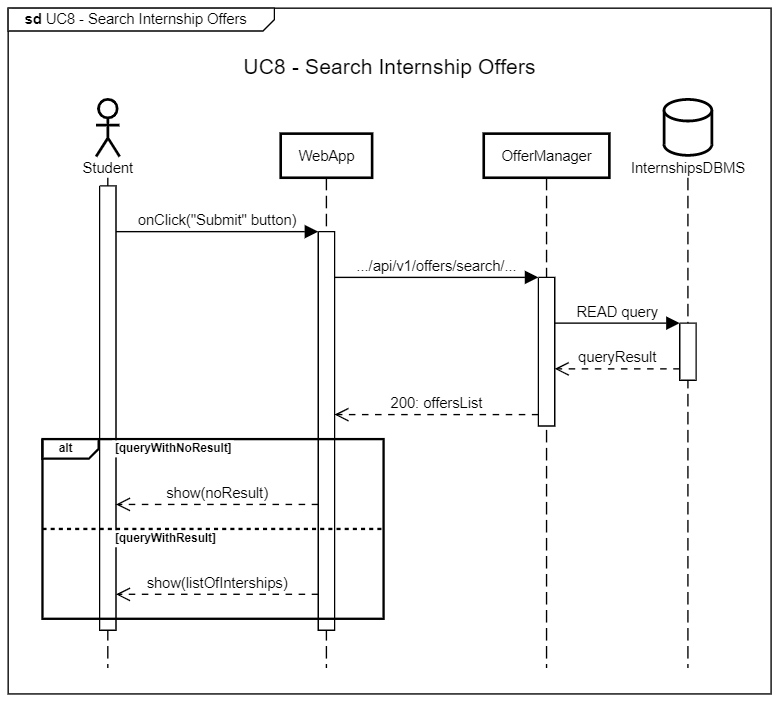
\includegraphics[width=1\linewidth]{LaTeXCode/images/SequenceDiagrams/UC8-sequenceDiagram.png}
         \caption{Search Internship Offers}
         \label{fig:search_offer_sd}
     \end{center}
\end{figure}

\subsubsection*{SD\cuc. Apply to an Internship Offer}
\label{subsubsec:apply_to_internships_sd}
The Student submits an application for an internship offer by clicking the "Apply" button on an offer's page, invoking the \texttt{.../api/v1/offers/apply/...} API endpoint. The \texttt{OfferManager} first verifies the deadline through the \texttt{InternshipsDBMS}: if the deadline has expired, an error is shown to the Student; otherwise, the \texttt{OfferManager} calls the \texttt{RecommendationManager}, which interacts with the \texttt{RecommendationsDBMS} to accept the recommendations of the applicating Student about that offer and to discard the recommendations of the offering Company about that Student for that Offer, as expected by the functional requirements. Finally, the application is recorded in the \texttt{InternshipsDBMS}, and the Student is notified of the successful submission.

\begin{figure}[H]
    \begin{center}
         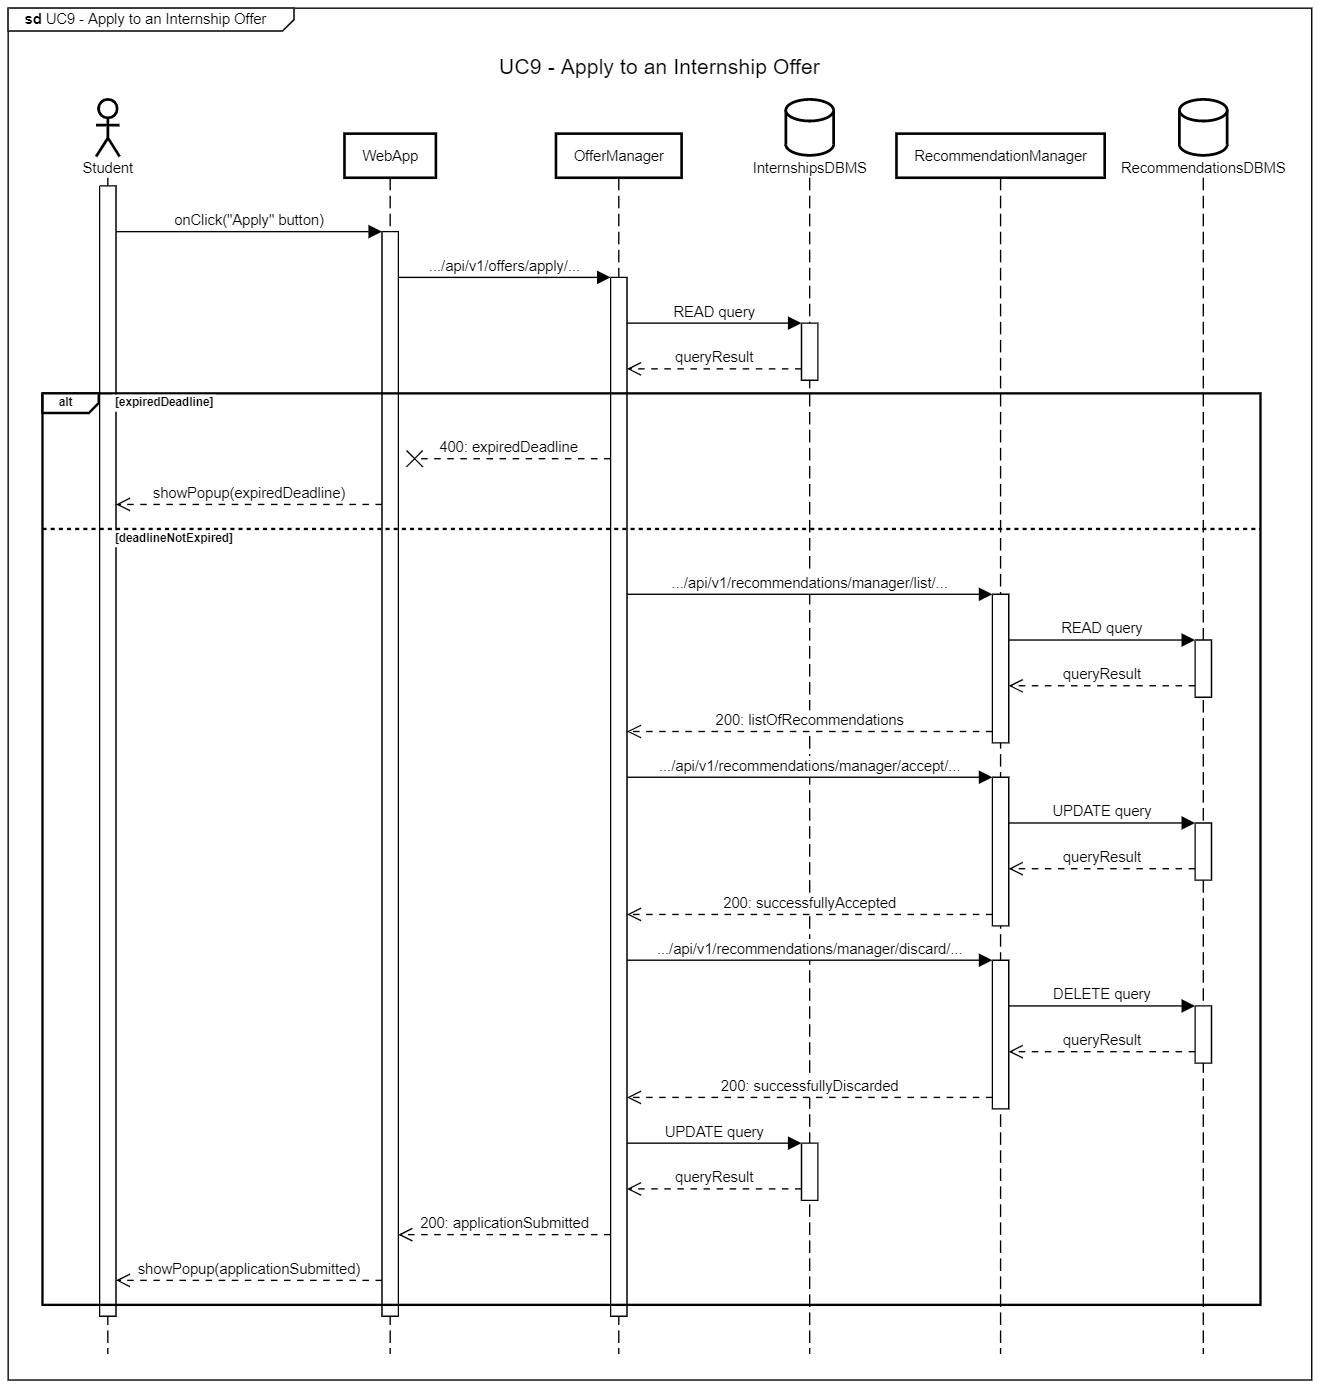
\includegraphics[width=0.9\linewidth]{LaTeXCode/images/SequenceDiagrams/UC9-sequenceDiagram.png}
         \caption{Apply to an Internship Offer}
         \label{fig:apply_to_internships_sd}
     \end{center}
\end{figure}

\subsubsection*{SD\cuc. Generate Recommendations}
\label{subsubsec:generate_recommendations_sd}
The process can be triggered either by a profile update through the \texttt{ProfileManager} or an internship offer update via the \texttt{OfferManager}, both invoking the \\ \texttt{.../api/v1/recommendations/generator/generate/...} API endpoint.
Upon invocation, the \texttt{RecommendationManager} queries the \texttt{RecommendationDBMS} to retrieve relevant data for generating new recommendations. Once the query is completed and the data is processed, the new recommendations are pushed into the \texttt{RecommendationDBMS}.

\begin{figure}[H]
    \begin{center}
         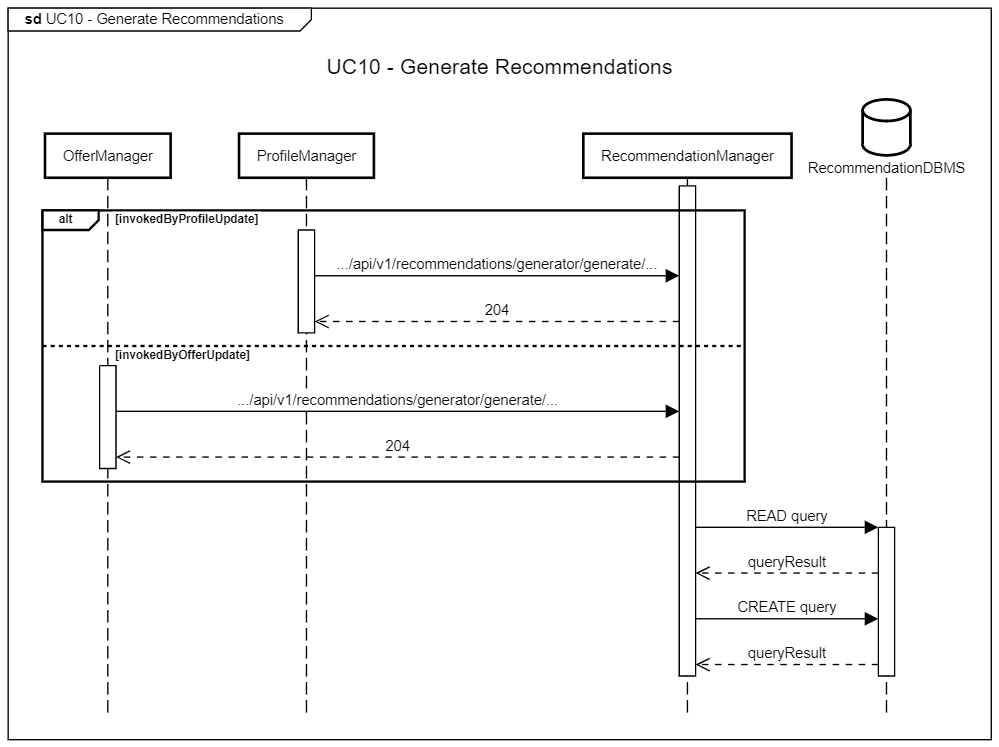
\includegraphics[width=1\linewidth]{LaTeXCode/images/SequenceDiagrams/UC10-sequenceDiagram.png}
         \caption{Generate Recommendations}
         \label{fig:generate_recommendations_sd}
     \end{center}
\end{figure}

\newpage

\subsubsection*{SD\cuc. Manage Internship Recommendations}
\label{subsubsec:manage_internship_recommendations_sd}
For each of their "Unhandled" recommendations, the Student can either accept it, reject it, or postpone the decision. Whether the Student clicks the "Accept" or the "Reject" button on a recommendation's widget, triggering the corresponding \texttt{.../api/v1/recommendations/manager/...} API endpoint of the \texttt{RecommendationManager}, the status of the recommendation in the \\ \texttt{RecommendationsDBMS} is updated accordingly. In case of acceptance, an application for the offer from the Student is also generated, as discussed in the functional requirements, by invoking \hyperref[fig:apply_to_internships_sd]{\protect\uline{SD9 - Apply to an Internship Offer}}. A confirmation popup for the success of the operation is finally displayed to the Student. Recommendations postponed (for which no action is taken) remain unaltered.

\begin{figure}[H]
    \begin{center}
         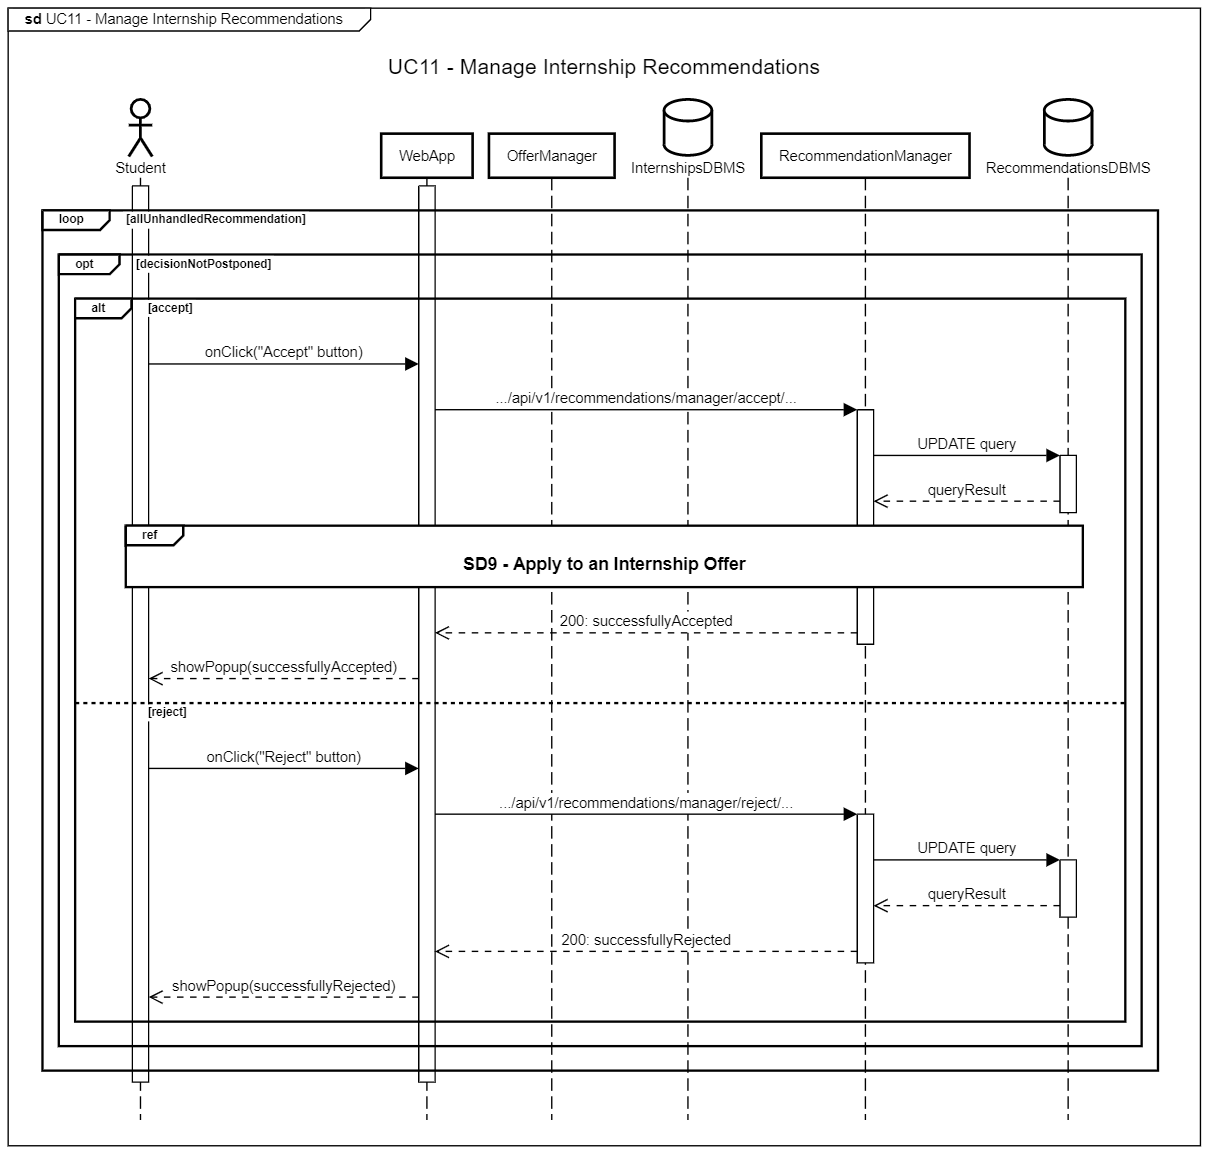
\includegraphics[width=0.9\linewidth]{LaTeXCode/images/SequenceDiagrams/UC11-sequenceDiagram.png}
         \caption{Manage Internship Recommendations}
         \label{fig:manage_internship_recommendations_sd}
     \end{center}
\end{figure}

\subsubsection*{SD\cuc. Manage Students Recommendations}
\label{subsubsec:manage_students_recommendations_sd}
Similar to the previous one, the following Sequence Diagram describes the process of recommendations management by a Company. The only difference is that, instead of generating an offer application, when accepting a recommendation a new one is generated for the corresponding Student if they don't already have one.

\begin{figure}[H]
    \begin{center}
         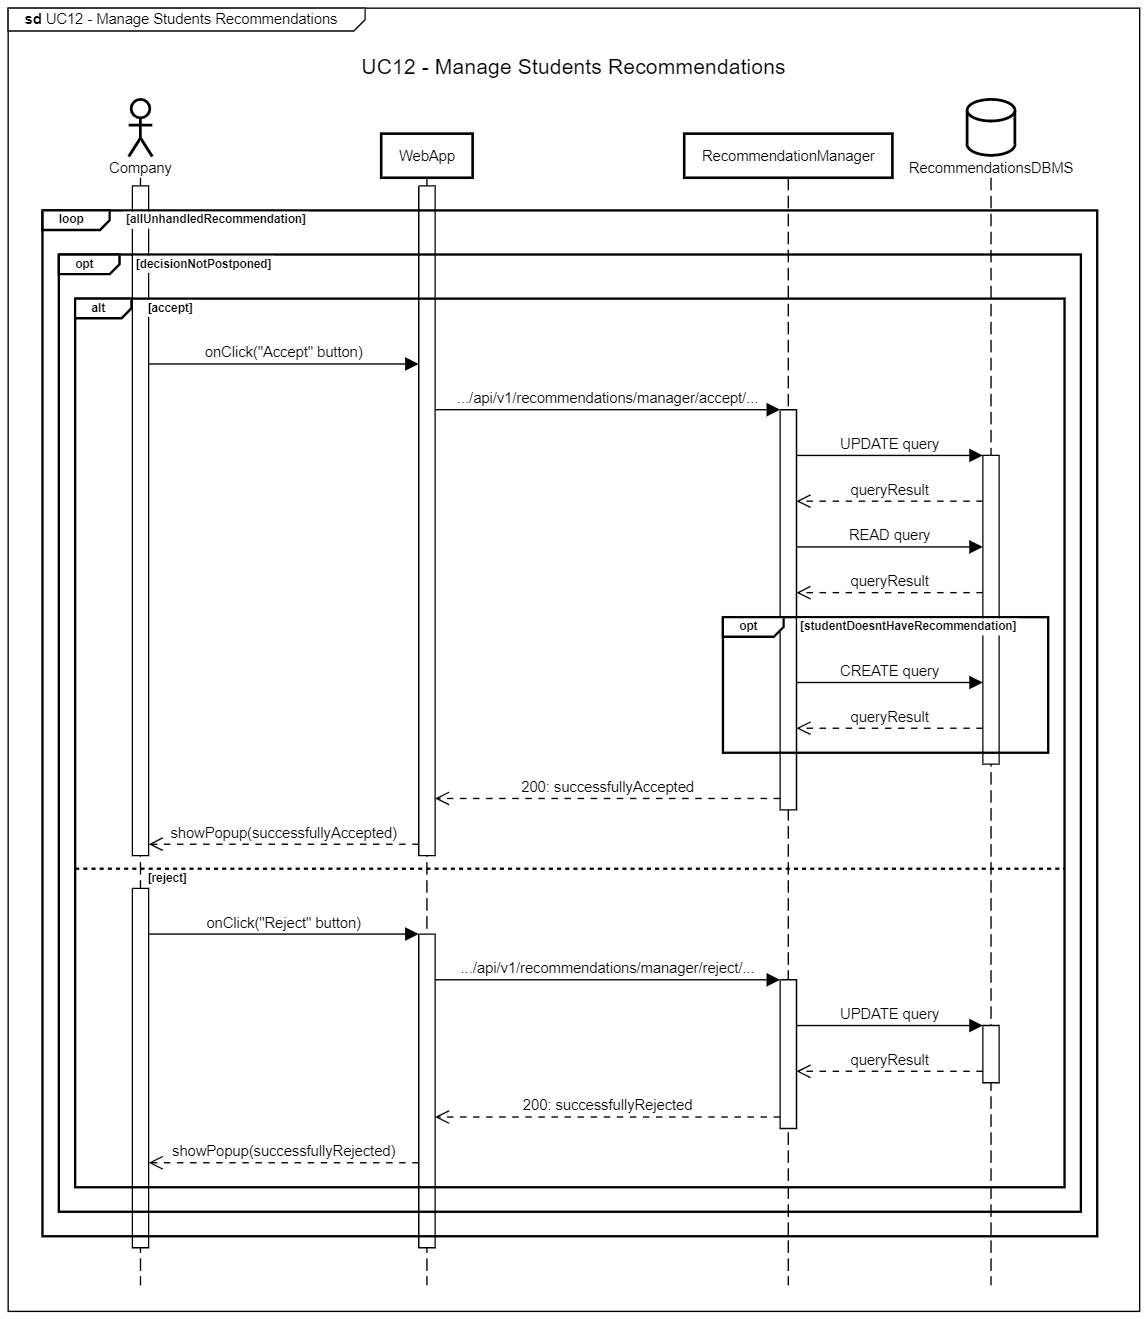
\includegraphics[width=0.9\linewidth]{LaTeXCode/images/SequenceDiagrams/UC12-sequenceDiagram.png}
         \caption{Manage Students Recommendations}
         \label{fig:manage_students_recommendations_sd}
     \end{center}
\end{figure}

\subsubsection*{SD\cuc. Manage an Interview}
\label{subsubsec:manage_interview_sd}
This Sequence Diagram illustrates the process of scheduling, conducting, and evaluating an interview between a Company and a Student.
\begin{enumerate}
    \item The Company first clicks the "Send Invitation" button on its dashboard, sending an interview invitation through the \texttt{.../api/v1/interviews/sendInvitation/...} API endpoint, managed by the \texttt{InterviewManager}, which creates an entry in the \texttt{InternshipsDBMS} for the invitation. The Student may accept or decline the invitation by clicking the corresponding buttons, which invoke the respective \texttt{.../api/v1/internships/...} API endpoint:
    \begin{itemize}
        \item If accepted, the \texttt{InterviewManager} updates the status in the \texttt{InternshipsDBMS}, and the Student is notified.
        \item If declined, the \texttt{InternshipsDBMS} is updated accordingly, and the Company may decide to try to reschedule it based on the motivation provided by the Student.
    \end{itemize}
    This phase loops until either the Student accepts one invitation, or the Company decides that no agreement can be reached and stops the process.
    
    \item For in-platform interviews only, the Company posts some questions via the "Post Questions" button, which calls the \texttt{.../api/v1/interviews/createQuestions/...} API endpoint, and when the scheduled time comes the Student involved in the interview replies to each question and submits their answer through the "Submit" button of the specific question in its dashboard, which interacts with the system through the \\ \texttt{.../api/v1/interviews/submitAnswer/...} API endpoint. The questions and the answers are recorded in the \texttt{InternshipsDBMS}, and popups are shown to both parties to confirm their submissions.

    \item After the interview, the Company evaluates the candidate by submitting the results through the specific "Evaluate" button, calling \texttt{.../api/v1/interviews/evaluate/...} API endpoint. The result and eventual feedback are stored in the \texttt{InternshipsDBMS} by updating the interview status, and the Company is notified of the successful evaluation.
\end{enumerate}

\newpage

\begin{figure}[H]
    \begin{center}
         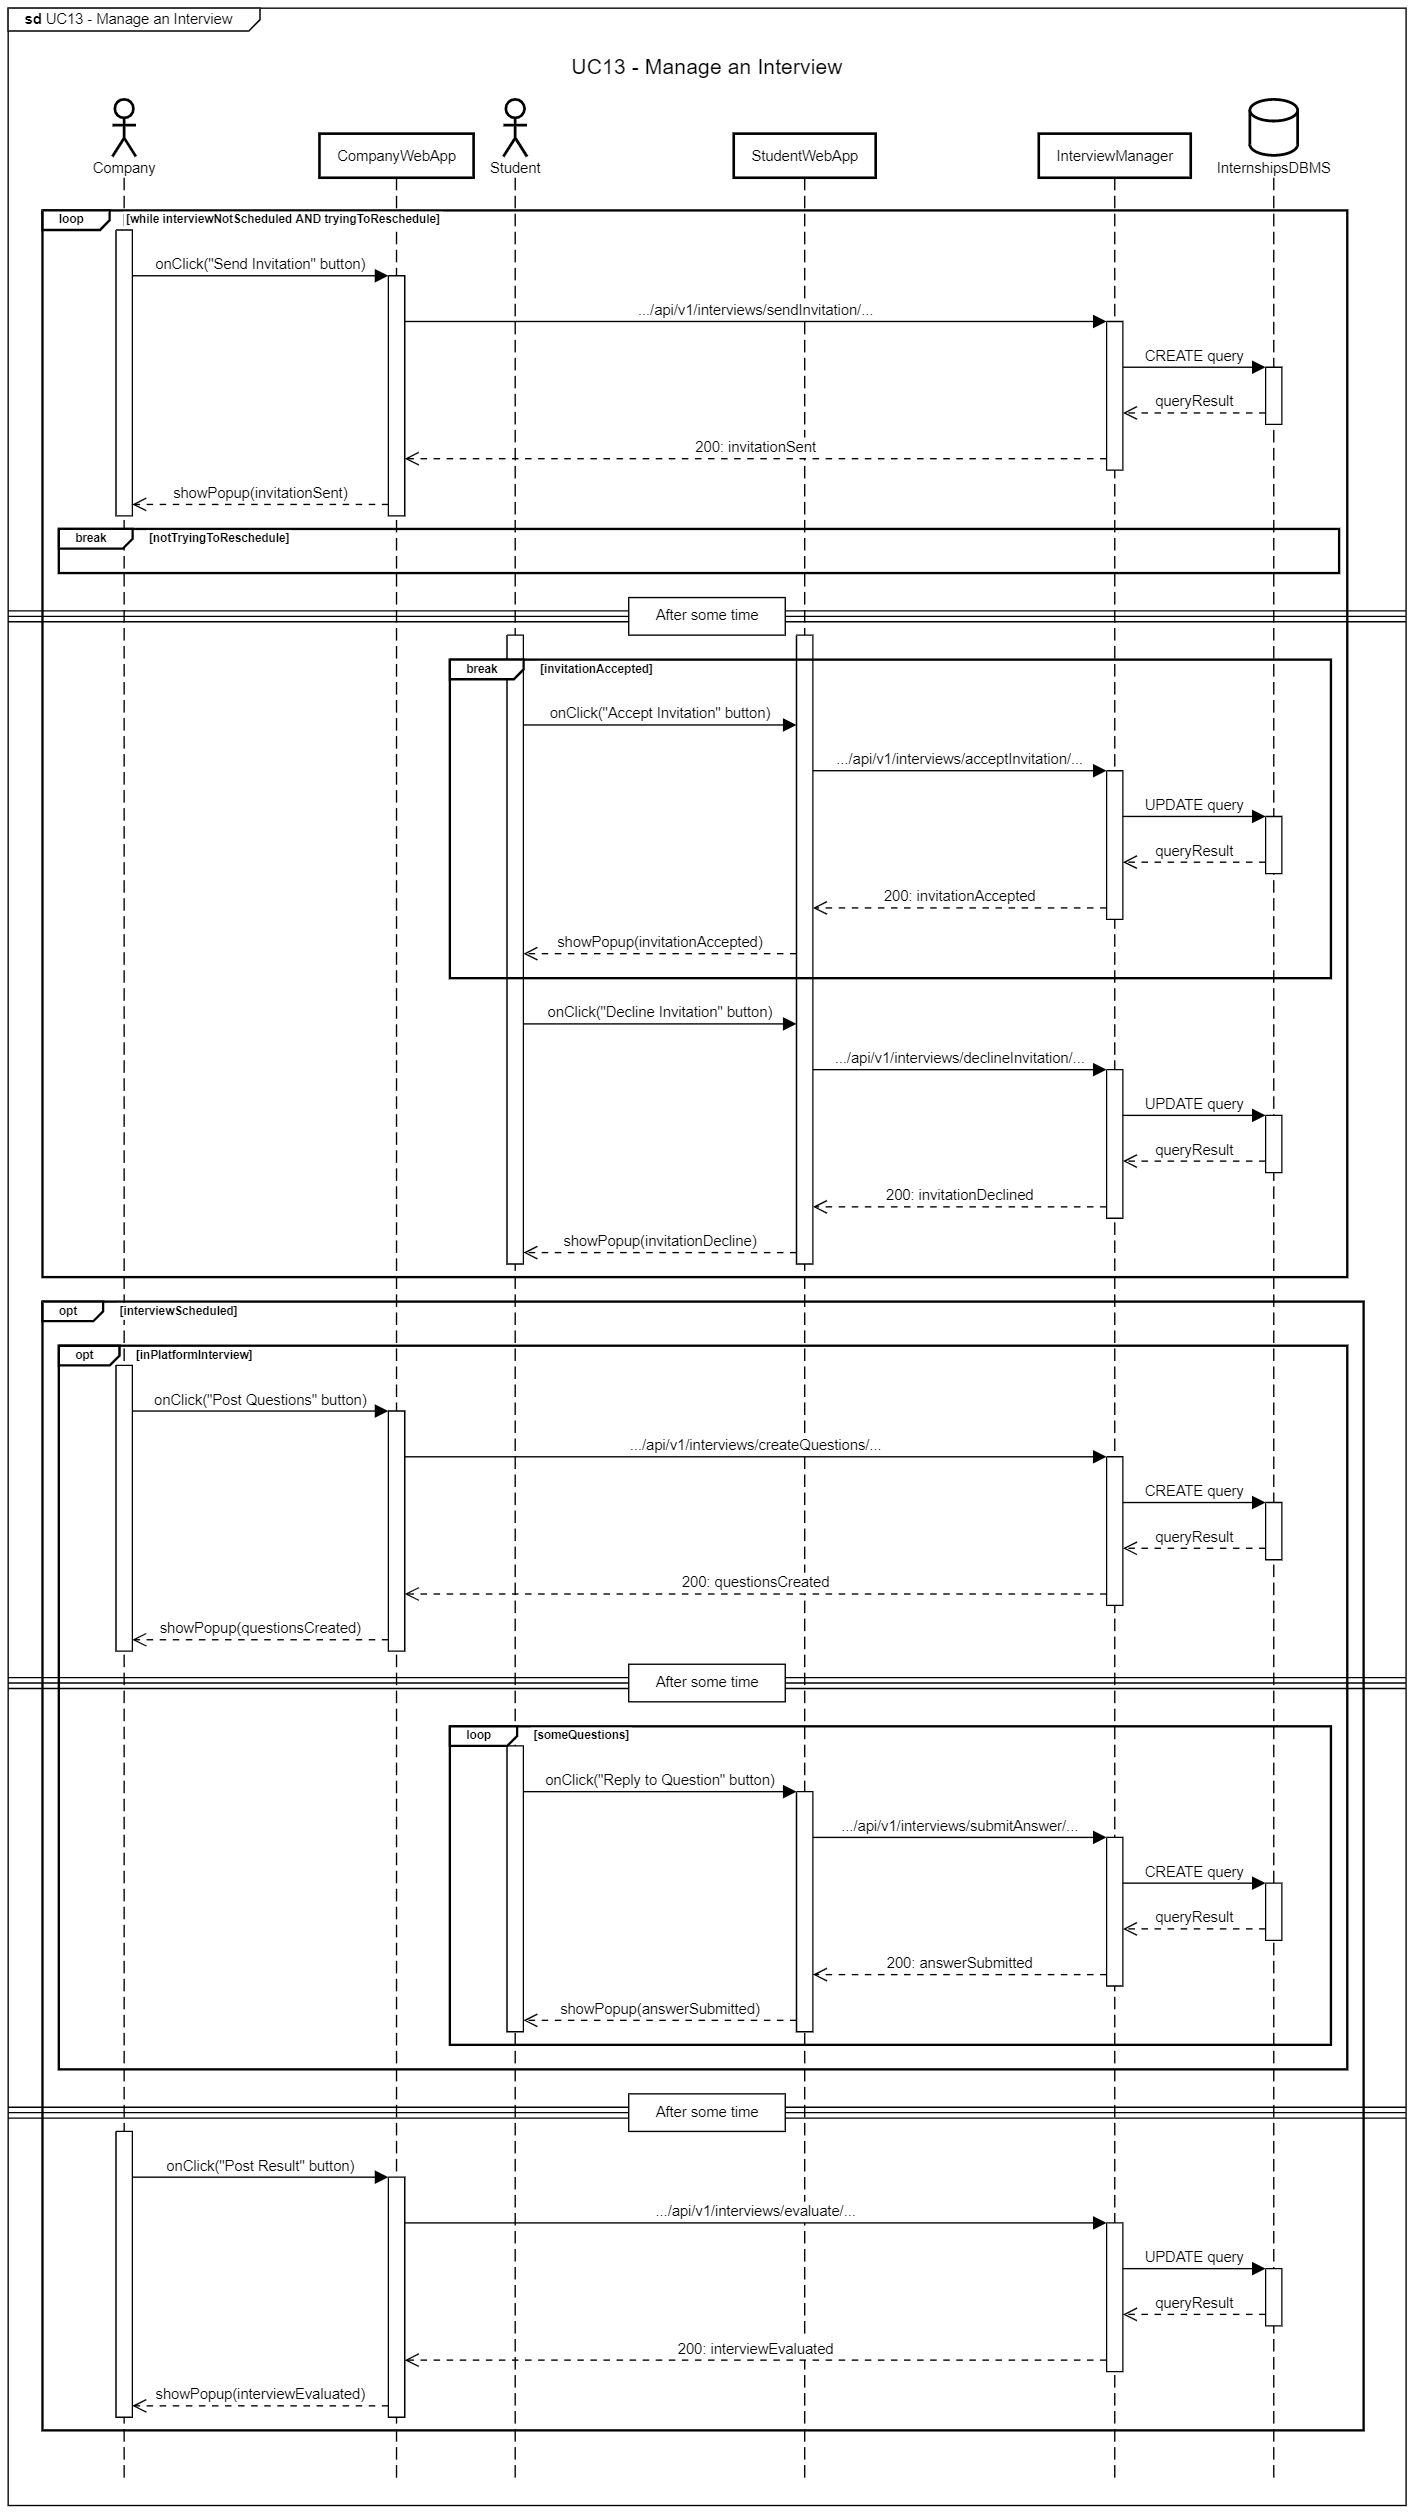
\includegraphics[width=0.8\linewidth]{LaTeXCode/images/SequenceDiagrams/UC13-sequenceDiagram.png}
         \caption{Manage an Interview}
         \label{fig:manage_interview_sd}
     \end{center}
\end{figure}

\subsubsection*{SD\cuc. Provide Information for an ongoing Internship}
\label{subsubsec:provide_information_ongoing_sd}
The Party initiates the process by clicking the "Post Information"  on an ongoing internship's page, which triggers a request to the \texttt{.../api/v1/internships/addInformation/...} API endpoint handled by the \texttt{IMFManager}. The \texttt{IMFManager} adds the new internship data in the \texttt{InternshipsDBMS}. Once the operation is successfully completed, the \texttt{WebApp} receives a confirmation and displays a popup notifying the Party of the successful submission.

\begin{figure}[H]
    \begin{center}
         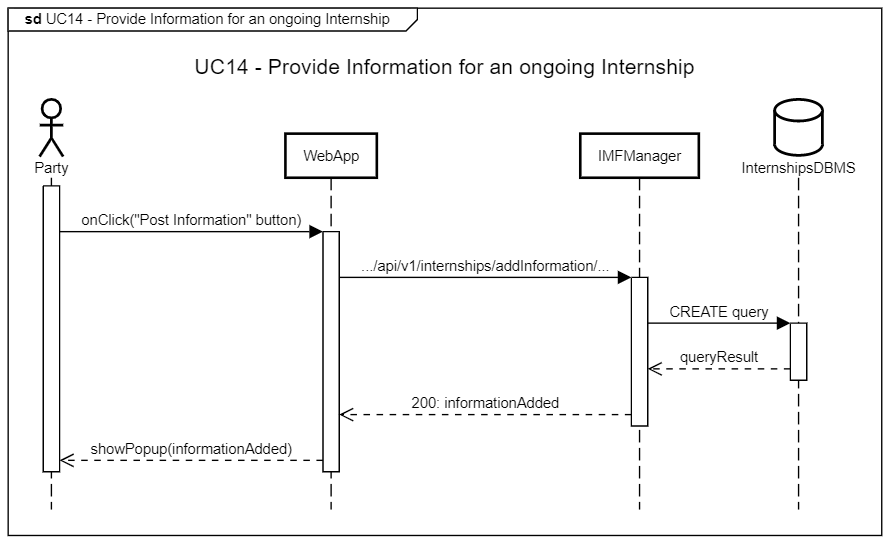
\includegraphics[width=1\linewidth]{LaTeXCode/images/SequenceDiagrams/UC14-sequenceDiagram.png}
         \caption{Provide Information for an ongoing Internship}
         \label{fig:provide_information_ongoing_sd}
     \end{center}
\end{figure}

\newpage

\subsubsection*{SD\cuc. Monitor an ongoing Internship}
\label{subsubsec:monitor_internship_sd}
The Party selects an internship widget, sending a request to the \texttt{.../api/v1/internships/get/...} API endpoint handled by the \texttt{IMFManager}. The \texttt{IMFManager} retrieves the internship details from the \texttt{InternshipsDBMS}. Upon successfully fetching the data, the \texttt{WebApp} displays the internship details to the Party.
Additionally, in the visualized section the Party can also optionally provide new information about the internship if they need to, referring to the process detailed in \hyperref[fig:provide_information_ongoing_sd]{\protect\uline{SD14 - Provide Information for an ongoing Internship}}.

\begin{figure}[H]
    \begin{center}
         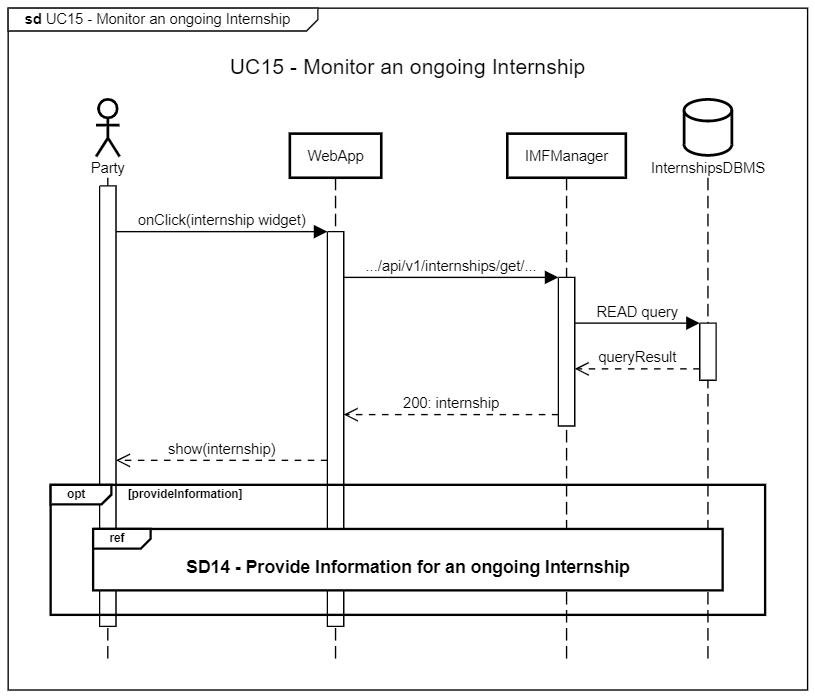
\includegraphics[width=1\linewidth]{LaTeXCode/images/SequenceDiagrams/UC15-sequenceDiagram.png}
         \caption{Monitor an ongoing Internship}
         \label{fig:monitor_internship_sd}
     \end{center}
\end{figure}

\newpage

\subsubsection*{SD\cuc. Report Problems during an Internship}
\label{subsubsec:report_problems_sd}
The Party initiates the process by clicking the "Report" button on an ongoing internship's page, triggering a request to the \texttt{.../api/v1/internships/reportProblem/...} API endpoint exposed by the \texttt{IMFManager}, which checks the submitted fields for completeness. If all fields are provided, the \texttt{IMFManager} records the problem in the \texttt{InternshipsDBMS} creating a new entry. Once the problem is successfully reported, the \texttt{WebApp} notifies the Party with the appropriate confirmation popup.

\begin{figure}[H]
    \begin{center}
         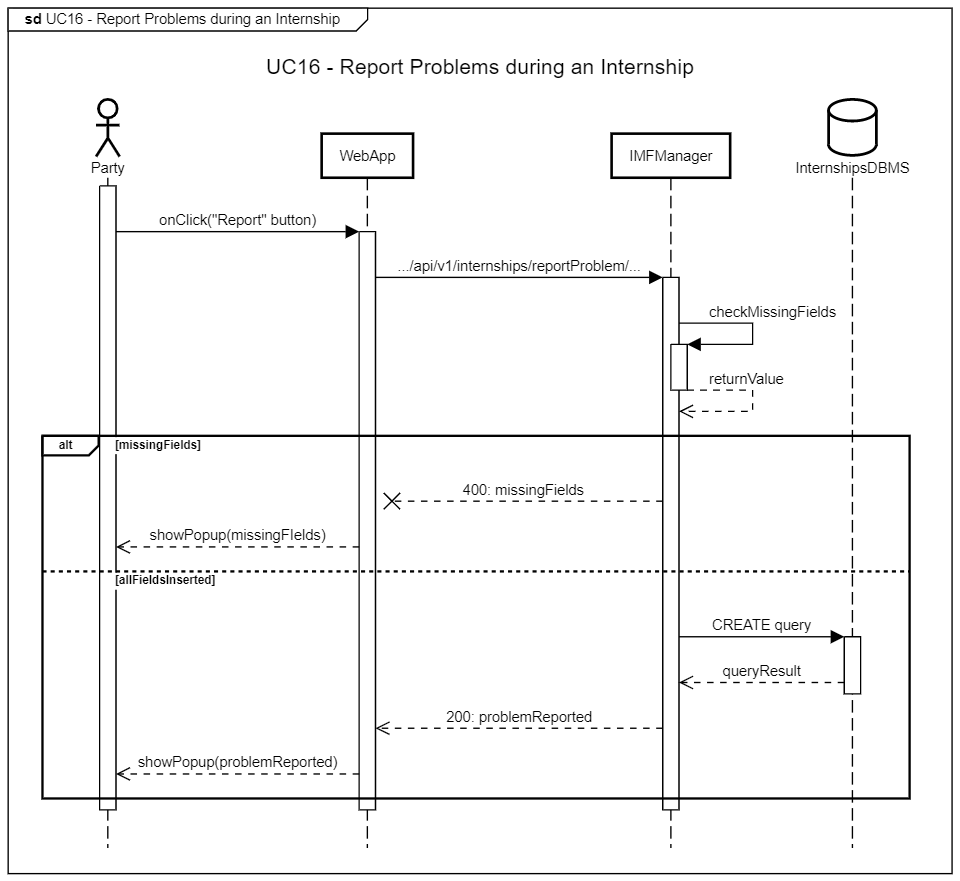
\includegraphics[width=1\linewidth]{LaTeXCode/images/SequenceDiagrams/UC16-sequenceDiagram.png}
         \caption{Report Problems during an Internship}
         \label{fig:report_problems_sd}
     \end{center}
\end{figure}

\newpage

\subsubsection*{SD\cuc. Handle Problems during an Internship}
\label{subsubsec:handle_problems_sd}
The University initiates the process by clicking one of the "Mark as In Progress", "Mark as Solved" or "Hide" buttons on a problem's widget in its dashboard page, triggering a request to the \texttt{.../api/v1/internships/handleProblem/...} API endpoint, managed by the \texttt{IMFManager}. The \texttt{IMFManager} updates the problem's status in the \texttt{InternshipsDBMS} according to the button clicked by the University. Upon successful completion, the \texttt{WebApp} receives confirmation and notifies the University with a popup indicating that the problem has been correctly marked as solved.

\begin{figure}[H]
    \begin{center}
         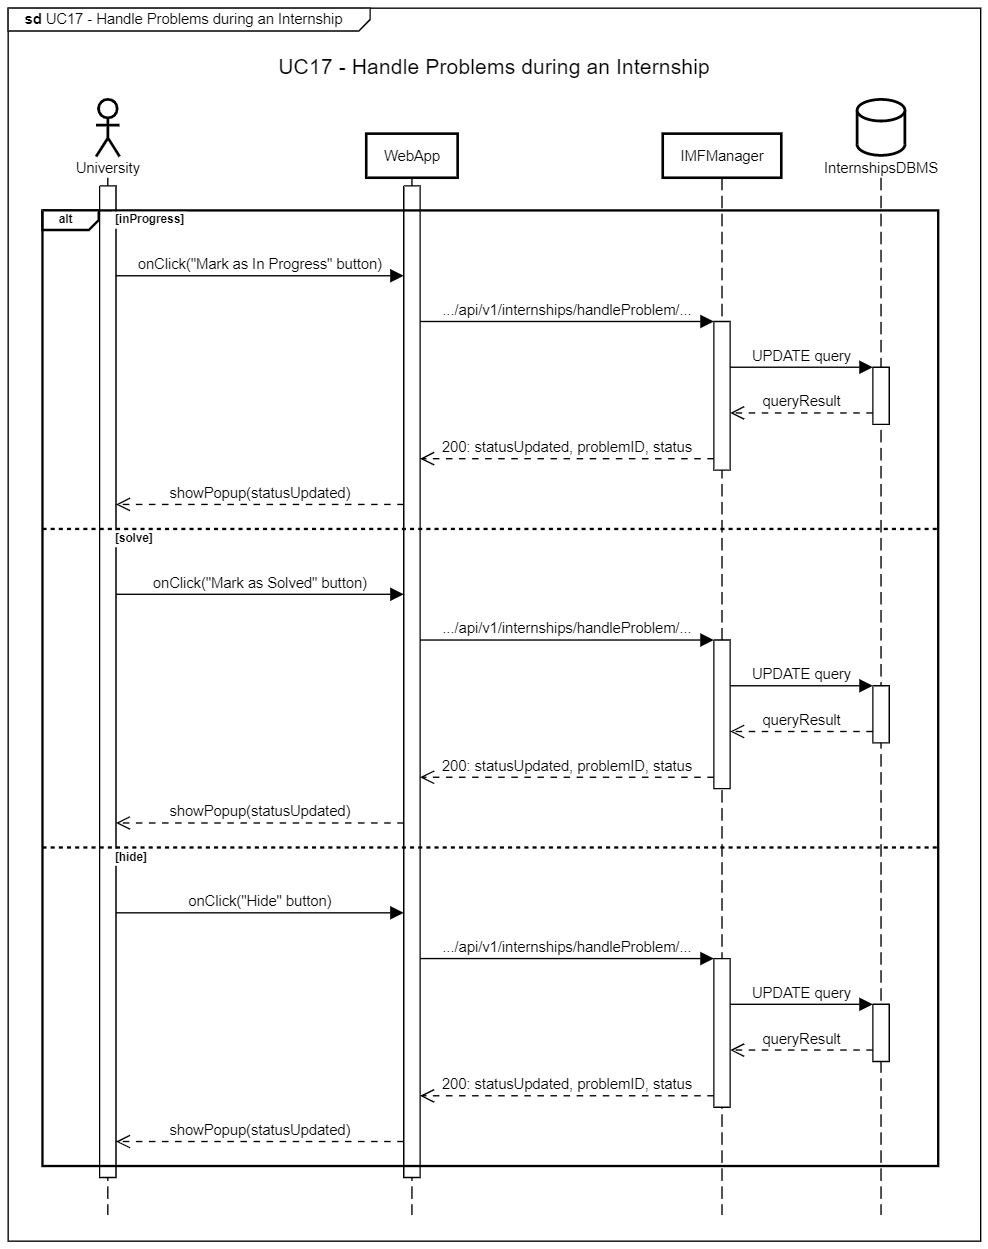
\includegraphics[width=0.75\linewidth]{LaTeXCode/images/SequenceDiagrams/UC17-sequenceDiagram.png}
         \caption{Handle Problems during an Internship}
         \label{fig:handle_problems_sd}
     \end{center}
\end{figure}

\newpage

\subsubsection*{SD\cuc. Report Feedback after an Internship}
\label{subsubsec:report_feedback_sd}
The Party begins by clicking the "Submit" button in the widget of an ended internship on their dashboard page, sending a request to the \texttt{.../api/v1/internships/reportFeedback/...} API handled by the \texttt{IMFManager}, which processes the request and updates the relevant records in the \texttt{InternshipsDBMS}. Once the feedback is successfully recorded, the \texttt{WebApp} is notified of the successful operation and displays a confirmation popup to the Party.

\begin{figure}[H]
    \begin{center}
         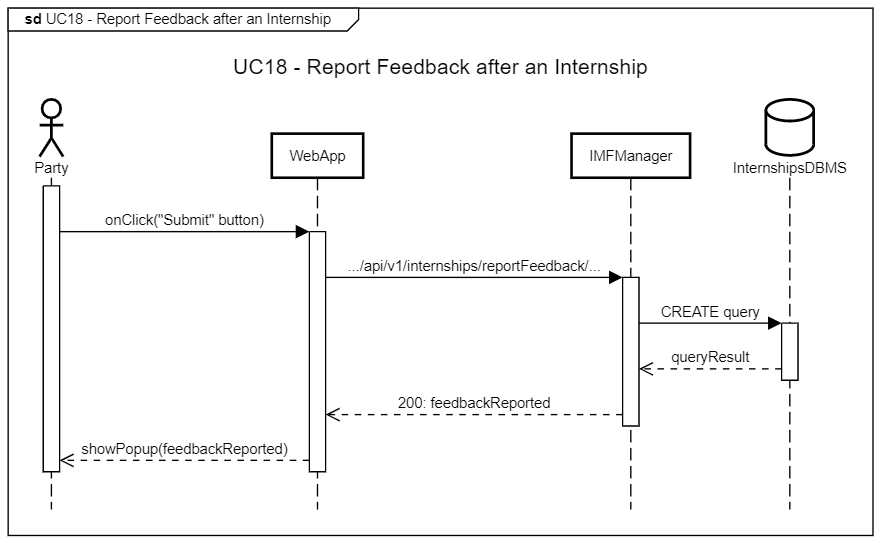
\includegraphics[width=1\linewidth]{LaTeXCode/images/SequenceDiagrams/UC18-sequenceDiagram.png}
         \caption{Report Feedback after an Internship}
         \label{fig:report_feedback_sd}
     \end{center}
\end{figure}

\newpage

\subsubsection*{SD\cuc. Suggest Optimizations for a Student Profile}
\label{subsubsec:suggest_optimizations_student_sd}
The Student initiates the action by clicking the "Improve Profile" button on their profile page, triggering a request to the \texttt{.../api/v1/optimizations/optimizeStudent/...} API endpoint, which is managed by the \texttt{OptimizationManager}. The \texttt{OptimizationManager} retrieves relevant data from the \texttt{RecommendationsDBMS} and processes the information to generate optimization suggestions. Once completed, the \texttt{OptimizationManager} sends the suggestions back to the \texttt{WebApp}, which displays them to the student.

\begin{figure}[H]
    \begin{center}
         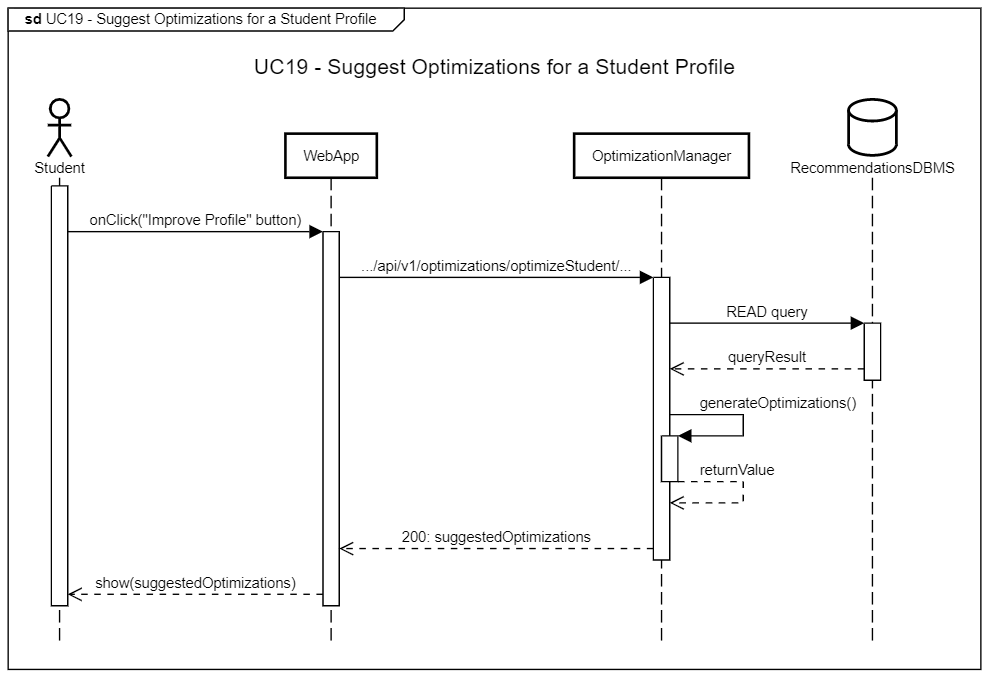
\includegraphics[width=1\linewidth]{LaTeXCode/images/SequenceDiagrams/UC19-sequenceDiagram.png}
         \caption{Suggest Optimizations for a Student Profile}
         \label{fig:suggest_optimizations_student_sd}
     \end{center}
\end{figure}

\newpage

\subsubsection*{SD\cuc. Suggest Optimizations for an Internship Offer}
\label{subsubsec:suggest_optimizations_internship_sd}
This Sequence Diagram is the same as the previous one, with the only difference being that it is started by a Company and not by a Student, and thus is about optimizing an offer and not a profile.

\begin{figure}[H]
    \begin{center}
         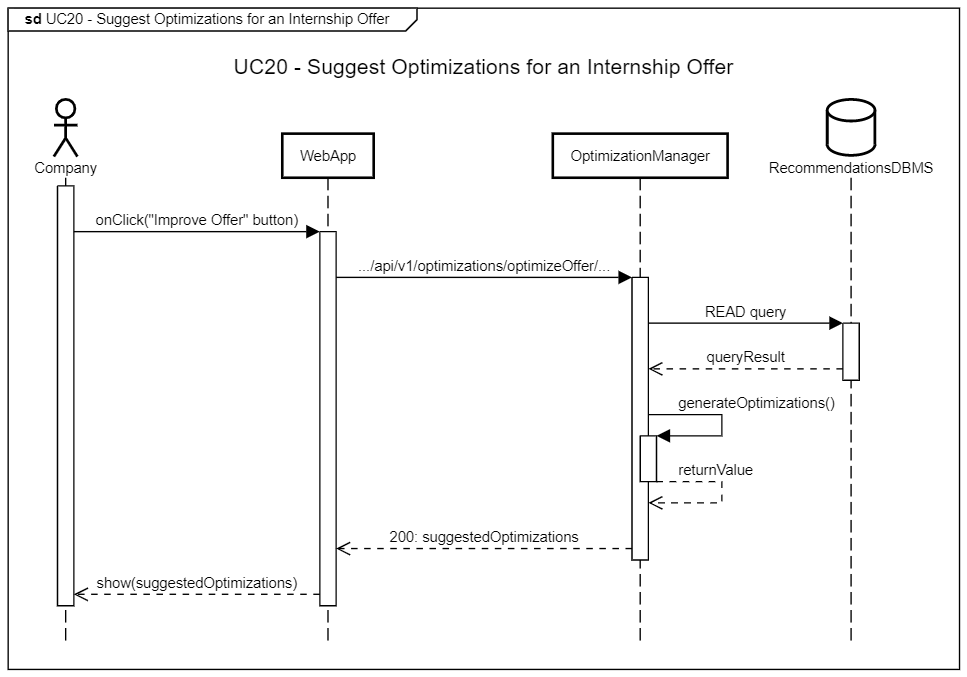
\includegraphics[width=1\linewidth]{LaTeXCode/images/SequenceDiagrams/UC20-sequenceDiagram.png}
         \caption{Suggest Optimizations for an Internship Offer}
         \label{fig:suggest_optimizations_internship_sd}
     \end{center}
\end{figure}

\newpage

\section{Selected Architectural Styles and Patterns}
\label{sec: patterns}%

For the S\&C system, various styles and patterns allow for better management of the key aspects of the system:

\begin{itemize}
    \item \textbf{Database-per-service pattern:} When implementing a system as a microservices architecture, it is strongly advised to partition the domain data according to the bounded contexts identified, obtaining one separate database for each service \hyperref[document: cloud_native_data_patters]{[3]}. This pattern comes with many advantages: independent scalability between the services, localized impact of schema evolutions or failures, and the possibility of using different technologies for distinct databases according to the needs of the specific domains. As a consequence, multiple databases are present in the S\&C system: the SecurityDB, the ProfilesDB, the InternshipsDB and the RecommendationsDB: for instance, if one of these databases goes down, the other microservices are not impacted at all.

    \item \textbf{Functional partitioning:} As just stated, data is partitioned among the various databases according to the bounded context of each microservice: in order to reduce cross-service queries to the bare minimum, bounded contexts have been identified as the different macro-functionalities that the system is required to offer, therefore adhering to a functional partitioning model \hyperref[document: data_partitioning]{[4]}. However, monitoring of the workload and distribution of data across all the databases should be constantly monitored, so that the database architecture can be redesigned as needed by performance issues, for example by adding horizontal partitioning (sharding) to the partitioning already in place.
    
    \item \textbf{Eventual consistency:} As the (in)famous CAP theorem states, it is impossible for a distributed system to achieve consistency, availability and partition tolerance (CAP) all at the same time \hyperref[document: relational_nosql_data]{[5]}. Given the choice of structuring the S\&C platform as a distributed system and the somewhat strict requirements on availability outlined in Section 3.5.2 \textit{Availability} of the RASD, the system is designed to be available and partition-tolerant alone, settling on only the eventual consistency of data across the spread-out databases and replicas. As the S\&C application is not handling critical processes, eventual consistency isn't really a problem \hyperref[document: data_consistency]{[6]}, as it doesn't matter if information about any offer isn't immediately up-to-date, or if a recommendation is not generated instantly after a new offer becomes available, or if some recommendations do not take into account the absolute latest information available.

    \item \textbf{Event Sourcing pattern:} A common choice to achieve data replication across a cluster of databases is implementing an event-driven architecture, also known as publish-subscribe: changes in the data one of the replicas generate events that get sent to all the other replicas. As stated before, tools based on the Raft protocol might be helpful: an example of such tools is Apache Kafka, which can be used as a channel to share the events between all the database copies. Kafka also supports multiple topics, enabling replication for different clusters of databases at the same time, and can also be configured to guarantee exactly-once semantics for ensuring events are not duplicated. Moreover, additionally to standard data replication, keeping data semantically separated comes with a cost, as some data is to be replicated across the different databases: this is the case for the RecommendationsDB, which is meant to gather data from the ProfilesDB and from the InternshipDB, representing something similar to what is called a \textbf{Materialized View}. As this can also be seen as a form of data replication, the standard Kafka distribution can also help: however, given that the involved databases are implemented with heterogeneous technologies, another suitable choice is to employ Kafka Connect with Change Data Capture (CDC), detecting changes in the databases by defining source connectors on the ProfilesDB and on the InternshipsDB and replicating them through a sink connector on the RecommendationsDB.

    \item \textbf{API Gateway pattern:} By introducing this pattern, the system establishes a single entry point for all client requests, unifying interactions with other components. Using NGINX, the system manages request routing to microservices and performs URL rewriting for necessary redirections. This approach enhances security by exposing only one public endpoint and optimizes internal traffic management. The benefits of adopting this pattern in our system include isolating clients from the internal partitioning of microservices, shielding them from the complexity of determining service instance locations, reducing the number of requests, and simplifying the client by shifting the logic for interacting with multiple services to the API Gateway \hyperref[document: api_gateway]{[7]}.

    \item \textbf{Circuit Breaker pattern:} In order for graceful degradation of the system to be completely achieved, it is necessary to take full advantage of the microservices architecture by implementing the Circuit Breaker pattern in the API Gateway directing the communications. In this way, microservices don't block or suffer from other services' slowdowns or failures, as the "link" between them can be opened and closed at will according to their current status, so that each service can keep functioning and offering limited functionalities also when it isn't able to make requests to another one.
\end{itemize}


    \chapter{User Interface Design}
    \label{ch:user_interface_design}%
    \section{General Overview}
\label{sec: general_overview}

The design of the user interfaces (UI) for the S\&C platform plays an important role in ensuring an engaging user experience. In the following section, through the use of possible UI interfaces, a comprehensive overview of the platform and its functionalities will be given, highlighting the principles and features that make the platform intuitive and accessible for its diverse user base.

The UI features a clean and consistent layout, obtained with uniform visual elements across pages and intuitive icons and labels, ensuring users can quickly find what they need and understand the differences between each section.

UI interfaces are not provided for every possible page described in the RASD \& DD documents, but only for the main pages which include the majority of the functionalities. Further interfaces can be made following the style provided in these layouts. Design choices, colors, fonts, and other elements can be modified accordingly in order to follow strategic business decisions to better engage the users.

Each webpage shown is responsive and adapts to all types of devices.

\newpage

\section{User Interfaces Layouts}
\label{sec: ui_layouts}

\subsection{Home Page}
\label{subsec: home_page}

\begin{figure} [H]
    \begin{center}
        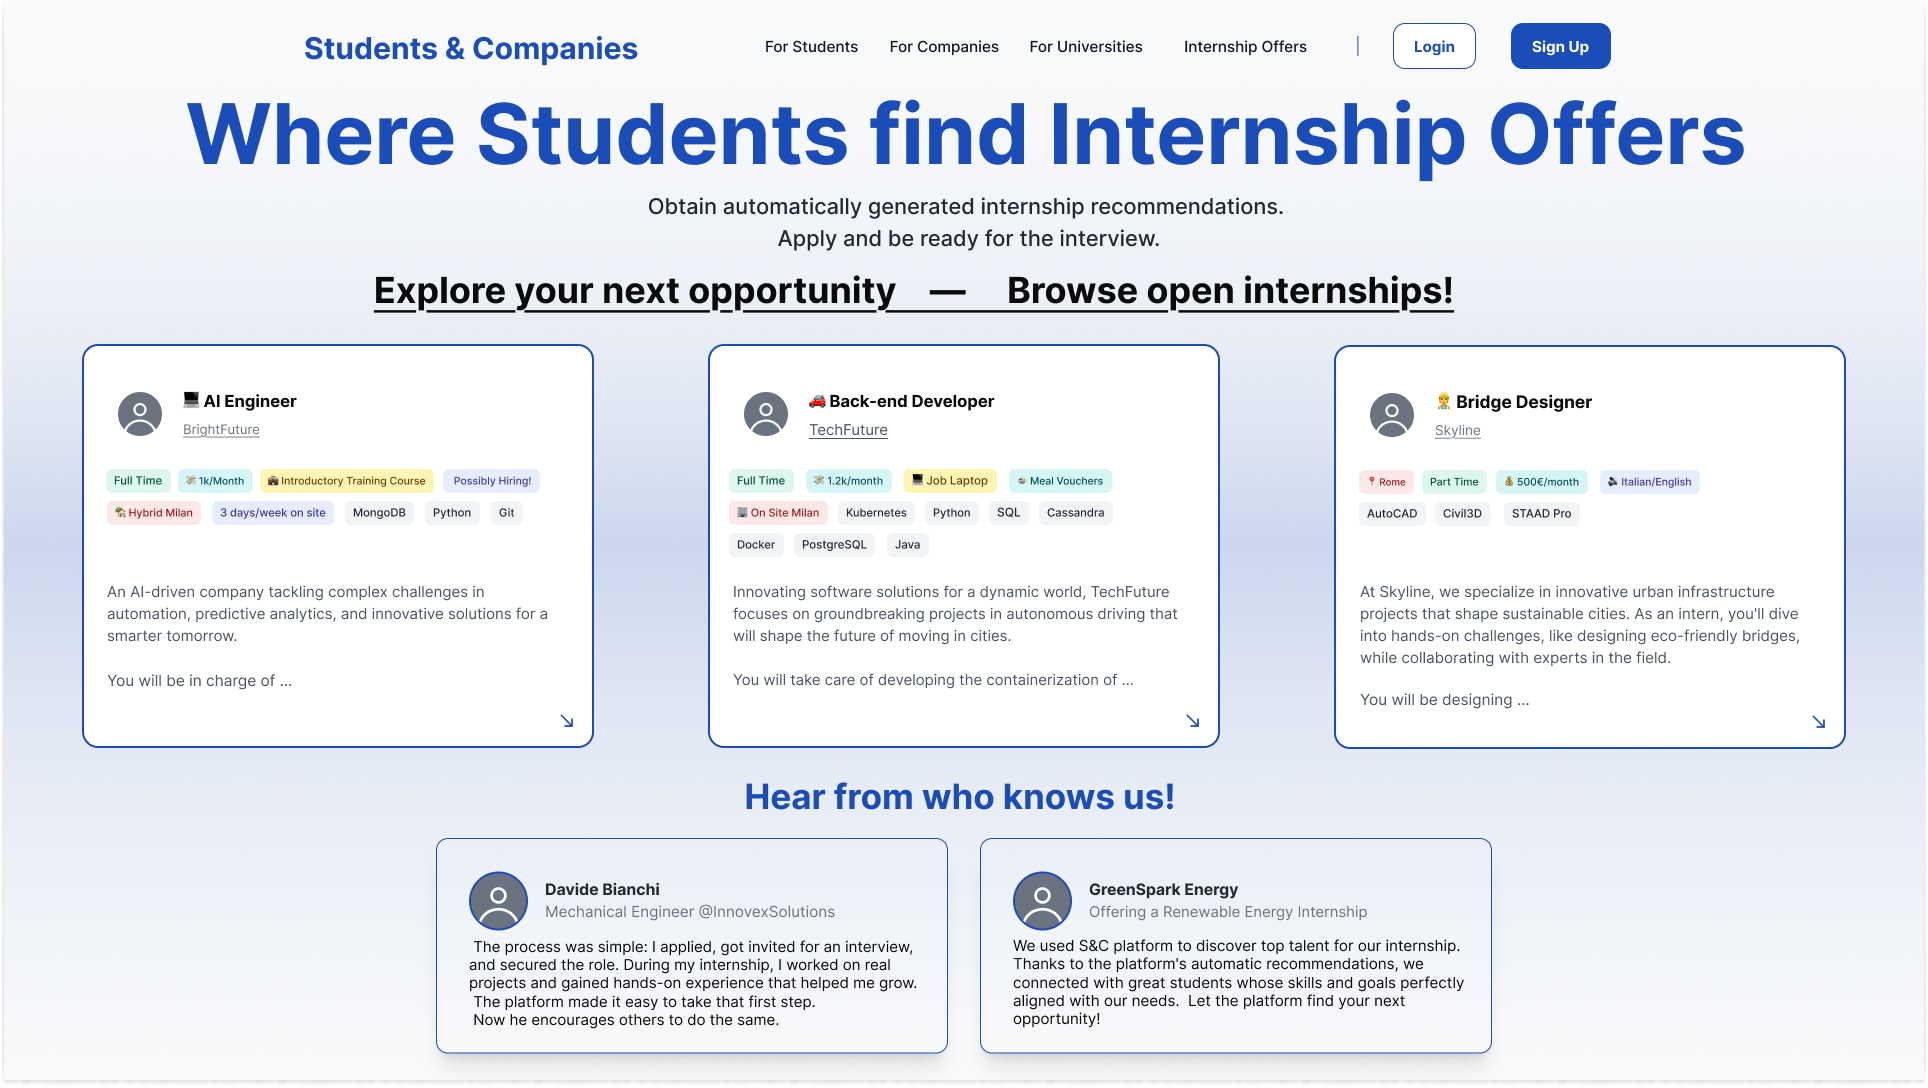
\includegraphics[width=0.9\linewidth]{LaTeXCode/images/UI/Homepage - Student.png}
        \caption{Landing Page of the WebApp}
        \label{fig: homepage}
    \end{center}
\end{figure}

The Home Page of S\&C is a multiple entry point for all the user groups. Its purpose is to guide students, companies, and universities to tailored content.
The navigation bar contains links to "For Students", "For Companies", "For Universities", which redirects to custom landing pages. In this case, the page displayed is specifically made for students.
The "Internship Offers" redirects to a browse-only carousel of internship offers, without any additional functionality prior to being registered.
The middle section displays some of the active internship opportunities in an interactive grid layout that can be manually moved by the user or automatically updates the showcased content after a certain time.
A testimonials section features true stories to build trust and credibility.
The page can also be extended vertically and made scrollable, to include more content and optionally a footer.

\subsection{Sign Up Page}
\label{subsec: sign_up_page}

\begin{figure} [H]
    \begin{center}
        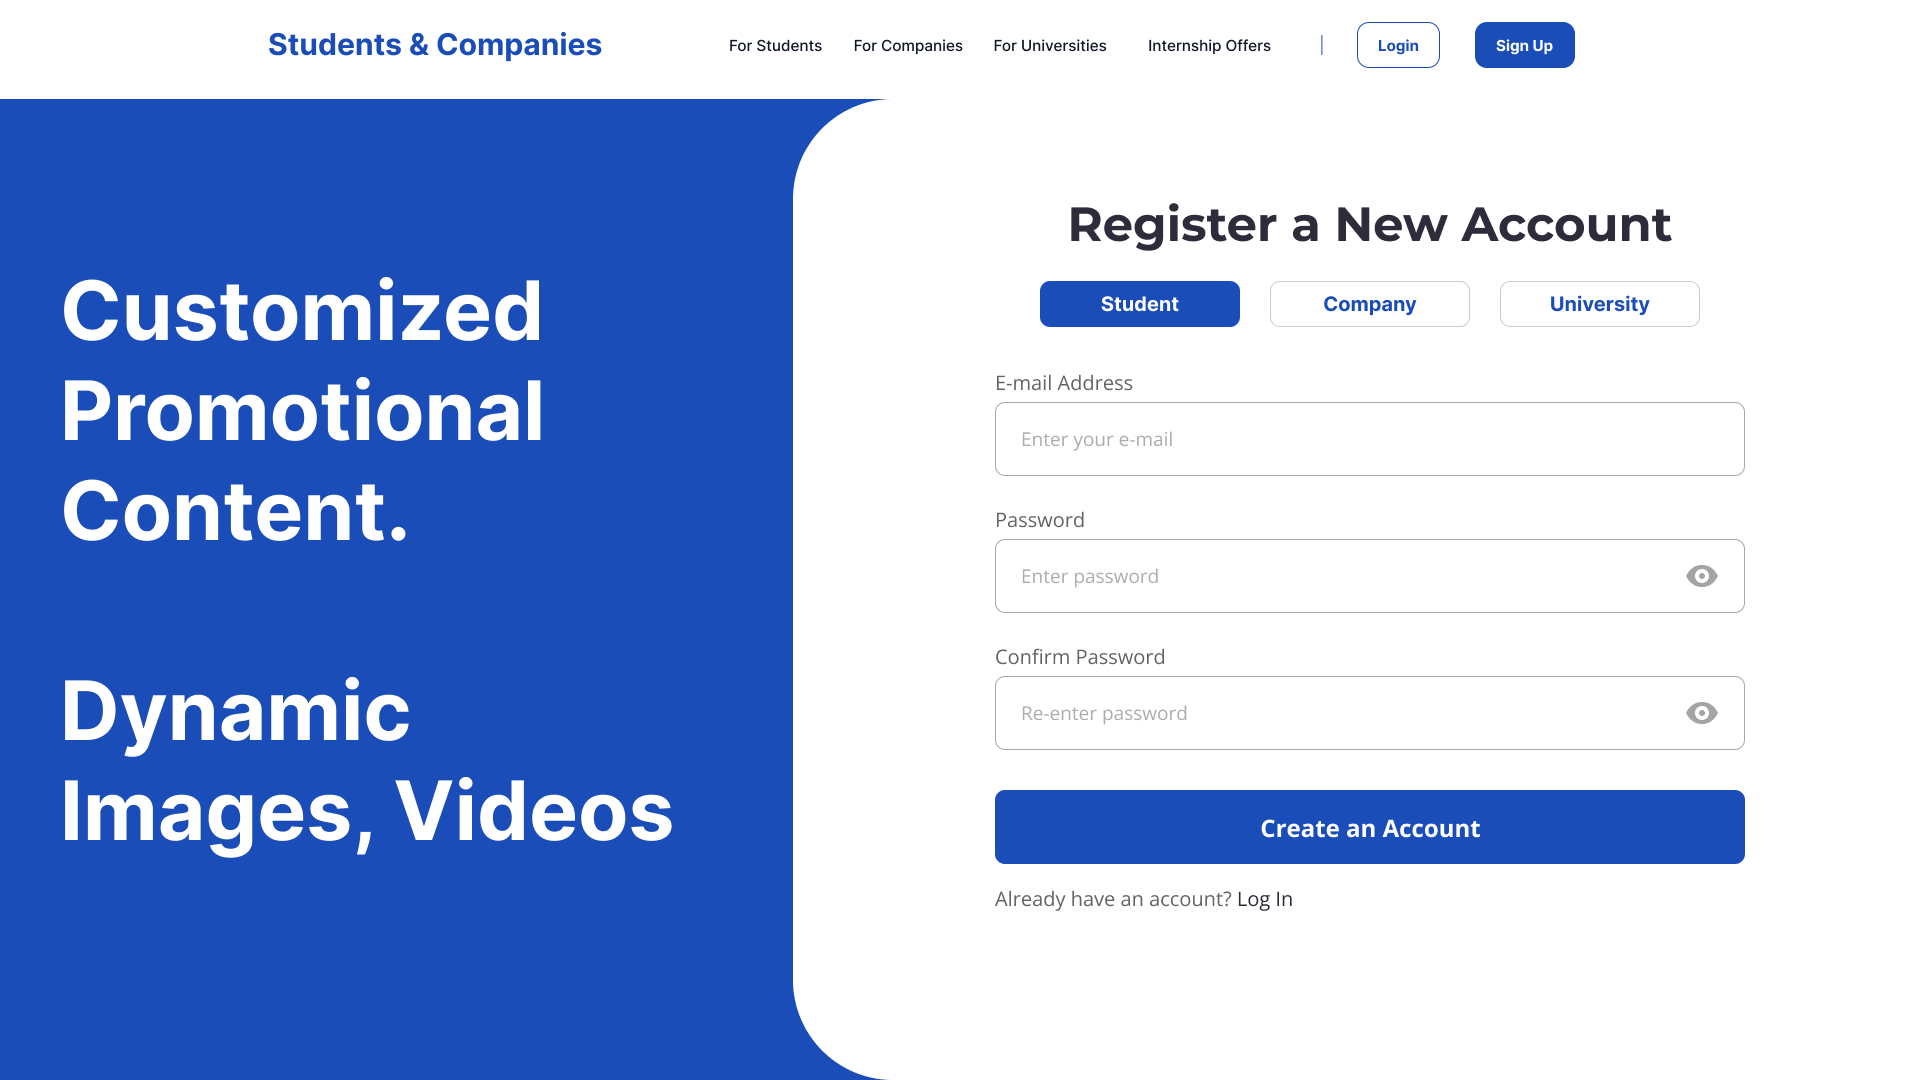
\includegraphics[width=0.9\linewidth]{LaTeXCode/images/UI/Sign Up - Unified Version.png}
        \caption{Sign Up - Initial Step}
        \label{fig: sign_up_unified}
    \end{center}
\end{figure}

The sign up page contains the initial step of the registration processes for all user groups. Additional information required to customize each profile will be collected in a subsequent form, accessible after the link in the confirmation email is accepted.
The navigation bar from the landing page remains consistently visible throughout the sign up process.

\subsection{Student Dashboard}
\label{subsec: student_dashboard}

The student dashboard contains all functionalities available to students. It is divided into three distinct views, accessible via a dropdown menu integrated into the navbar, only visible once a student is logged in.

\begin{figure} [H]
    \begin{center}
        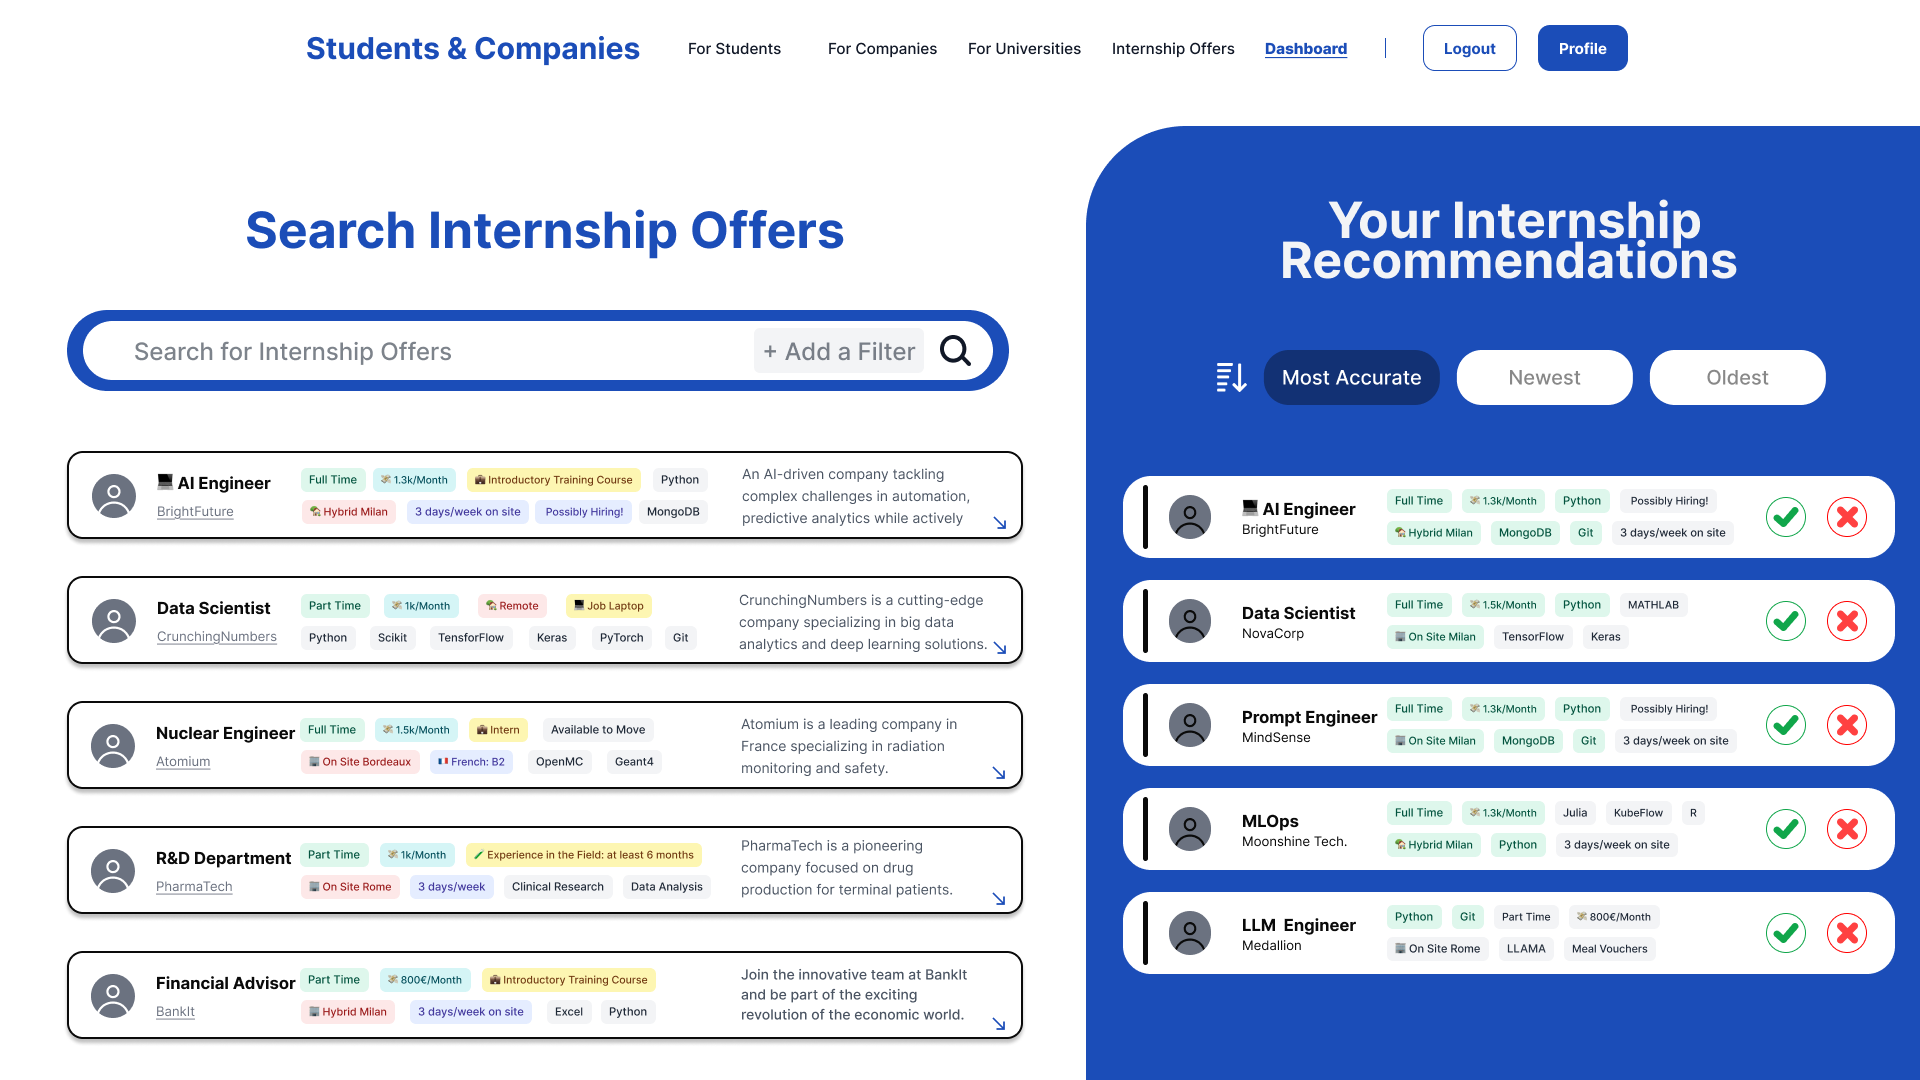
\includegraphics[width=0.9\linewidth]{LaTeXCode/images/UI/Student Dashboard - Main View.png}
        \caption{Student Dashboard - Main View}
        \label{fig: dashboard_student_main}
    \end{center}
\end{figure}

The main view, displayed by default whenever a student is redirected to the dashboard, is made by two sections: Search Internship Offers and Your Internship Recommendations.

On the left, the search functionality allows students to explore internship offers using a text-based search bar. The search can be further refined with predefined filters, such as keywords found in posted internship descriptions. If no input is provided, the system displays a random selection of internship offers. After initiating a search, the results appear in a vertical list layout. Each internship offer is an interactive element that opens a modal to display detailed information and includes the option to apply directly.

On the right, the Recommendations section shows the internship recommendations automatically generated by the system. Students can choose to accept or decline these recommendations and sort them based on predefined criteria, as indicated by the three intuitive sorting buttons. Each recommendation is interactive, allowing students to view offer details via a modal. 
As previously detailed in the document, students can apply directly through the internship offers or the recommendations with identical technical functionality.

Both sections are dynamic and adapt in real-time to user interactions.

\begin{figure} [H]
    \begin{center}
        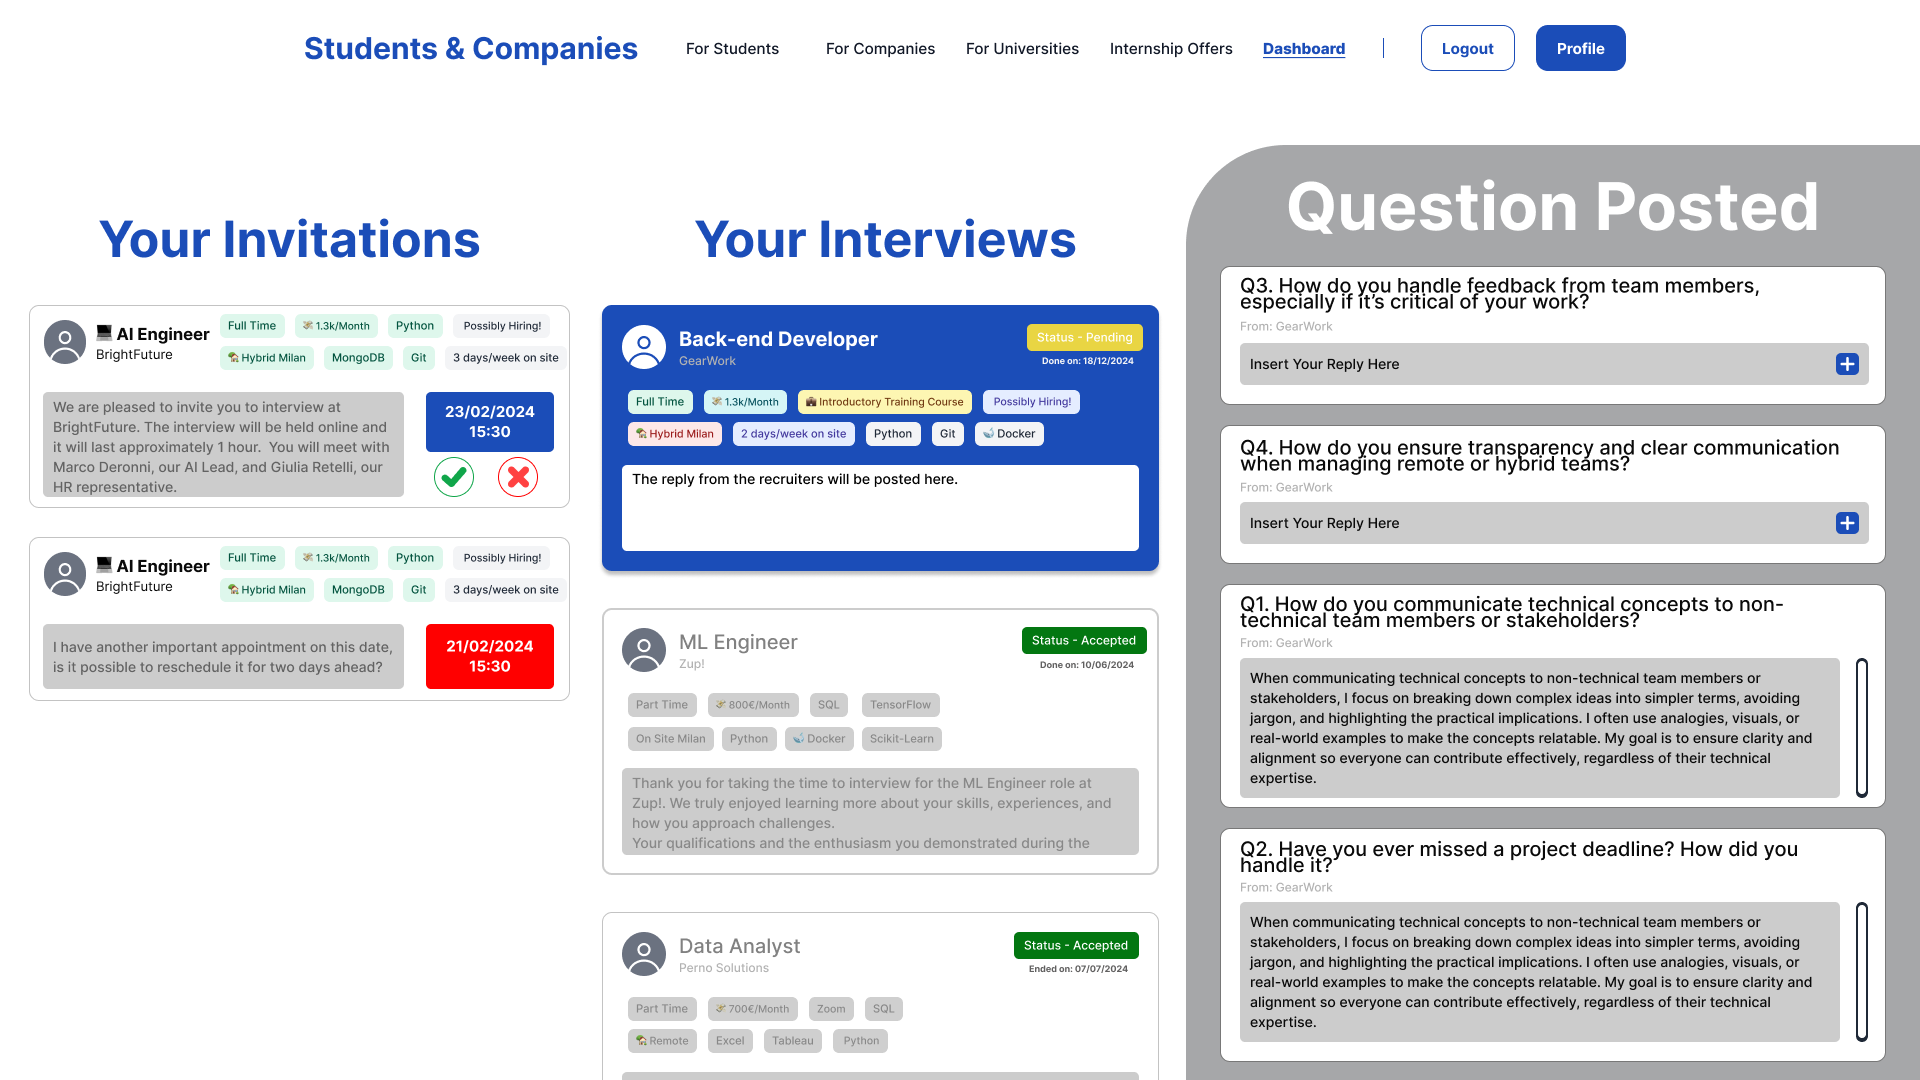
\includegraphics[width=0.9\linewidth]{LaTeXCode/images/UI/Student Dashboard - Second View.png}
        \caption{Student Dashboard - Second View}
        \label{fig: dashboard_student_second}
    \end{center}
\end{figure}

The second view, accessible through the drop-down menu, contains all the functionalities related to interviews and is divided into three sections: Your Invitations, Your Interviews, and a Message Board for questions related to the internships you have applied for.

On the left side, the Your Invitations section displays all pending, accepted, and refused interview invitations for internship offers where the interview process is still ongoing. Invitations are sorted chronologically, with the most recent ones appearing at the top. If a student declines an invitation, a modal will appear, asking to provide a reason or message to the hiring company.

The middle section, Your Interviews, lists all completed interviews. Each entry includes a summary of the position applied for, the interview date, and the current status of the application. 
When the company ends the process, feedback from the recruiter is displayed within each interview entry. Similar to the Invitations section, interviews are organized chronologically from top to bottom.

On the right side, the Message Board displays questions posted by companies conducting interviews for the internships you’ve applied to. Unanswered questions are shown at the top, while those you’ve already responded to appear below. Since questions from different companies may appear in a mixed layout, each question identifies the company that posted it. Alternatively, a filtering option by company can be added to obtain a separated view for each company. Once a selection process is completed, associated questions are automatically removed from the board.

\begin{figure} [H]
    \begin{center}
        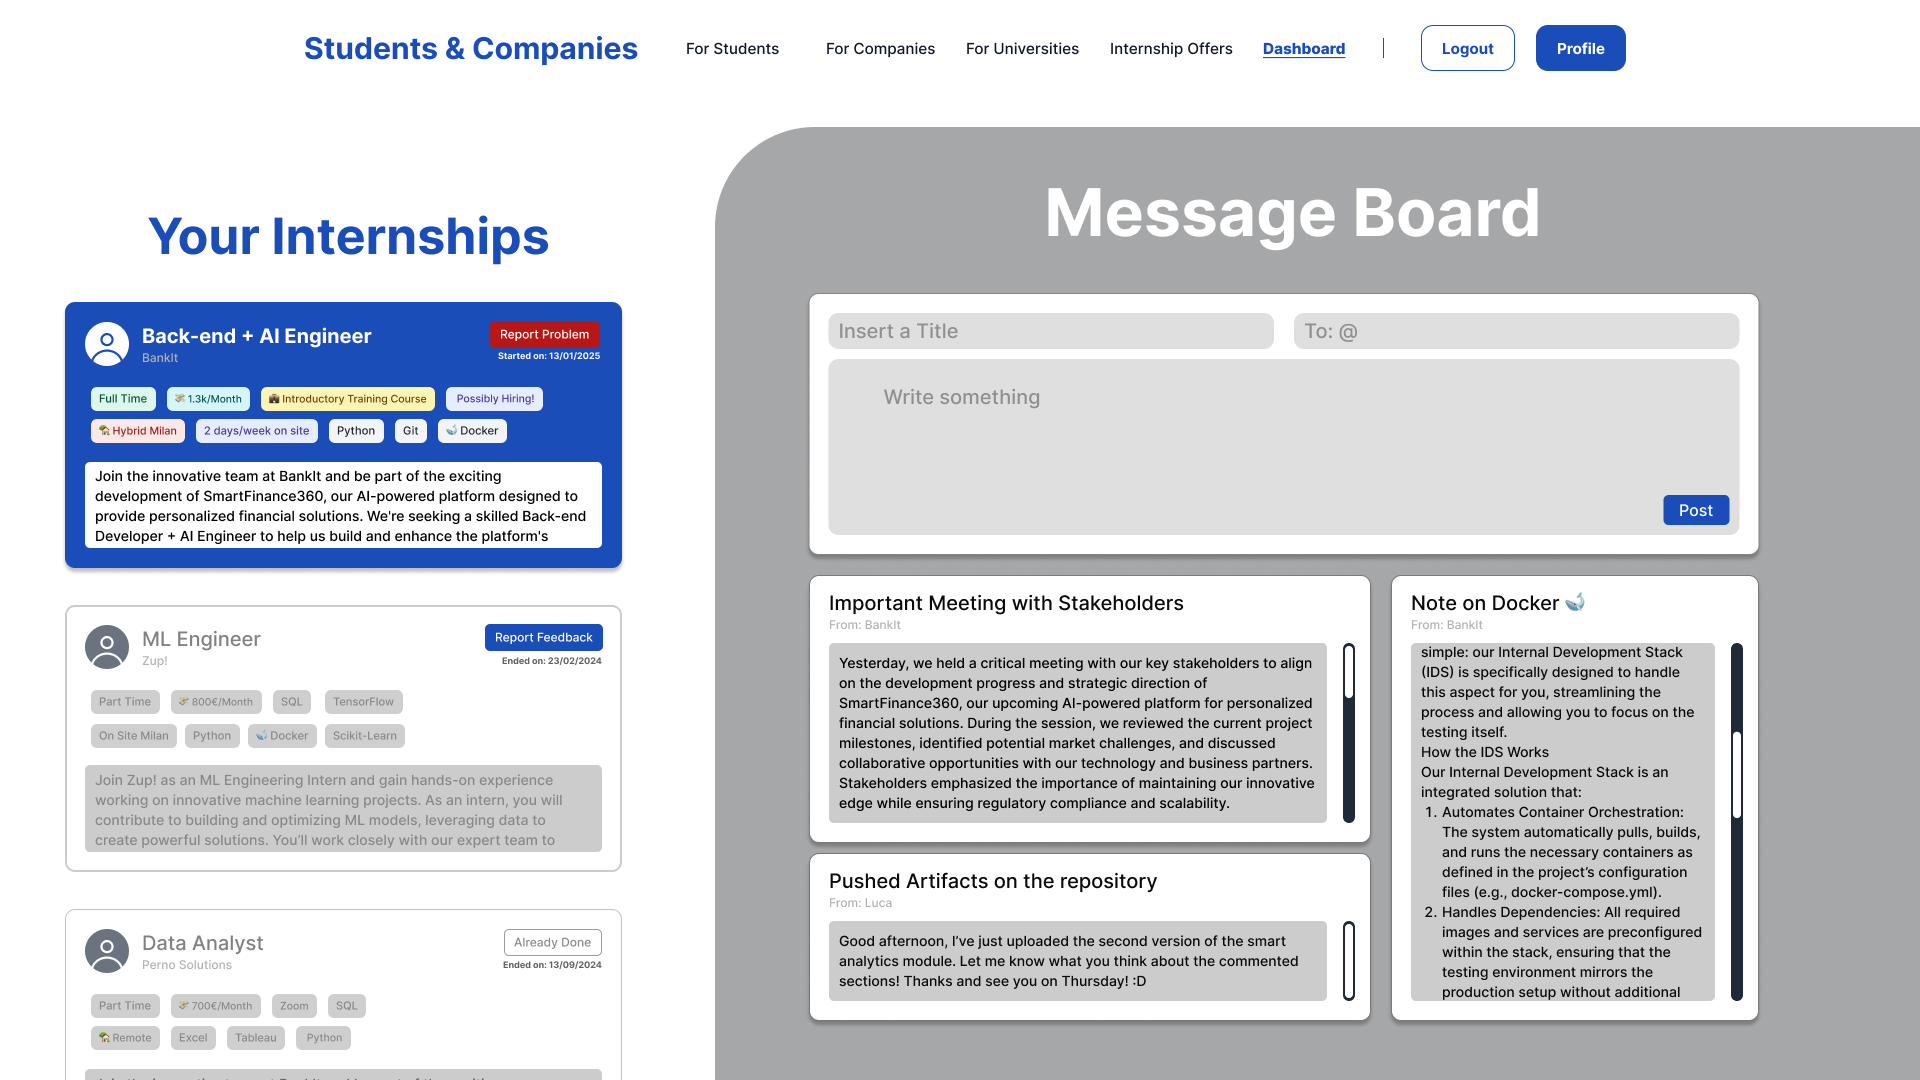
\includegraphics[width=0.9\linewidth]{LaTeXCode/images/UI/Student Dashboard - Third View.png}
        \caption{Student Dashboard - Third View}
        \label{fig: dashboard_student_third}
    \end{center}
\end{figure}

The third view, accessible through the dropdown menu, provides all functionalities related to ongoing and completed internships, organized into two sections: Your Internships and a Message Board for communication with the company.

On the left, the Your Internships section displays details of both ongoing and completed internships. Each ongoing internship includes a summary of the applied position, the starting date, and a "Report Problem" feature that initiates a process managed by the university to address issues. Completed internships are also listed here, with the option to provide feedback if it has not already been submitted. As in other sections, internships are sorted chronologically, with the most recent at the top.

On the right, the Message Board provides a dedicated space for displaying all communications between the student(s) and the company. At the top, students can post new messages, while previous messages are displayed below in chronological order. Older messages can be accessed by scrolling further down the section, ensuring all messages remain accessible.

\subsection{Profile Page - Student}
\label{subsec: profile_page_student}

\begin{figure} [H]
    \begin{center}
        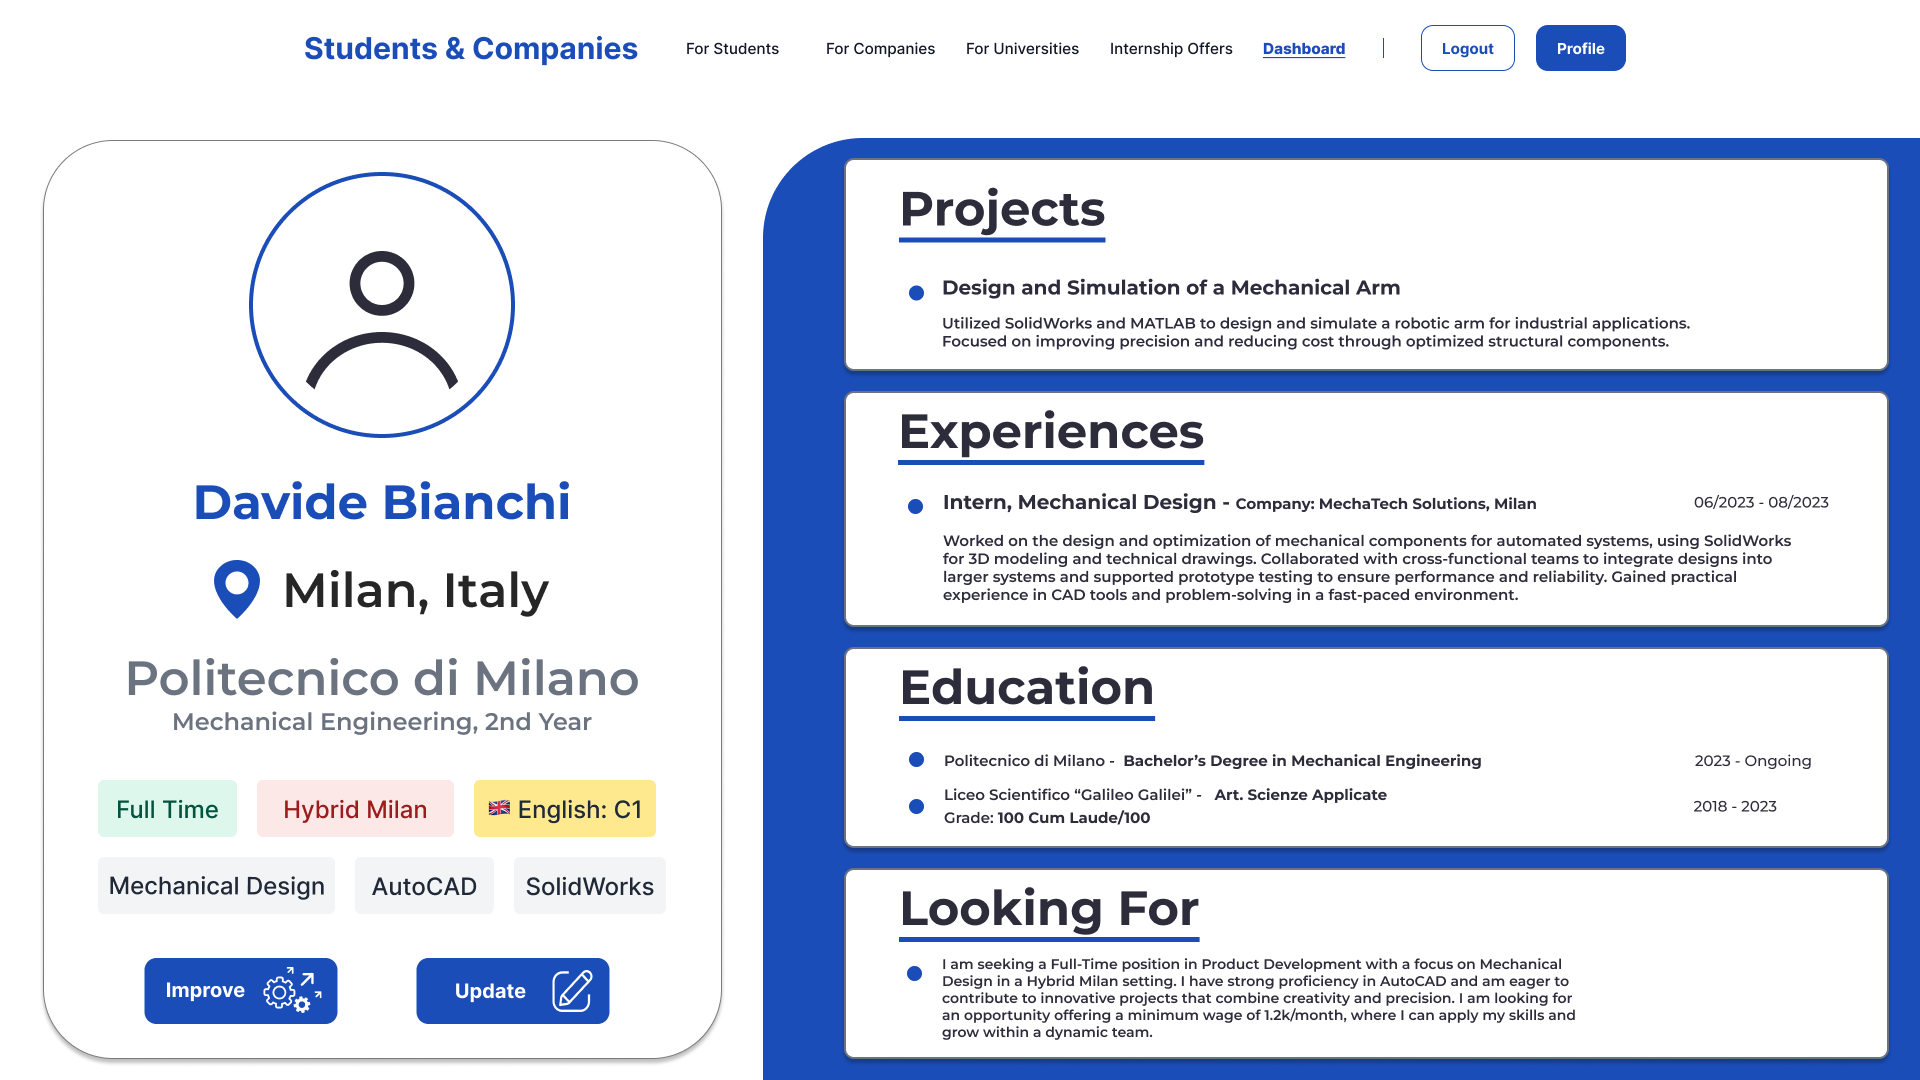
\includegraphics[width=0.9\linewidth]{LaTeXCode/images/UI/Student Dashboard - Profile.png}
        \caption{Profile Page - Student}
        \label{fig: profile_student}
    \end{center}
\end{figure}

The Profile page, accessible through the navigation bar, contains all information related to the student.

On the left, a summary of the student’s profile is displayed, highlighting the most relevant details along with a subset of keywords extracted from their complete profile. Below this summary, two key actions are available: Suggest Optimizations for a Student Profile, which provides recommendations to enhance the profile, and Update Profile, allowing students to edit their information.

On the right, the main subsections of the curriculum are presented. These sections are used to identify and extract keywords that define the student's keywords.

Other profile pages expected in the platform, for Company and University, are similar in the general layout and only differ in the content shown, and so for this reason their UI is not provided in this document.

\subsection{Company Dashboard}
\label{subsec: company_dashboard}

The company dashboard contains all functionalities available to companies. It is divided into three distinct views, accessible via a dropdown menu integrated into the navbar, only visible once a company is logged in.

\begin{figure} [H]
    \begin{center}
        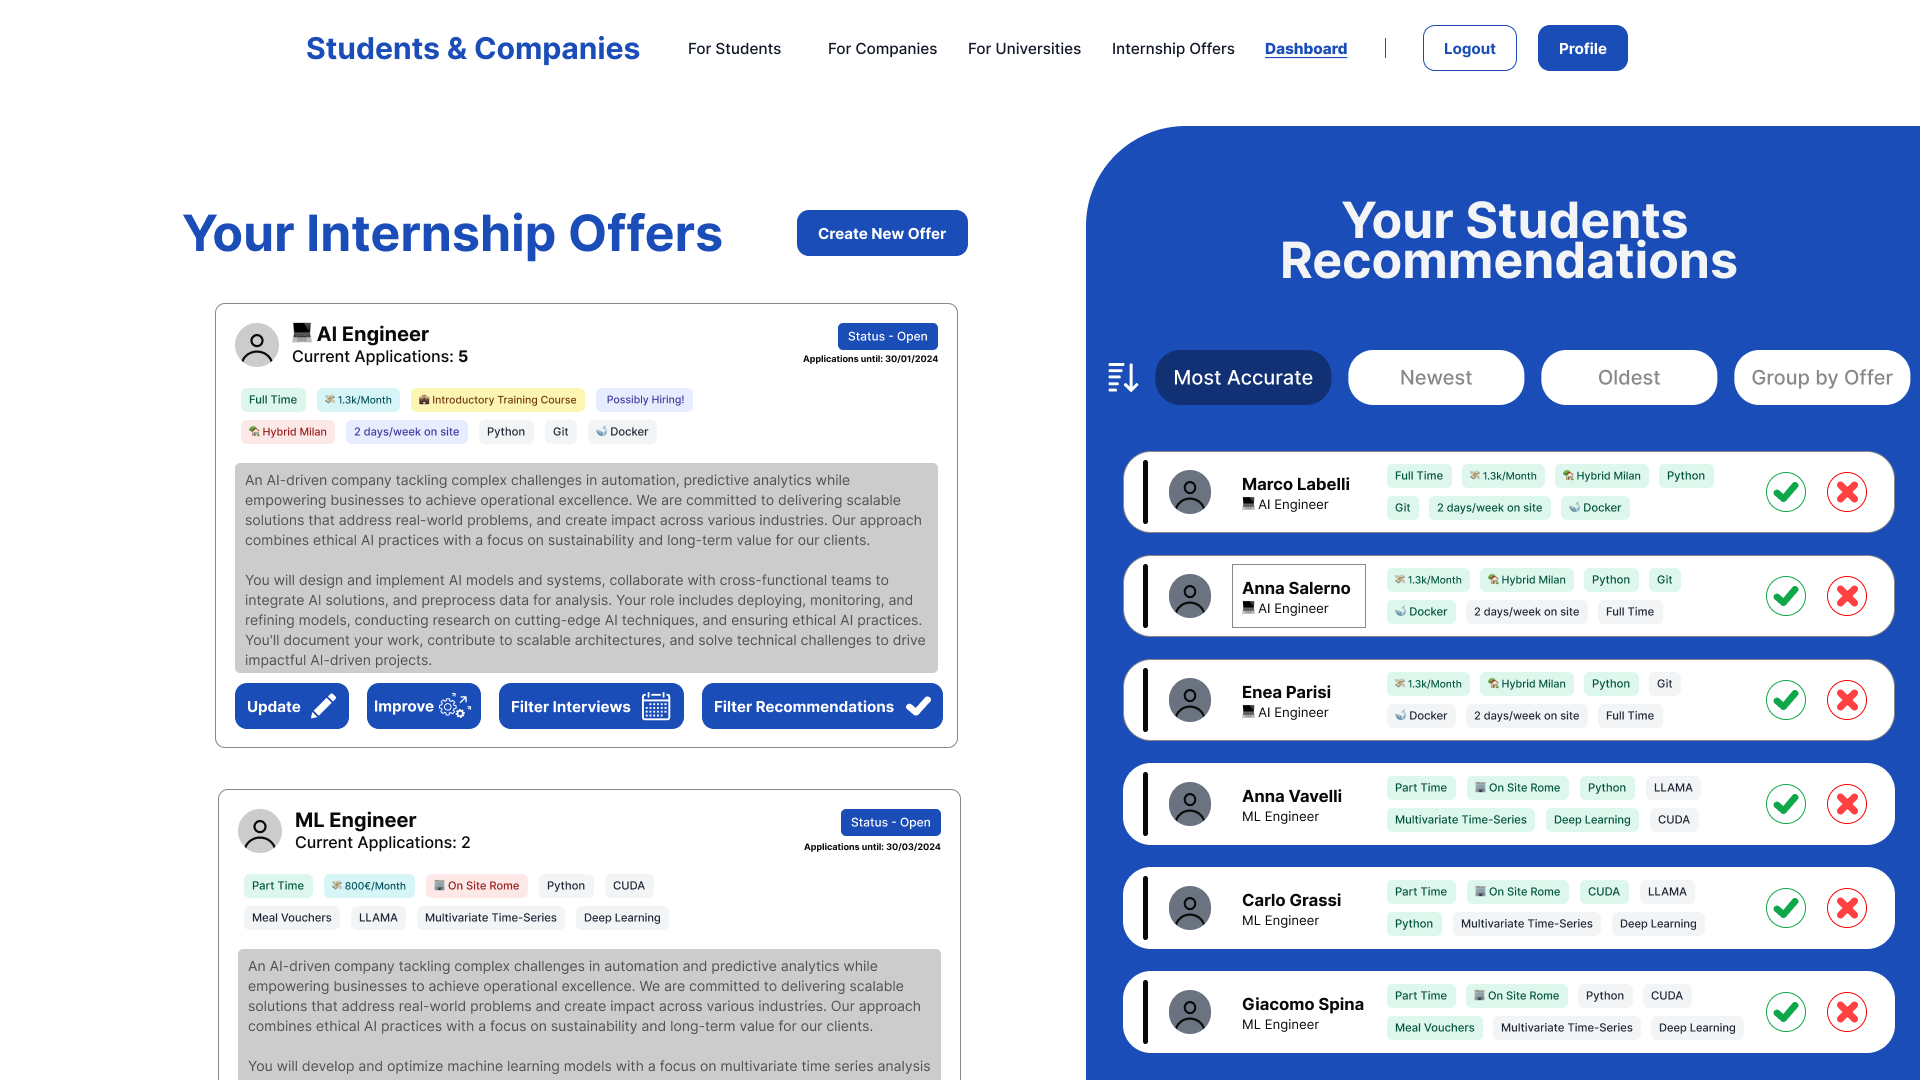
\includegraphics[width=0.9\linewidth]{LaTeXCode/images/UI/Company Dashboard - Main View.png}
        \caption{Company Dashboard - Main View}
        \label{fig: dashboard_company_main}
    \end{center}
\end{figure}

The main view, displayed by default whenever a company is redirected to the dashboard, is composed of two sections: Your Internship Offers and Your Students Recommendations.

On the left, all open internship offers are listed, displaying the description provided during posting and relevant keywords extracted from the description.
To perform the insertion of a new internship offer on the platform, companies can use the associated button, which opens a modal containing a form with all the required fields to be compiled.
Each internship is an interactive element that can be expanded into a modal for detailed visualization, including its description and a list of applicants. Below each internship, there are further options: one to edit the offer's details or eventually withdraw it and another to receive suggestions for improving its content. A Filter Interviews button allows navigation to the Interviews section of the dashboard, focusing exclusively on interviews and invitations for that specific offer. By default, the Interviews section displays invitations and interviews for all internships currently in the Selection phase. Additionally, a Filter Recommendations button performs a similar action, filtering the Recommendations section (on the right) to suggestions relevant to the selected internship.

On the right, the Recommendations section shows the student recommendations automatically generated by the system. Companies can accept or decline these recommendations and sort them using four intuitive sorting buttons. Each recommendation highlights the compatibility between internship offer keywords and student profiles. Recommendations are interactive, enabling companies to view detailed student profiles through a modal.

\begin{figure} [H]
    \begin{center}
        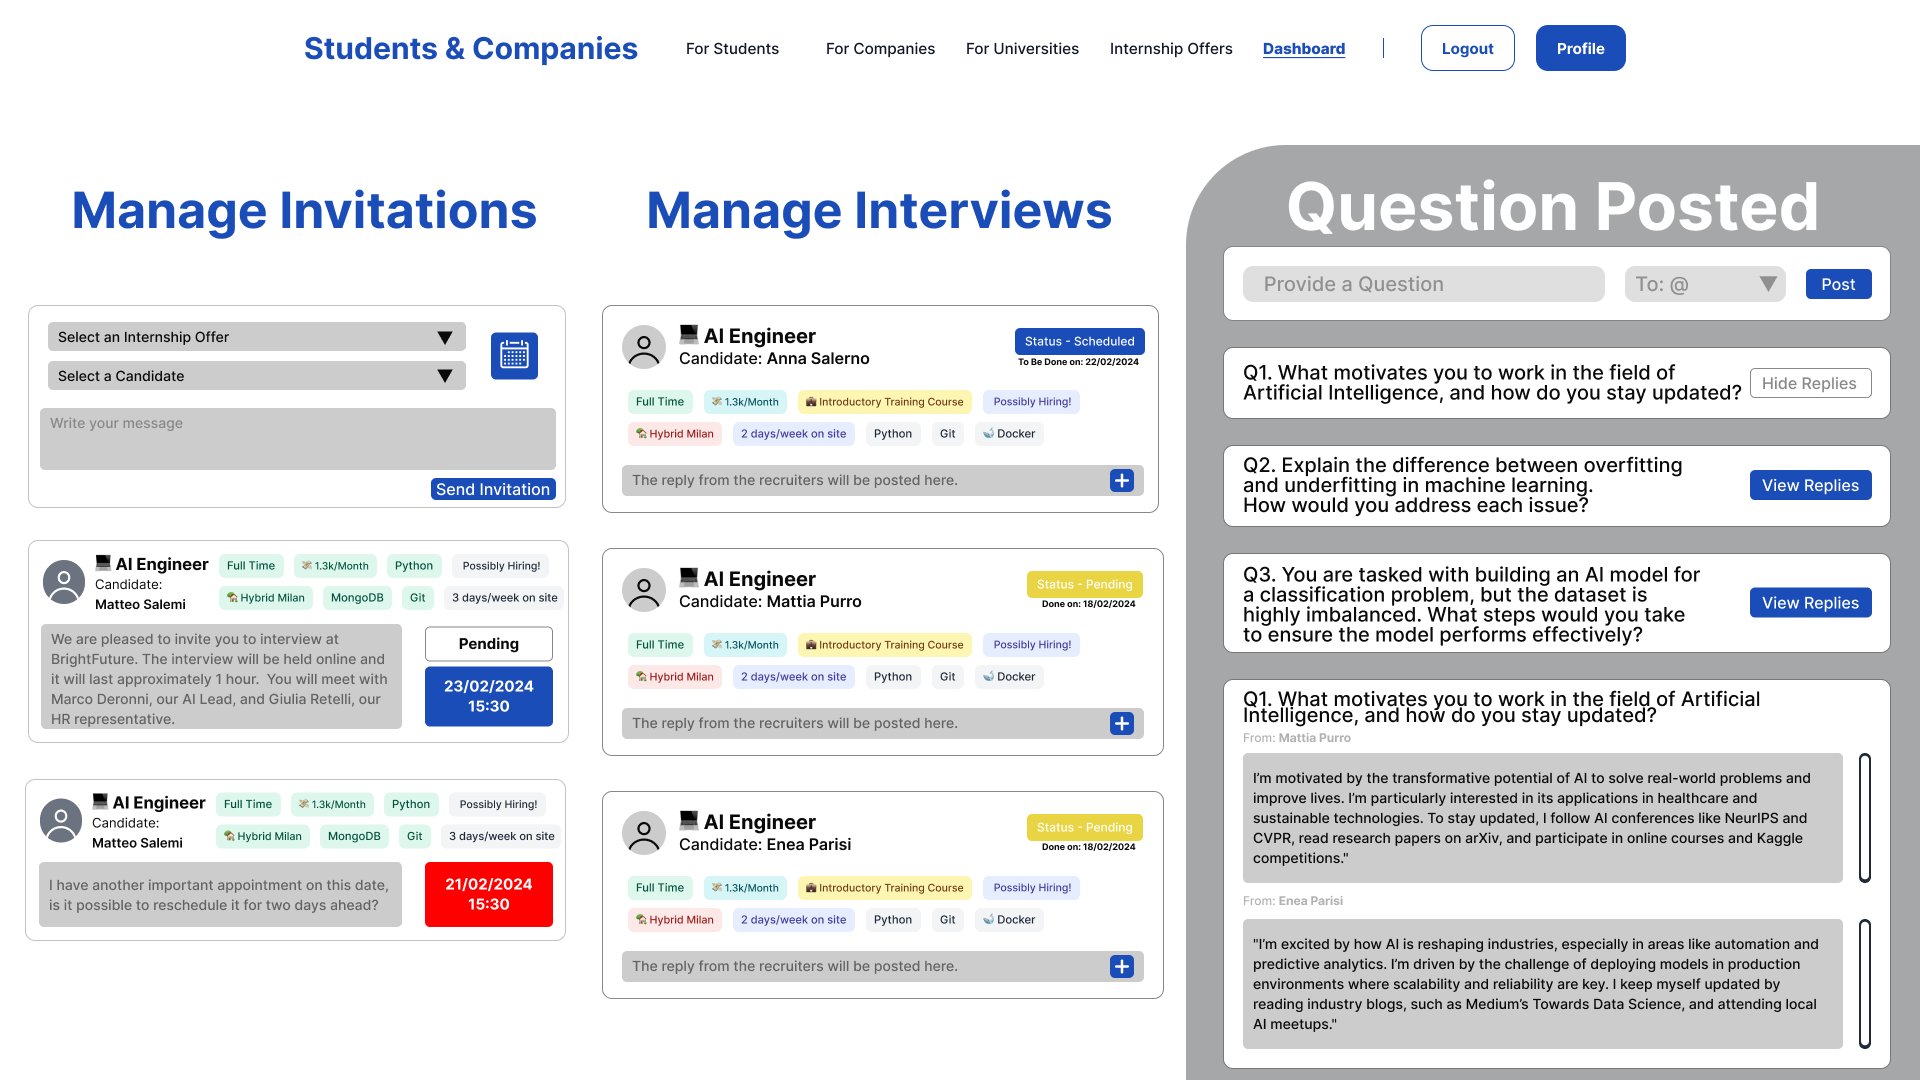
\includegraphics[width=0.9\linewidth]{LaTeXCode/images/UI/Company Dashboard - Second View.png}
        \caption{Company Dashboard - Second View}
        \label{fig: dashboard_company_second}
    \end{center}
\end{figure}

The second view, accessible via the drop-down menu or the previously mentioned shortcut, contains all functionalities related to interviews. It is divided into three sections: Manage Invitations, Manage Interviews, and a Message Board for providing questions to candidates during interviews.

On the left, companies can create new invitations by selecting the associated internship offer and choosing a candidate from a dropdown menu, specifying a proposed date and time, and providing a description. Below this, all refused and pending invitations are displayed, while accepted invitations automatically move to the middle section.

The middle section shows all scheduled interviews, sorted chronologically. Here, companies can provide feedback on each interview, which includes a status field that can be updated by clicking on it to finally accept or decline the candidate.

On the right, the Message Board allows companies to post new questions to candidates, selecting one or multiple candidates through a dropdown menu. Companies can also monitor replies to previous questions, with options to view or hide specific questions using dedicated buttons.

\begin{figure} [H]
    \begin{center}
        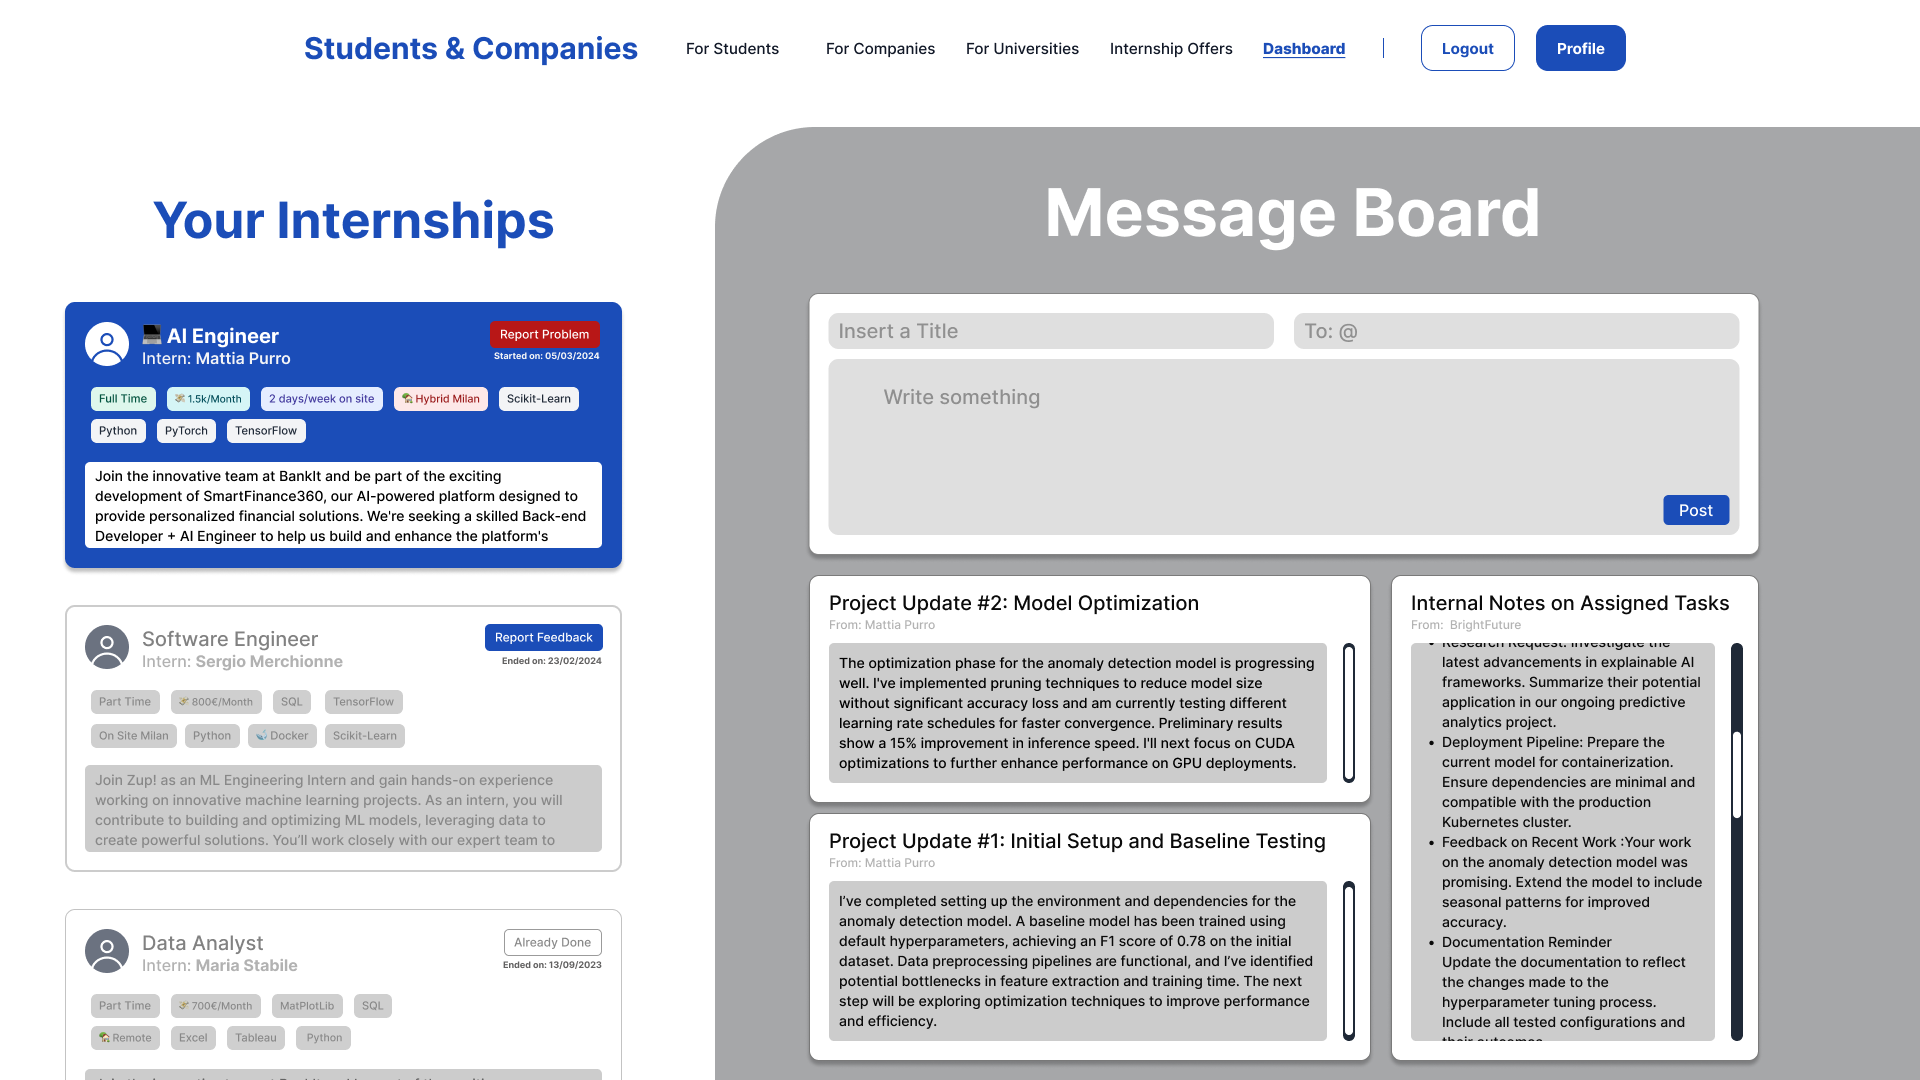
\includegraphics[width=0.9\linewidth]{LaTeXCode/images/UI/Company Dashboard - Third View.png}
        \caption{Company Dashboard - Third View}
        \label{fig: dashboard_company_third}
    \end{center}
\end{figure}

The third view, accessible through the dropdown menu, provides all functionalities related to ongoing and completed internships, organized into two sections: Your Internships and a Message Board for communication with the students.

On the left, the Your Internships section displays details of both ongoing and completed internships. Each ongoing internship includes a summary of the applied position, the starting date, and a "Report Problem" feature that initiates a process managed by the university to address issues. Completed internships are also listed here, with the option to provide feedback if it has not already been submitted. As in other sections, internships are sorted chronologically, with the most recent at the top.

On the right, the Message Board provides a dedicated space for displaying all communications between the company and the student(s). At the top, companies can post new messages, while previous messages are displayed below in chronological order. Older messages can be accessed by scrolling further down the section, ensuring all messages remain accessible.

\subsection{University Dashboard}
\label{subsec: university_dashboard}

The university dashboard contains all functionalities available to universities. It is composed of a minimal view, accessible via the dashboard link integrated into the navbar, only visible once a university is logged in.

\begin{figure} [H]
    \begin{center}
        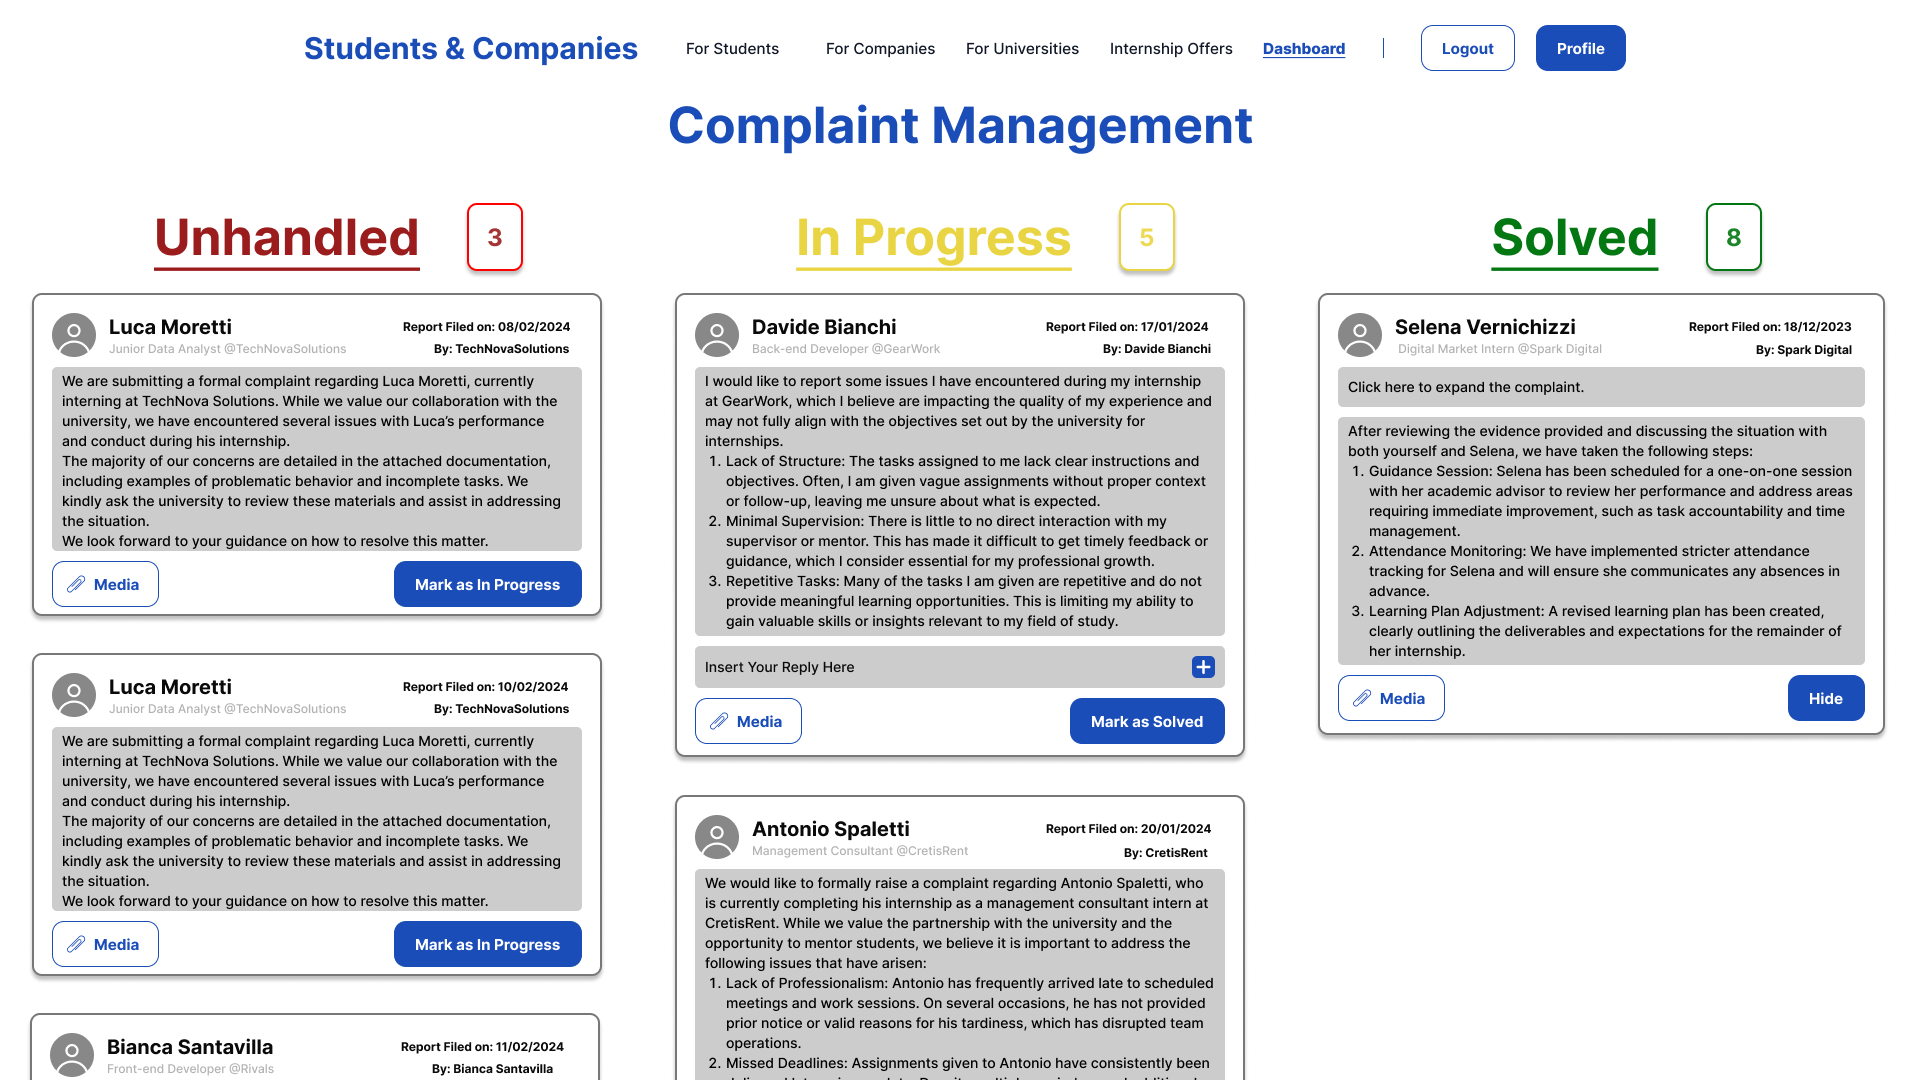
\includegraphics[width=0.9\linewidth]{LaTeXCode/images/UI/University Dashboard - Complaint Management View.png}
        \caption{University Dashboard - Complaint Management View}
        \label{fig: dashboard_university_complaint}
    \end{center}
\end{figure}

The default view, displayed whenever a university is redirected to the dashboard, consists of three sections that form the Complaint Management Dashboard. This dashboard enables the university to execute the "Handle Problems" functionality for their students.

The layout is intuitive, featuring a three-column pipeline that organizes complaints based on their status: Unhandled, In Progress, or Solved. Complaints are displayed in reverse chronological order within each column, with the oldest reports at the top and the newer ones below.

Each report includes comprehensive details about the student, their role, the date the report was filed, and the reporting party. A description of the issue is presented in a dedicated text section, and any attached media can be accessed by clicking the Media button.

When the status of a report changes, it automatically moves to the corresponding adjacent column. Once a report is marked as solved, the university has the option to hide it from the dashboard view to reduce clutter.

To improve focus, the university can hide any of the three columns by clicking the corresponding label. The remaining columns will dynamically adjust to occupy the available space equally.



    \chapter{Requirements Traceability}
    \label{ch:requirements_traceability}%
    This chapter shows how the functional and non-functional requirements of the S\&C system described in the RASD are mapped to each component.
First, we describe the mapping between the requirements listed in Section 2.2.1. \textit{Requirements} of the RASD document
and the components identified in the Component Diagram section of the DD document.
Then, we comment on how Sections 3.3 \textit{Performance Requirements} and 3.5 \textit{Software System Attributes} of the RASD document are achieved through the decisions taken for the S\&C system.

\section{Functional Requirements Traceability}
\label{sec: functional_requirements_traceability}
The following table lists all the requirements linked within each component.
\begin{center}
    \begin{longtable}{p{0.3\linewidth}p{0.7\linewidth}}
        \hline
        \textbf{MailingService}                 & [R1]\ Upon request, the system shall allow the User to sign up to the platform, as long as they submit all the required information, they don’t already have a profile in the platform and their identity and role (Student, Company or University) are verified. \\ \\
        \hline
        \textbf{SecurityManager}                 & [R1] Upon request, the system shall allow the User to sign up to the platform, as long as they submit all the required information, they don’t already have a profile in the platform and their identity and role (Student, Company or University) are verified. \\ \\
        & [R2] Upon request, the system shall allow the requesting User to log in to the platform, granting him access to their profile as long as their authentication is successful. \\ \\
        \hline
        \textbf{ProfileManager}             & [R3] Upon request, the system shall allow the requesting User to update their profile, as long as they provide all the necessary information. \\ \\
        \hline
        \textbf{OfferManager}                        & [R4] Upon request, the system shall allow a Company to publish a new internship offer, as long as it provides all the required information and the latter is compliant with platform guidelines. \\ \\     
        & [R5] Whenever a Company publishes an internship offer, the system shall add it to the list of all the internship offers. \\ \\
        & [R6] Upon request, the system shall allow the requesting Company to update information for any of their open internship offers, as long as it provides all the necessary information. \\ \\
        & [R7] Upon request, the system shall allow the requesting Company to withdraw any of their open internship offers. \\ \\
        & [R8] Upon request, the system shall allow a Student to search for desired internship offers by applying optional filters to the list. \\ \\
        & [R9] Whenever receiving a list of filter attributes for searching internship offers, the system shall return the list of all the offers matching the selected criteria. \\ \\
        & [R10] Upon request, the system shall allow the requesting Student to apply to an internship offer, as long as that offer’s application deadline has not expired. \\ \\
        & [R11] Whenever a Student applies for an internship offer, the system shall add them to the list of candidates for that offer. \\ \\
        & [R14] Whenever an internship offer is withdrawn by its publishing Company, the system shall discard all applications to that offer. \\ \\
        & [R23] Whenever a Student accepts one of their received recommendations, the system shall apply the requesting Student to the internship offer to which the recommendation refers. \\ \\
        \hline
        \textbf{InterviewManager}           & [R25] After the application deadline of an internship has expired, the system shall allow the publishing Company to contact a Student who had previously applied to that offer in order to plan a future interview with them, if none has been planned yet. \\ \\
        & [R26] Whenever a Student receives an interview proposal, the system shall allow that Student to either accept it or refuse it by providing a reason. \\ \\
        & [R27] Whenever an interview has to be carried out in-platform, the system shall allow the interviewing Company to submit questions to the Student involved. \\ \\
        & [R28] Whenever a Company submits questions to a Student for an in-platform interview, the system shall allow that Student to answer those questions, reporting them to the interviewing Company. \\ \\
        & [R29] Upon request, the system shall allow a Company to evaluate the answers received from a Student in one of their interviews, by registering that interview’s result. \\ \\
        & [R30] Whenever a Company evaluates an interview (both in-platform and in-person), the system shall inform the corresponding Student of the registered outcome. \\ \\
        & [R31] Whenever the interview results for all the candidates for an internship offer have been registered into the platform, the system shall close the selection process of that offer. \\ \\
        \hline
        \textbf{InternshipMonitoringAnd FeedbackManager (IMFM)}              & [R32] Upon request, the system shall allow the requesting Party to provide new information about any of the ongoing internships in which that Party is involved. \\ \\
        & [R33] Upon request, the system shall yield to the requesting Party all the information about one of the ongoing internships it is involved in. \\ \\
        & [R34] Upon request, the system shall allow the requesting Party to report a problem occurring in one of the ongoing internships it is involved in. \\ \\ 
        & [R35] When receiving a problem report about an internship from a Party, the system shall forward it to the University of the Student involved in that internship. \\ \\
        & [R36] Upon request, the system shall allow the requesting University to handle a received problem regarding an ongoing internship in which one of its Students is taking part. \\ \\
        & [R37] Upon request, the system shall allow the requesting Party to report feedback about an internship in which it has been actively involved, if that internship has been completed. \\ \\
        & [R38] Whenever receiving feedback about a completed internship, the system shall process it in order to improve the process for generating recommendations for the future. \\ \\
        \hline
        \textbf{RecommendationManager}        & [R12] Whenever a Student applies for an internship offer, the system shall mark all the "Unhandled" recommendations of that Student about that internship offer as "Accepted". \\ \\
        & [R13] Whenever a Student applies for an internship offer, the system shall discard all the "Unhandled" recommendations of the Company offering it about that Student in the context of that offer. \\ \\
        & [R15] Whenever an internship offer is withdrawn by its publishing Company, the system shall discard all generated recommendations linked to that offer. \\ \\
        & [R16] Whenever a recommendation aimed at a Party is generated, the system shall add that recommendation to that Party’s profile, as long as there is not another "Unhandled" recommendation about the other Party in the context of the same offer. \\ \\
        & [R17] Whenever a new Student signs up to the platform, the system shall generate, for every internship offer matching that Student’s data, a recommendation about them aimed at the Company advertising that offer, as long as the latter’s application deadline has not expired. \\ \\
        & [R18] Whenever a Student updates their profile, the system shall generate, for every internship offer matching that Student’s updated data, a recommendation about them aimed at the Company advertising that offer, as long as the latter’s application deadline has not expired. \\ \\
        & [R19] Whenever a Company publishes a new internship offer, the system shall generate, for every Student matching with that internship offer’s data, a recommendation about it aimed at that Student. \\ \\
        & [R20] Whenever a Company updates data for an internship offer, the system shall generate, for every Student matching with that internship offer’s updated data, a recommendation about it aimed at that Student. \\ \\
        & [R21] Whenever an internship offer is withdrawn by its publishing Company or its application deadline expires, the system shall discard all the recommendations about it, regardless of whether they have been accepted or not. \\ \\
        & [R22] Upon request, the system shall allow the requesting Party to manage their received recommendations by accepting or refusing them, if those have not already expired. \\ \\
        & [R23] Whenever a Student accepts one of their received recommendations, the system shall apply the requesting Student to the internship offer to which the recommendation refers. \\ \\
        & [R24] Whenever a Company accepts one of their received recommendations, the system shall generate a symmetric recommendation to the corresponding Student and add it to the latter’s list of recommendations, as long as the generated recommendation is not already present in it. \\ \\
        \hline
        \textbf{OptimizationManager}                      & [R39] Upon request, the system shall provide a Student with targeted suggestions for optimizing its profile, enabling the Student to improve its appeal and relevance for obtaining more internship offers in the future, if such optimizations can be found. \\ \\
        & [R40] Upon request, the system shall provide a Company with targeted suggestions for optimizing a selected internship offer, enabling the Company to make it more attractive to Students and to improve its visibility for the future, if such optimizations can be found. \\ \\
        \hline
        \caption{Mapping between Components and Requirements.}
        \label{tab: map_comp_req}
    \end{longtable}
\end{center}

\newpage

\section{Non Functional Requirements Traceability}
\label{sec: non_functional_requirements_traceability}

\subsection{Performance Requirements}
\label{subsec:performance_requirements}

The performance requirements outlined in Section 3.3 \textit{Performance Requirements} of the RASD document are addressed through some design decisions (already discussed in \hyperref[sec: patterns]{\uline{Section 2.6}}) and the adoption of scalable and efficient technologies in the S\&C system. Below, we explain how they are achieved:

\begin{itemize}
\item \textbf{Handling 10,000 concurrent users:}
The scalability of the system is ensured by its distributed 4-Tier Architecture and containerized microservices. The container orchestration platform dynamically manages the allocation of resources based on workload, ensuring that at least up to 10,000 concurrent users can interact with the system without significant performance degradation. Furthermore, the microservices architecture allows for horizontal scaling, enabling the system to handle increased user loads if required by future business decisions.

\item \textbf{Recommendations accuracy and scalability:}
The recommendation system is implemented as a dedicated microservice, relying on a machine learning model, that should guarantee both an accuracy and F1 score of at least 0.8, to be previously verified during the testing phase and continuously monitored when the system will be running. Its design enables batch processing of data and scaling to handle up to 1,000,000,000 unique user profiles efficiently, by actively operating on the corresponding data storages.

\item \textbf{Low response time for requests (< 5 seconds)}
The system offers fast response times by employing RESTful APIs and efficient load balancing in all the involved layers. Requests are distributed evenly across server instances of Application and Data Layer. For computationally intensive processes such as recommendations, asynchronous handling and caching of previous queries ensure prompt delivery of results to the user.

\item \textbf{Real-time data updates (< 0.01 seconds)}
The introduction of a distributed cache in the Data Layer should guarantee low-latency access to updated information, when retrieving already fetched data.
\end{itemize}

\newpage

\subsection{Software System Attributes}
\label{subsec:software_system_attributes}

The software system attributes outlined in Section 3.5 \textit{Software System Attributes} of the RASD document have already been hinted at several times in the context of this Design Document.
Below, we explain how they are achieved:

\begin{itemize}
\item \textbf{Reliability:} The replication of the services, accomplished through the containerization approach, and of the databases, carried out with the Event Sourcing pattern, makes the system highly scalable: new instances of the microservices can be dynamically deployed as needed by the current requests load, basically guaranteeing that the Quality-of-Service (QoS) remains stably high throughout the system's lifecycle, unless exceptional circumstances happen. In addition, another consequence of the (geographic) distribution and replication of nodes is that the system becomes greatly fault-tolerant, which means that it is able to resist service and network failures to a certain extent, without necessarily interrupting the provision of functionalities and achieving graceful degradation.

\item \textbf{Availability:} The system offers the availability previously declared in the RASD (two-nines) through the use of replicated databases, container orchestration for dynamic scaling, and a load balancer that distributes incoming requests evenly across servers so that they can be managed in parallel, therefore reducing the risk of downtime and ensuring consistent performance under varying workloads. Further, the choice of adopting eventual consistency reduces the overhead in synchronizing the databases, so that they can fulfill incoming requests more readily.

\item \textbf{Security:} Authentication and authorization mechanisms relying on token-based access control, alongside a web server acting as an external entry point for filtering and managing incoming requests, and encrypted communication via HTTPS, collectively ensure a secure system.

\item \textbf{Maintainability:} The adoption of the microservices architecture makes the system extremely modular, and the resulting separation of concerns enables the possibility to make updates to a service without completely affecting or bringing down the other ones. Moreover, thanks to containerization, it is possible to deploy additional services offering new functionalities as needed, without impacting the already running system.

\item \textbf{Portability:} As previously discussed in the RASD document, since the application is offered in the form of a WebApp, it inherently supports compatibility across various operating systems. Considering the architectural aspects of the system, as the platform is deployed through containers and the communication is mainly made through standard and technology-neutral protocols, it can be easily migrated regardless of the underlying infrastructure.

\end{itemize} 


    \chapter{Implementation, Integration and Test Plan}
    \label{ch:implementation_integration_test_plan}%
    \section{Overview}
\label{sec: overview}

This section describes how the overall development process for building the system shall be carried out. Having three separate plans for implementation, integration and testing wouldn't be effective, because the three phases can (and should) be greatly intertwined to maximize efficiency in the development process: thus, a single, chronological plan is delineated. 

In fact, the decision to design the system by following the microservices architecture makes it possible to split its functionalities among different units, enforcing the separation of concerns between them and allowing the developers to implement and test each of them separately and in parallel. However, this also means that the different subsystems shall be carefully integrated together after their completion, and consequently extensive integration testing shall be performed.

\section{Development Plan}
\label{sec: development}

The development shall focus on ensuring that the most impactful and business-critical components are implemented first. The functionalities that set this platform apart from the other similar available products are recommendations and optimizations, located in the RecommendationManager and OptimizationManager components respectively: due to this consideration, the highest priority and a greater amount of development and testing resources are to be devoted to these components. Indeed, their implementation involves perfecting the Artificial Intelligence algorithms and models outlined in \hyperref[subsec:components_description]{\protect\uline{Section 2.2.2}} to generate recommendations and optimizations, and therefore requires thorough analyses to guarantee the correctness of the training and fine-tuning processes for models, because these are quite resource-consuming (in terms of both time and computation power) and, consequently, they should be iterated as few times as possible.

The platform's other functionalities are offered by the remaining microservices, each responsible for a specific subset of tasks. This modular design enables taking full advantage of the modularity and parallelizability offered by the microservices architecture, allowing teams to work on them simultaneously without being tightly coupled to the progress of other components. Such an approach is particularly efficient, as every requirement is almost always mapped to only one component.
Each microservice rarely communicates with the others, only in limited cases to offer particular functionalities, such as authorization and recommendation generation, and they do so only through a standard interface that is the REST API.
For this reason, the implementation should proceed without any interruptions or dead times.

Units within the same component are to be implemented and tested following a bottom-up strategy: that is, development shall start by building the basic units, and then these shall be progressively put together to form the whole component, taking advantage of the fact that this strategy doesn't require the developers to write complex stubs. External calls from other components shall be simulated in a standard and decoupled way by invoking the corresponding REST API endpoint: as far as it concerns unit testing, only the correctness of the calls and their inputs shall be validated, also applying mutational fuzzing techniques from valid URIs with coherent parameters. 

After components are complete and working, they can be integrated together. Integration testing shall be carried out by considering the pairs of components that interact together according to the Component View in \hyperref[fig:component_diagram]{\protect\uline{Section 2.2.1}}: they shall launch the expected calls to one another's API endpoints, in order to verify that the contract of each exposed interface is correctly interpreted by them both.

System (E2E) testing shall start immediately after integration testing, in order to ensure consistency with the requirements defined in the RASD, and validation should also be assessed by stakeholders. System testing shall be split among functional testing, aimed at straightforwardly evaluating the satisfaction of the functional requirements, and performance testing, for the remaining non-functional requirements. The latter shall verify the system's capability to withstand increasingly heavy loads (Load Testing, for requirements such as availability and scalability) and to achieve graceful degradation in case of the failure of a subset of the microservices offered (Stress Testing).


    \chapter{Effort Spent}
    \label{ch:effort_spent}%
    \begin{table}[H]
    \begin{center}
        \begin{tabular}{c|c}
            \hline
            Group Member & Effort Spent in each Section \\
            \hline
            Riccardo Piantoni & \begin{tabular}{p{0.5\linewidth}|c}
                             Introduction                              & $0h$  \\
                             Architectural Design                      & $17.5h$ \\
                             User Interface Design                     & $0h$  \\
                             Requirements Traceability                 & $0.5h$  \\
                             Implementation, Integration and Test Plan & $1.5h$  \\
                             Reasoning                                 & $7.5h$  \\
            \end{tabular} \\
            \hline
            Matteo Rossi & \begin{tabular}{p{0.5\linewidth}|c}
                             Introduction                              & $1h$  \\
                             Architectural Design                      & $5h$ \\
                             User Interface Design                     & $17.5h$  \\
                             Requirements Traceability                 & $1.5h$  \\
                             Implementation, Integration and Test Plan & $0.5h$  \\
                             Reasoning                                 & $3h$  \\
            \end{tabular} \\
            \hline
            Jacopo Sacramone & \begin{tabular}{p{0.5\linewidth}|c}
                            Introduction                              & $0h$ \\
                            Architectural Design                      & $15.5h$ \\
                            User Interface Design                     & $2h$ \\
                            Requirements Traceability                 & $0h$ \\
                            Implementation, Integration and Test Plan & $0h$ \\
                            Reasoning                                 & $7h$ \\
            \end{tabular} \\
            \hline
        \end{tabular}
        \caption{Effort spent by each member of the group.}
        \label{tab:effor_spent}
    \end{center}
\end{table}

    \chapter{References}
    \label{ch:references}%
    \section{Used Tools}
\label{sec:used_tools}

\begin{itemize}
    \item \textbf{Overleaf}: LaTeX collaborative writing.
    \item \textbf{SequenceDiagram.com with IntelliJ IDEA plugin}: sequence diagrams.
    \item \textbf{Lucidchart}: all other diagrams.
    \item \textbf{Figma}: UI Interfaces.
\end{itemize}


% LIST OF FIGURES
    \listoffigures

% LIST OF TABLES
    \listoftables
    \cleardoublepage
\end{document}
